\documentclass[../main.tex]{subfiles}

\begin{document}


%
% -----------------------------------------------------------------------------------------------------------------
%


\begin{frame}[t]{Motivation}

\textbf{Motivation}: Growing interest in multi-functional phased array antennas.
\uncover<2->{
\textbf{Examples}:

\begin{itemize}
    \item Dual-function radar communication (DFRC) \cite{wang2018sparse}
    \begin{itemize}
        \item Use common or shared aperture and frequency spectrum between radar, electronic warfare and military communications
    \end{itemize}
    \item Massive MIMO. 5G technology ($600$MHz - $6$GHz and $24$ - $86$ GHz)
    \begin{itemize}
        \item Each cell has multiple antennas communicating with the wireless device, received by multiple antennas in the device, thus multiple bitstreams of data are transmitted in parallel.
    \end{itemize}
    \item Space-based internet system (Starlink)
    \begin{itemize}
        \item Operates in Ku (12–18 GHz) and Ka (26.5 – 40 GHz) bands
        \item Authorisation operation in V-band (37.5-42.0 GHz and 47.2-50.2 GHz) is obtained recently
    \end{itemize}
\end{itemize}
}

\vspace{0.3cm}

\uncover<3->{
\textbf{Main benefits}: 
\begin{itemize}
    \item Required spectrum efficiency due to spectrum congestion problem.
    \item Significant reduction in array area, cost and weight.
\end{itemize}
}

\end{frame}



%
% ----------------------------------------------------------------------------------------------------------------- 
%



% \begin{frame}[t]{Digital phased array architecture}

% \begin{columns}[t]
%     \begin{column}{0.3\textwidth}
%     \textbf{Key features}:
%     \begin{itemize}
%         \item Flexible
%         \item Expensive
%     \end{itemize}        
%     \end{column}
%     \begin{column}{0.7\textwidth}
%         \begin{figure}[H]
%         \begin{adjustbox}{width=0.75\linewidth}
%         \includegraphics{pics/antenna_structure.jpg}
%         \end{adjustbox}
%         \end{figure}
%     \end{column}
% \end{columns}

% \end{frame}



%
% ----------------------------------------------------------------------------------------------------------------- 
%



\begin{frame}[t]{Reconfigurable phased antenna arrays. Power amplifier non-linearity}

\begin{columns}[t]
\begin{column}{0.5\textwidth}
    \textbf{Modern architecture}:
    \begin{figure}[H]
        \begin{adjustbox}{width=1\linewidth}
        \includegraphics{pics/antenna_structure.jpg}
        \end{adjustbox}
    \end{figure}
\end{column}
\begin{column}{0.5\textwidth}
    \only<2->{
    \textbf{Input}: signals $f_1$ and $f_2$

    \textbf{Output}: 
    \begin{itemize}
        \item $f_1, f_2, 2f_1, 2f_2$ and distortion products: $f_2 \pm f_1$, $2f_1 \pm f_2$, $2f_2 \pm f_1$
    \end{itemize}

    \begin{figure}[H]
    \begin{adjustbox}{width=1\linewidth}
    \includegraphics{pics/IMD.jpg}
    \end{adjustbox}
    \end{figure}}
    % \begin{figure}[H]
    % \centering
    % \begin{tikzpicture}
    % % \draw[thin, color=gray!50] (0, 0) -- (2, 0);
    % % \draw[thin, color=gray!50] (0, 0.5) -- (2, 0.5);
    % \draw[thin, -latex'] (0, 0) -- node[above]{$f_1$} (2, 0);
    % \draw[thin, -latex'] (0, 0.5) -- node[above]{$f_2$} (2, 0.5);
    % \end{tikzpicture}
    % \end{figure}
\end{column}
\end{columns}

\end{frame}


%
% -----------------------------------------------------------------------------------------------------------------
%

\begin{frame}[t]{Multi-frequency antenna elements allocation}

\begin{columns}[t]

\begin{column}{0.6\textwidth}
    \begin{figure}[H]
  \centering
  \begin{tikzpicture}
    \draw[thin, color=gray!50] (0, 0) -- (0, 0.5);
    \draw[thin, color=gray!50] (1, 0) -- (1, 0.5);
    \draw[thin, latex'-latex'] (0, 0.5) -- node[above]{$d$} (1, 0.5);

    \draw[thin, -latex', color=gray] (0, 0) -- (-1, 1);
    \coordinate (a1) at (-1, 0);
    \coordinate (b1) at (0, 0);
    \coordinate (c1) at (-1, 1);
    \pic["$\phi_{m}$", draw,<-,>=stealth,angle eccentricity=1.7, angle radius=0.5cm] {angle=c1--b1--a1};
    \draw[thin] (a1) -- (b1);
    \draw[fill] (0,0) circle [radius=0.1] node[below left]{\scriptsize $1$};
    \draw[thin, -latex'] (0, -1) node[below]{$I^{\lambda_k}_1$} -- (0, -0.1);

    \draw[fill] (1,0) circle [radius=0.1] node[below left]{\scriptsize $2$};
    \draw[thin, -latex'] (1, -1) node[below]{$I^{\lambda_k}_2$} -- (1, -0.1);

    \draw[thin, -latex', color=gray] (2, 0) -- (1, 1);
    \draw[fill] (2,0) circle [radius=0.1] node[below left]{\scriptsize $3$};
    \draw[thin, -latex'] (2, -1) node[below]{$I^{\lambda_k}_3$} -- (2, -0.1);

    \draw[draw=black, dotted] (-0.4, -1) rectangle node[below=0.5cm]{$I^{\lambda_k}$} (2.4, -1.7);

    \draw[thin, -latex', color=gray] (3, 0) -- (2, 1);
    \draw[fill] (3,0) circle [radius=0.1] node[below left]{\scriptsize $4$};
    \draw[thin, -latex'] (3, -1) node[below]{$I^{\lambda_{l}}_1$} -- (3, -0.1);

    \draw[dotted, thin](3.5, 0) -- (4.5, 0);

    \draw[thin, -latex', color=gray] (5, 0) -- (4, 1);
    \draw[fill] (5,0) circle [radius=0.1] node[below left]{\scriptsize $N-1$};
    \draw[thin, thin, -latex'] (5, -1) node[below]{$I^{\lambda_{l}}_n$} -- (5, -0.1);
    
    \draw[thin, -latex', color=gray] (6, 0) -- (5, 1);
    \draw[fill] (6,0) circle [radius=0.1] node[below left]{\scriptsize $N$};
    \draw[thin, thin, -latex'] (6, -1) node[below]{$I^{\lambda_{l}}_{n+1}$} -- (6, -0.1);

    \draw[draw=black, dotted] (2.6, -1) rectangle node[below=0.5cm]{$I^{\lambda_l}$} (6.4, -1.7);

  \end{tikzpicture}
\end{figure}

\begin{itemize}
    \item $I^{\lambda_{l}}$ and $I^{\lambda_{k}}$  are randomly allocated currents with wavelengths $\lambda_l$ and $\lambda_k$ for illustration purposes
    \item $\phi_{m}$ is the beam angle, $d$ is the distance between antenna elements
\end{itemize}

\end{column}
\begin{column}{0.4\textwidth}
    \textbf{Assumption}:
    Antenna elements are effective radiators in the band of interest (broadband radiators), e.g Vivaldi antennas:

    \begin{figure}[H]
    \begin{adjustbox}{width=0.65\linewidth}
    \includegraphics{pics/vivaldi-print.jpg}
    \end{adjustbox}
    \end{figure}

    \textbf{Note}:
    We aim to allocate one frequency per element
\end{column}
    
\end{columns}

\end{frame}


%
% -----------------------------------------------------------------------------------------------------------------
%

\begin{frame}[t]{Problem formulation}

\textbf{Given:} antenna configuration ($d, N$), reference patterns at different frequencies.

\textbf{Find:} optimal allocation of currents $I^{\lambda_{1\ldots k}}$ among antenna elements
    
\begin{equation*}
\begin{aligned}
& \minimise_{I^{\lambda_{1\ldots k}}} 
& & \Big\| \mathcal{F}^{\lambda_{1 \ldots k}} I^{\lambda_{1\ldots k}} - b^{\lambda_{1 \ldots k}} \Big\|_2^2 \\
& \st
& & I^{\lambda_i} \odot I^{\lambda_j} = 0, \quad \forall i, j \colon i \ne j \\
\end{aligned}
\end{equation*}

where $b^{\lambda_{k}}_m$ is the amplitude of a reference beam with wavelength $\lambda_{k}$ in direction $m$ and
\begin{equation*}
  \mathcal{F}_{\lambda_{1 \ldots k}} = \diag{(\mathcal{F}_{\lambda_1}, \mathcal{F}_{\lambda_2}, \ldots, \mathcal{F}_{\lambda_k})}, \quad \mathcal{F}_{\lambda_{k}} = \Big\{ e^{i \frac{2\pi}{\lambda_k}n d \cos{\phi_m}} \Big\}_{n=0\ldots N, m = 0\ldots M}
\end{equation*}

\textbf{Note}: 
\begin{itemize}
    \item The problem is non-convex, non-linear with a combinatorial constraint, i.e. $k^N$ solutions should be tested ($k$ - number of frequencies, $N$ - number of elements) if unconstrained problem is optimally solvable.
\end{itemize}

\end{frame}


%
% -----------------------------------------------------------------------------------------------------------------
%



\begin{frame}[t]{Objective function choice}

\begin{columns}[t]
\begin{column}{0.5\textwidth}
    Fourier Transform pattern:
    \begin{equation*}
    \minimise_{I^{\lambda_{1\ldots k}}} \Big\| \mathcal{F}^{\lambda_{1 \ldots k}} I^{\lambda_{1\ldots k}} - b^{\lambda_{1 \ldots k}} \Big\|_2^2
    \end{equation*}

    % \begin{equation*}
    % \begin{aligned}
    % & \minimise_{I^{\lambda_{1\ldots k}}} 
    % & & \Big\| \mathcal{F}^{\lambda_{1 \ldots k}} I^{\lambda_{1\ldots k}} - b^{\lambda_{1 \ldots k}} \Big\|_2^2 \\
    % & \st
    % & & (I^{\lambda_{1\ldots k}})^T B I^{\lambda_{1\ldots k}} = 0 \\
    % &&& I^{\lambda_{1\ldots k}} \succeq 0 \\
    % \end{aligned}
    % \end{equation*}

\end{column}
\begin{column}{0.5\textwidth}
    Power pattern:
    \begin{equation*}
    \minimise_{I^{\lambda_{1\ldots k}}}  \Big\| |\mathcal{F}^{\lambda_{1 \ldots k}} I^{\lambda_{1\ldots k}}|^2 - b^{\lambda_{1 \ldots k}} \Big\|_2^2
    \end{equation*}
\end{column}
\end{columns}

\begin{equation*}
\begin{aligned}
& \st
& & (I^{\lambda_{1\ldots k}})^T B I^{\lambda_{1\ldots k}} = 0, \quad \text{\textcolor{gray}{($B=\begin{bmatrix} 0 & I \\ I & 0\end{bmatrix}$ for $2$ different currents)}} \\
&&& I^{\lambda_{1\ldots k}} \succeq 0 \\
\end{aligned}
\end{equation*}

% For $2$ different currents: $B = \begin{bmatrix} 0 & I \\ I & 0\end{bmatrix}$.
\begin{columns}[t]
\begin{column}{0.5\textwidth}
    \textbf{Features}:
    \begin{itemize}
        \item Non-trivial lower bound can be obtained:
            \begin{equation*}
            \begin{split}
            \min_{x \ge 0} \Big\{ &\| \mathcal{F}^{\lambda_{1 \ldots k}}x - b^{\lambda_{1 \ldots k}} \|_2^2 + \\ 
            & \lambda_{min} (\overline{\mathcal{F}^{\lambda_{1 \ldots k}}}\mathcal{F}^{\lambda_{1 \ldots k}}) x^T B x \Big\} \\
            \end{split}
            \end{equation*}
    \end{itemize}
    
\end{column}
\begin{column}{0.5\textwidth}
    \textbf{Features}:
    \begin{itemize}
        \item Non-convex objective
        \item Exploiting phases (expect better results)
        \item Unconstrained problem optimality condition leads to \textbf{uncertainty principle} 
    \end{itemize}
\end{column}    
\end{columns}


\end{frame}





%
% -----------------------------------------------------------------------------------------------------------------
%

\begin{frame}[t]{Power pattern. Uncertainty principle}

\begin{equation*}
\Big\| |\mathcal{F}^{\lambda_{1 \ldots k}} I^{\lambda_{1\ldots k}}|^2 - b^{\lambda_{1 \ldots k}} \Big\|_2^2 = \sum_{k=1}^K \sum_{m=1}^M \Big\| (I^{\lambda_{k}})^T Q^{\lambda_{k}}_m  I^{\lambda_{k}} - b^{\lambda_{k}}_m \Big\|_2^2
\end{equation*}


 
\begin{itemize}
	\item It can be shown that the gradient of the objective function is non-zero everywhere except the solution if $\mathcal{N}_{+}(Q^{\lambda_{k}}_m) = \varnothing, ~\forall i$, $Q^{\lambda_{k}}_m = \Real{(f_m^{\lambda_{k}} \overline{f_m^{\lambda_{k}}})}$ \cite{iakovlev2019multi}
	\item Analysis of $\mathcal{N}_{+}(Q_i)$ leads to the following conditions:
	\begin{equation*}
  \frac{d}{\lambda} \neq \frac{k}{N+1} \sec \phi_m , \quad \frac{d}{\lambda} \neq \frac{1}{2N} (1 + 2k) \sec \phi_m, \quad \forall m \in \mathbb{Z}^{\ge 0}, \forall k \in \mathbb{Z}
  \label{antenna_design_condition}
	\end{equation*}
	\item These conditions can be interpreted as an \textbf{uncertainty principle} for antenna design \cite{iakovlev2019multi}: 
\end{itemize}

\begin{center}
\begin{tcolorbox}
\textit{The finer the spacial resolution of the beam is the more values of $\frac{d}{\lambda}$ should be avoided in favour of optimality, i.e. $\mathcal{N}_{+}(Q_i) = \varnothing$.}
\end{tcolorbox}
\end{center}

\end{frame}



\begin{frame}[t]{Practical solution}

\begin{itemize}
\item Introduce $J^{\lambda_k}_n = \log{I^{\lambda_k}_n}$ (this implies $I^{\lambda_k}_n > 0$)
\item Combinatorial constraints are converted into linear constraints:
    \begin{equation*}
  I^{\lambda_i} \odot I^{\lambda_j} = 0 \quad \rightarrow \quad J^{\lambda_i} + J^{\lambda_j} \le -\epsilon, \quad \forall i, j \colon i \ne j
    \end{equation*}
    where $\epsilon$ is a design parameter. 
\end{itemize}

Optimisation problem:
\begin{equation*}
\begin{aligned}
& \minimise_{J^{\lambda_{1\ldots k}}} 
& & \sum_{k=1}^K \sum_{m=1}^M \Big\| (e^{J^{\lambda_{k}}})^T Q^{\lambda_{k}}_m  e^{J^{\lambda_{k}}} - b^{\lambda_{k}}_m \Big\|_2^2 \\
& \st
& & J^{\lambda_i} + J^{\lambda_j} \le -\epsilon, \quad \forall i, j \colon i \ne j \\
\end{aligned}
\label{general_problem_formulation3}
\end{equation*}

\end{frame}



\begin{frame}[t]{Algorithm}

\begin{equation*}
\begin{aligned}
& \minimise_{J^{\lambda_{1\ldots k}}} 
& & \sum_{k=1}^K \sum_{m=1}^M \Big\| (e^{J^{\lambda_{k}}})^T Q^{\lambda_{k}}_m  e^{J^{\lambda_{k}}} - b^{\lambda_{k}}_m \Big\|_2^2 \\
& \st
& & M J^{\lambda_{1 \ldots k}} \le - \epsilon
\end{aligned}
\label{general_problem_formulation3}
\end{equation*}

\begin{enumerate}[\color{black}(1)]
    \item Solve unconstrained problem, get $J^*$
    \item Choose $\epsilon = \min{|MJ^*|}$. Increase by $\delta \epsilon$.
    \item Solve constrained problem. Return to the previous step
\end{enumerate}

\vspace{0.3cm}

\textbf{Note}. The following does not change key properties:
\begin{itemize}
    \item Mutual coupling matrix can be incoropated in $Q^{\lambda_{k}}_m$
    \item Phase shifts can be incorporated in $Q^{\lambda_{k}}_m$
\end{itemize}

\end{frame}



\begin{frame}[t]{Results}
\begin{columns}[t]
\begin{column}{0.5\textwidth}
    \centering
    \textbf{Allocation of two frequencies}
    \begin{figure}[H]
    \centering
    \begin{adjustbox}{width=0.8\linewidth}
    % This file was created by matplotlib2tikz v0.7.5.
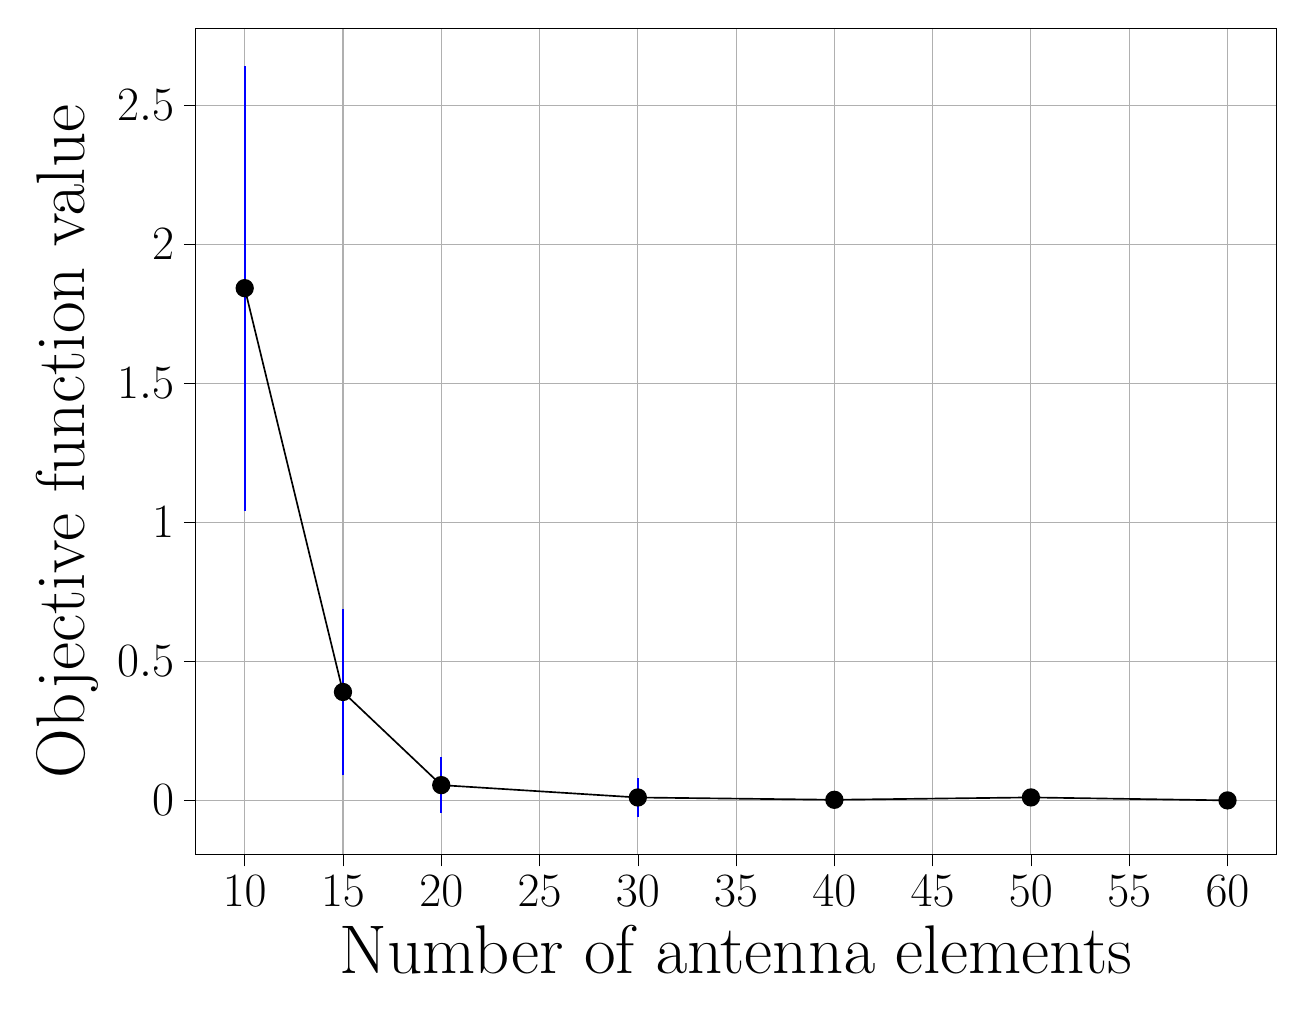
\begin{tikzpicture}

\begin{axis}[
width=6.028in,
height=4.754in,
xlabel style={font=\Huge},
ticklabel style={font=\LARGE},
ylabel style={font=\Huge},
tick align=outside,
tick pos=left,
x grid style={white!69.01960784313725!black},
xlabel={Number of antenna elements},
xmajorgrids,
xmin=7.5, xmax=62.5,
xtick style={color=black},
y grid style={white!69.01960784313725!black},
ylabel={Objective function value},
ymajorgrids,
ymin=-0.194615, ymax=2.777915,
ytick style={color=black}
]
\path [draw=blue, thick]
(axis cs:10,1.0428)
--(axis cs:10,2.6428);

\path [draw=blue, thick]
(axis cs:15,0.09)
--(axis cs:15,0.69);

\path [draw=blue, thick]
(axis cs:20,-0.045)
--(axis cs:20,0.155);

\path [draw=blue, thick]
(axis cs:30,-0.0595)
--(axis cs:30,0.0805);

\path [draw=blue, thick]
(axis cs:40,-0.0078)
--(axis cs:40,0.0122);

\path [draw=blue, thick]
(axis cs:50,0.0107)
--(axis cs:50,0.0107);

\path [draw=blue, thick]
(axis cs:60,0)
--(axis cs:60,0);

\addplot [semithick, black, mark=*, mark size=3, mark options={solid}]
table {%
10 1.8428
15 0.39
20 0.055
30 0.0105
40 0.0022
50 0.0107
60 0
};
\end{axis}

\end{tikzpicture}
    \end{adjustbox}
    \end{figure}  
\end{column}
\begin{column}{0.5\textwidth}
    \centering
    \textbf{Allocation of three frequencies}
    \begin{figure}[H]
    \centering
    \begin{adjustbox}{width=0.8\linewidth}
    % This file was created by matplotlib2tikz v0.7.5.
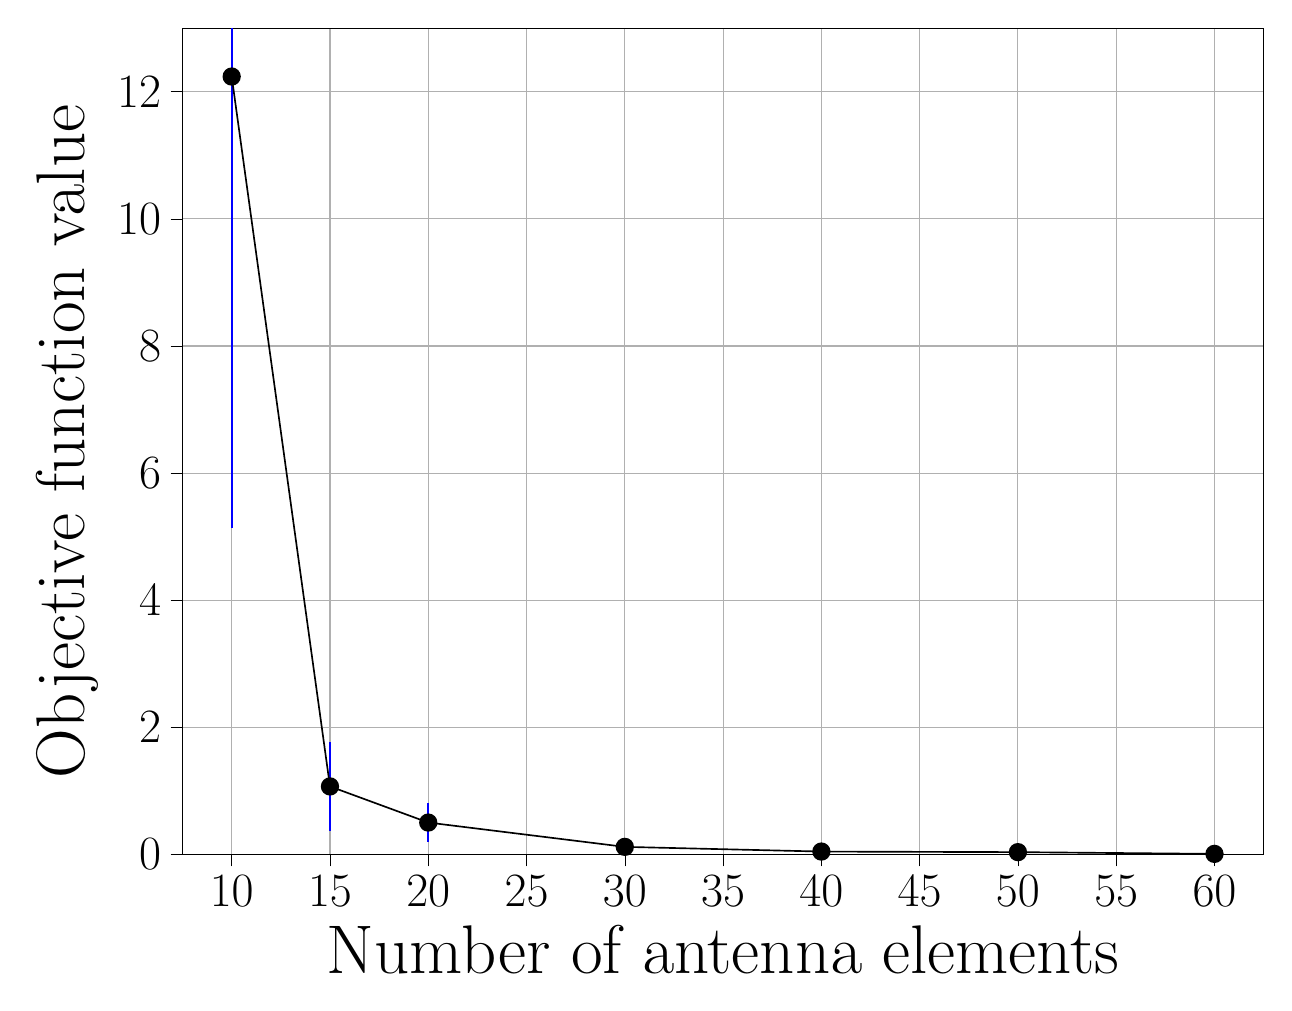
\begin{tikzpicture}

\begin{axis}[
width=6.028in,
height=4.754in,
xlabel style={font=\Huge},
ticklabel style={font=\LARGE},
ylabel style={font=\Huge},
tick align=outside,
tick pos=left,
x grid style={white!69.01960784313725!black},
xlabel={Number of antenna elements},
xmajorgrids,
xmin=7.5, xmax=62.5,
xtick style={color=black},
y grid style={white!69.01960784313725!black},
ylabel={Objective function value},
ymajorgrids,
ymin=0, ymax=13,
ytick style={color=black}
]
\path [draw=blue, thick]
(axis cs:10,5.14)
--(axis cs:10,14.34);

\path [draw=blue, thick]
(axis cs:15,0.371)
--(axis cs:15,1.771);

\path [draw=blue, thick]
(axis cs:20,0.2025)
--(axis cs:20,0.8025);

\path [draw=blue, thick]
(axis cs:30,0.1)
--(axis cs:30,0.14);

\path [draw=blue, thick]
(axis cs:40,0.036)
--(axis cs:40,0.056);

\path [draw=blue, thick]
(axis cs:50,0.037)
--(axis cs:50,0.037);

\path [draw=blue, thick]
(axis cs:60,0.0094)
--(axis cs:60,0.0094);

\addplot [semithick, black, mark=*, mark size=3, mark options={solid}]
table {%
10 12.24
15 1.071
20 0.5025
30 0.12
40 0.046
50 0.037
60 0.0094
};
\end{axis}

\end{tikzpicture}
    \end{adjustbox}
    \end{figure}  
\end{column}    
\end{columns}

\vspace{0.3cm}

\textbf{Experimental setup}:
\begin{itemize}
    \item 10 different antenna configurations are shown (averaged)
    \item Number of elements varied from $10$ to $60$
\end{itemize}

\end{frame}



\begin{frame}[t]{Results. Allocation of three frequencies}

\textbf{Note}:
\begin{itemize}
    \item $50$ elements, $d$ - distance between elements
    \item All units are normalised
\end{itemize}

\begin{columns}[b]
        \begin{column}{0.55\textwidth}
            \centering
            \begin{adjustbox}{width=1\columnwidth}
            % This file was created by matplotlib2tikz v0.7.4.
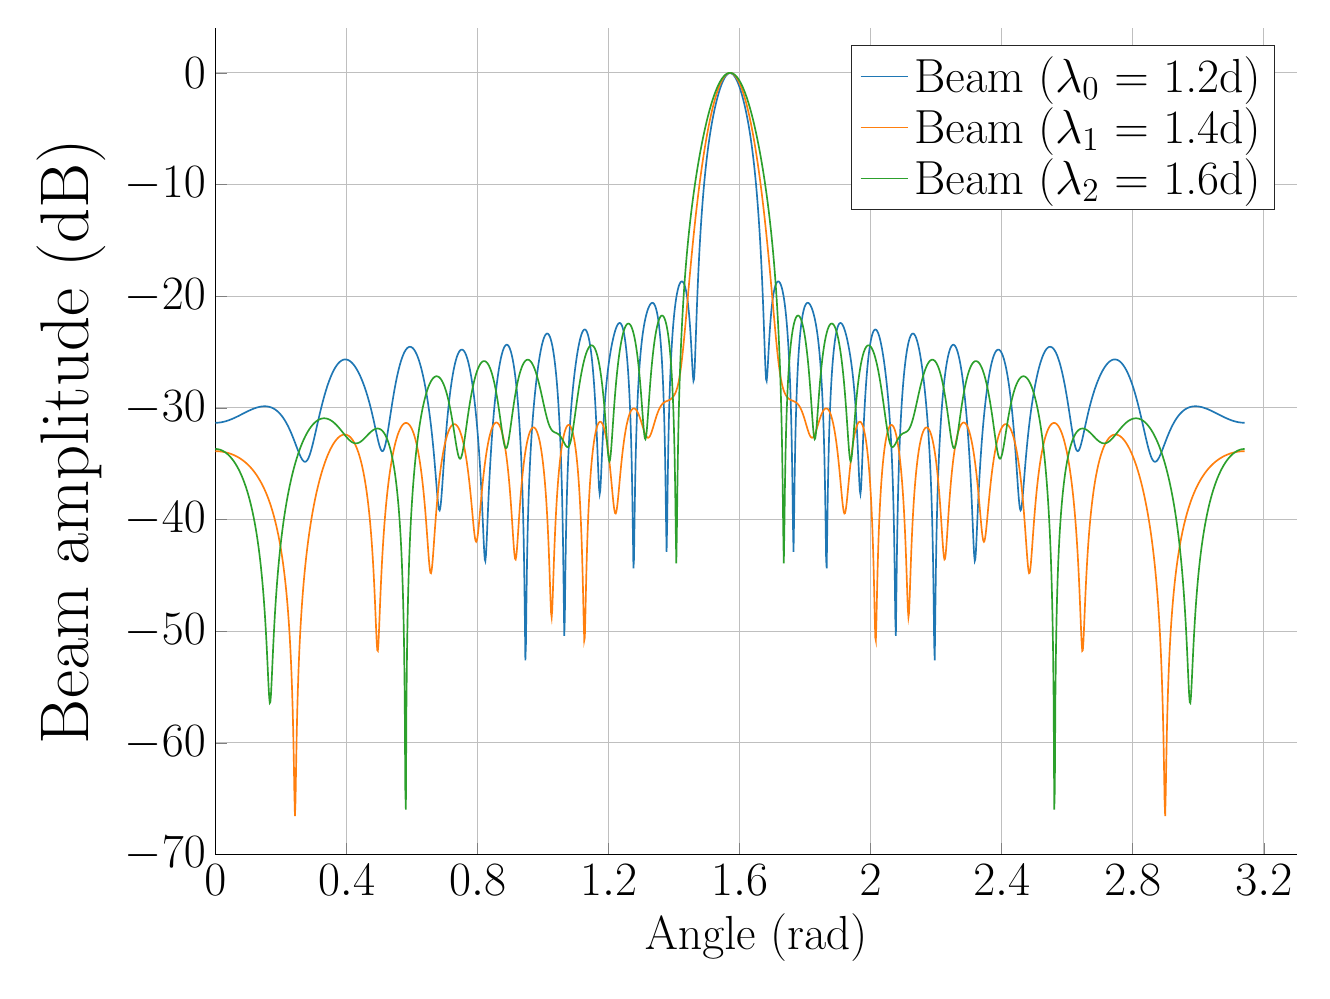
\begin{tikzpicture}

\definecolor{color0}{rgb}{0.12156862745098,0.466666666666667,0.705882352941177}
\definecolor{color1}{rgb}{1,0.498039215686275,0.0549019607843137}
\definecolor{color2}{rgb}{0.172549019607843,0.627450980392157,0.172549019607843}

\begin{axis}[
width=6.028in,
height=4.754in,
at={(1.011in,0.642in)},
% scale only axis,
xmin=0,
xmax=3.3,
xlabel={Angle (rad)},
xtick distance=0.4,
xmajorgrids,
ymin=-70,
ymax=4,
ylabel={Beam amplitude (dB)},
ymajorgrids,
axis background/.style={fill=white},
axis x line*=bottom,
axis y line*=left,
legend style={legend cell align=left,align=left,draw=white!15!black},
xlabel style={font=\LARGE},ylabel style={font=\Huge},legend style={font=\LARGE},ticklabel style={font=\LARGE}
% legend cell align={left},
% legend style={draw=white!80.0!black},
% tick align=outside,
% tick pos=left,
% x grid style={white!69.01960784313725!black},
% xlabel={Angle (rad)},
% xmajorgrids,
% xmin=-0.15707963267949, xmax=3.29867228626928,
% xtick style={color=black},
% y grid style={white!69.01960784313725!black},
% ylabel={Beam amplitude (dB)},
% ymajorgrids,
% ymin=-69.8951455095142, ymax=3.3309535933387,
% ytick style={color=black}
]
\addplot [semithick, color0]
table {%
0 -31.3353690916284
0.00174532925199433 -31.3349303409912
0.00349065850398866 -31.3336145861639
0.00523598775598299 -31.3314233176827
0.00698131700797732 -31.3283590174193
0.00872664625997165 -31.3244251550537
0.010471975511966 -31.3196261831631
0.0122173047639603 -31.3139675309344
0.0139626340159546 -31.3074555965462
0.015707963267949 -31.3000977382269
0.0174532925199433 -31.2919022640574
0.0191986217719376 -31.2828784205317
0.020943951023932 -31.2730363799406
0.0226892802759263 -31.2623872266254
0.0244346095279206 -31.2509429421619
0.0261799387799149 -31.2387163895205
0.0279252680319093 -31.2257212962946
0.0296705972839036 -31.2119722370357
0.0314159265358979 -31.1974846147804
0.0331612557878923 -31.1822746418403
0.0349065850398866 -31.1663593199314
0.0366519142918809 -31.1497564197096
0.0383972435438753 -31.1324844598092
0.0401425727958696 -31.11456268544
0.0418879020478639 -31.0960110466431
0.0436332312998582 -31.0768501762715
0.0453785605518526 -31.0571013677858
0.0471238898038469 -31.0367865529292
0.0488692190558412 -31.0159282793806
0.0506145483078356 -30.9945496884405
0.0523598775598299 -30.9726744928434
0.0541052068118242 -30.9503269547607
0.0558505360638185 -30.9275318640665
0.0575958653158129 -30.9043145169419
0.0593411945678072 -30.8807006948747
0.0610865238198015 -30.8567166441306
0.0628318530717959 -30.8323890557475
0.0645771823237902 -30.8077450461186
0.0663225115757845 -30.782812138212
0.0680678408277789 -30.7576182434931
0.0698131700797732 -30.7321916445776
0.0715584993317675 -30.7065609786848
0.0733038285837618 -30.6807552219161
0.0750491578357562 -30.6548036744038
0.0767944870877505 -30.6287359463696
0.0785398163397448 -30.6025819451197
0.0802851455917392 -30.5763718630079
0.0820304748437335 -30.5501361663969
0.0837758040957278 -30.5239055856297
0.0855211333477222 -30.497711106048
0.0872664625997165 -30.4715839600579
0.0890117918517108 -30.4455556202672
0.0907571211037051 -30.4196577937016
0.0925024503556995 -30.3939224171134
0.0942477796076938 -30.3683816533804
0.0959931088596881 -30.3430678890085
0.0977384381116825 -30.3180137327317
0.0994837673636768 -30.293252015216
0.101229096615671 -30.2688157898568
0.102974425867665 -30.2447383346766
0.10471975511966 -30.2210531552977
0.106465084371654 -30.1977939890114
0.108210413623648 -30.1749948098982
0.109955742875643 -30.1526898350193
0.111701072127637 -30.1309135316459
0.113446401379631 -30.1097006255246
0.115191730631626 -30.0890861101548
0.11693705988362 -30.0691052570666
0.118682389135614 -30.0497936270766
0.120427718387609 -30.0311870825062
0.122173047639603 -30.0133218003365
0.123918376891597 -29.9962342862804
0.125663706143592 -29.979961389742
0.127409035395586 -29.9645403196431
0.12915436464758 -29.9500086610826
0.130899693899575 -29.9364043927969
0.132645023151569 -29.9237659053938
0.134390352403563 -29.9121320203114
0.136135681655558 -29.9015420094737
0.137881010907552 -29.8920356155816
0.139626340159546 -29.8836530730077
0.141371669411541 -29.8764351292191
0.143116998663535 -29.8704230666819
0.144862327915529 -29.8656587251655
0.146607657167524 -29.8621845243713
0.148352986419518 -29.8600434867988
0.150098315671512 -29.859279260739
0.151843644923507 -29.8599361432881
0.153588974175501 -29.8620591032416
0.155334303427495 -29.8656938037221
0.15707963267949 -29.8708866243677
0.158824961931484 -29.8776846828795
0.160570291183478 -29.8861358557077
0.162315620435473 -29.8962887976091
0.164060949687467 -29.9081929597776
0.165806278939461 -29.9218986062154
0.167551608191456 -29.9374568279275
0.16929693744345 -29.9549195545059
0.171042266695444 -29.9743395625638
0.172787595947439 -29.9957704804311
0.174532925199433 -30.0192667884
0.176278254451427 -30.0448838137299
0.178023583703422 -30.0726777194923
0.179768912955416 -30.10270548618
0.18151424220741 -30.1350248848666
0.183259571459405 -30.1696944404952
0.185004900711399 -30.2067733836713
0.186750229963393 -30.246321589079
0.188495559215388 -30.2883994983557
0.190240888467382 -30.3330680249278
0.191986217719376 -30.3803884379208
0.193731546971371 -30.4304222218442
0.195476876223365 -30.4832309081951
0.197222205475359 -30.5388758746083
0.198967534727354 -30.5974181064457
0.200712863979348 -30.6589179150047
0.202458193231342 -30.7234346056161
0.204203522483337 -30.7910260879141
0.205948851735331 -30.8617484194072
0.207694180987325 -30.9356552722071
0.20943951023932 -31.0127973112637
0.211184839491314 -31.0932214708627
0.212930168743308 -31.1769701142396
0.214675497995303 -31.2640800591696
0.216420827247297 -31.3545814501074
0.218166156499291 -31.4484964550592
0.219911485751286 -31.5458377627442
0.22165681500328 -31.6466068529299
0.223402144255274 -31.7507920101146
0.225147473507269 -31.8583660481313
0.226892802759263 -31.969283710986
0.228638132011257 -32.0834787135738
0.230383461263252 -32.20086038525
0.232128790515246 -32.3213098800858
0.23387411976724 -32.444675920778
0.235619449019234 -32.5707700494481
0.237364778271229 -32.6993613692446
0.239110107523223 -32.8301707771241
0.240855436775217 -32.9628647122273
0.242600766027212 -33.0970484779419
0.244346095279206 -33.2322592410982
0.246091424531201 -33.3679588710803
0.247836753783195 -33.5035268566222
0.249582083035189 -33.6382536295555
0.251327412287183 -33.7713347320237
0.253072741539178 -33.901866383006
0.254818070791172 -34.0288431239319
0.256563400043166 -34.1511583388361
0.258308729295161 -34.2676085326357
0.260054058547155 -34.3769022858695
0.261799387799149 -34.4776747541311
0.263544717051144 -34.5685084120429
0.265290046303138 -34.6479604258613
0.267035375555132 -34.7145965603464
0.268780704807127 -34.7670308941367
0.270526034059121 -34.8039698782131
0.272271363311115 -34.824258509954
0.27401669256311 -34.8269257312941
0.275762021815104 -34.8112257329483
0.277507351067098 -34.7766717833899
0.279252680319093 -34.7230595786665
0.280998009571087 -34.6504779242502
0.282743338823081 -34.5593057174017
0.284488668075076 -34.4501955231892
0.28623399732707 -34.3240453139565
0.287979326579064 -34.1819609672694
0.289724655831059 -34.025212747337
0.291469985083053 -33.8551891747717
0.293215314335047 -33.6733514541859
0.294960643587042 -33.4811910816987
0.296705972839036 -33.2801925309514
0.29845130209103 -33.0718021508669
0.300196631343025 -32.8574037080068
0.301941960595019 -32.6383004385682
0.303687289847013 -32.4157030683144
0.305432619099008 -32.1907230103182
0.307177948351002 -31.964369837772
0.308923277602996 -31.7375521202004
0.310668606854991 -31.5110807731044
0.312413936106985 -31.2856741740328
0.314159265358979 -31.0619644193371
0.315904594610974 -30.8405042190162
0.317649923862968 -30.6217740417779
0.319395253114962 -30.4061892230464
0.321140582366957 -30.1941068329101
0.322885911618951 -29.9858321689751
0.324631240870945 -29.7816247920459
0.32637657012294 -29.5817040625621
0.328121899374934 -29.3862541648859
0.329867228626928 -29.1954286270444
0.331612557878923 -29.009354357273
0.333357887130917 -28.8281352272711
0.335103216382911 -28.6518552368697
0.336848545634906 -28.4805812968327
0.3385938748869 -28.314365666636
0.340339204138894 -28.1532480829094
0.342084533390889 -27.9972576122438
0.343829862642883 -27.8464142596451
0.345575191894877 -27.7007303612402
0.347320521146872 -27.5602117871294
0.349065850398866 -27.4248589776454
0.35081117965086 -27.294667833727
0.352556508902855 -27.1696304797925
0.354301838154849 -27.0497359153436
0.356047167406843 -26.9349705695676
0.357792496658838 -26.8253187714834
0.359537825910832 -26.7207631465957
0.361283155162826 -26.6212849496643
0.363028484414821 -26.5268643419752
0.364773813666815 -26.4374806204403
0.366519142918809 -26.3531124049362
0.368264472170804 -26.2737377894757
0.370009801422798 -26.1993344621274
0.371755130674792 -26.129879797987
0.373500459926787 -26.0653509290093
0.375245789178781 -26.0057247940532
0.376991118430775 -25.9509781721459
0.37873644768277 -25.9010877016465
0.380481776934764 -25.8560298877474
0.382227106186758 -25.8157811005306
0.383972435438752 -25.7803175656425
0.385717764690747 -25.7496153495112
0.387463093942741 -25.7236503409388
0.389208423194735 -25.7023982308342
0.39095375244673 -25.6858344918113
0.392699081698724 -25.6739343593603
0.394444410950719 -25.6666728162982
0.396189740202713 -25.6640245822353
0.397935069454707 -25.6659641098174
0.399680398706702 -25.6724655895511
0.401425727958696 -25.683502965082
0.40317105721069 -25.6990499608394
0.404916386462685 -25.7190801240311
0.406661715714679 -25.7435668830163
0.408407044966673 -25.7724836241397
0.410152374218667 -25.8058037891271
0.411897703470662 -25.8435009951711
0.413643032722656 -25.8855491797949
0.41538836197465 -25.9319227725496
0.417133691226645 -25.9825968954936
0.418879020478639 -26.0375475942522
0.420624349730633 -26.0967521012442
0.422369678982628 -26.1601891323788
0.424115008234622 -26.2278392181437
0.425860337486616 -26.2996850695413
0.427605666738611 -26.3757119787359
0.429350995990605 -26.4559082535696
0.431096325242599 -26.5402656842385
0.432841654494594 -26.6287800394055
0.434586983746588 -26.7214515878172
0.436332312998582 -26.8182856400824
0.438077642250577 -26.9192931036308
0.439822971502571 -27.024491041938
0.441568300754565 -27.1339032269046
0.44331363000656 -27.247560670655
0.445058959258554 -27.3655021200463
0.446804288510548 -27.4877744936103
0.448549617762543 -27.6144332365253
0.450294947014537 -27.7455425642939
0.452040276266531 -27.8811755599461
0.453785605518526 -28.02141408259
0.45553093477052 -28.166348436655
0.457276264022514 -28.3160767409259
0.459021593274509 -28.4707039239696
0.460766922526503 -28.6303402573162
0.462512251778497 -28.7950993191099
0.464257581030492 -28.9650952582178
0.466002910282486 -29.1404392011206
0.46774823953448 -29.3212346104549
0.469493568786475 -29.5075713640662
0.471238898038469 -29.699518276126
0.472984227290463 -29.8971137271835
0.474729556542458 -30.1003540086221
0.476474885794452 -30.3091789211387
0.478220215046446 -30.5234541016274
0.479965544298441 -30.7429494974257
0.481710873550435 -30.9673133772844
0.483456202802429 -31.196041290416
0.485201532054424 -31.4284394983404
0.486946861306418 -31.6635826671989
0.488692190558412 -31.900266101167
0.490437519810407 -32.136953623752
0.492182849062401 -32.3717234901984
0.493928178314395 -32.6022165468276
0.49567350756639 -32.825593281445
0.497418836818384 -33.0385093118579
0.499164166070378 -33.237121819419
0.500909495322373 -33.4171415913294
0.502654824574367 -33.5739453171116
0.504400153826361 -33.7027588726248
0.506145483078356 -33.7989130360448
0.50789081233035 -33.8581582172646
0.509636141582344 -33.8770066240856
0.511381470834339 -33.8530540822122
0.513126800086333 -33.7852264647555
0.514872129338327 -33.6739029384921
0.516617458590322 -33.5208904383585
0.518362787842316 -33.3292546906543
0.52010811709431 -33.1030421683158
0.521853446346305 -32.8469449603959
0.523598775598299 -32.5659625916272
0.525344104850293 -32.2651038190422
0.527089434102288 -31.9491538379009
0.528834763354282 -31.6225148275548
0.530580092606276 -31.2891146518858
0.53232542185827 -30.9523711419174
0.534070751110265 -30.6151969670223
0.535816080362259 -30.2800309887752
0.537561409614253 -29.9488845437591
0.539306738866248 -29.623394114166
0.541052068118242 -29.304874619071
0.542797397370236 -28.994369792715
0.544542726622231 -28.6926977546839
0.546288055874225 -28.4004909904064
0.548033385126219 -28.1182306629203
0.549778714378214 -27.8462755826444
0.551524043630208 -27.5848863668346
0.553269372882203 -27.3342453973075
0.555014702134197 -27.0944731854539
0.556760031386191 -26.8656417121808
0.558505360638185 -26.6477852493207
0.56025068989018 -26.4409091017349
0.561996019142174 -26.2449966434262
0.563741348394169 -26.0600149604631
0.565486677646163 -25.8859193601269
0.567232006898157 -25.7226569597605
0.568977336150151 -25.5701695300418
0.570722665402146 -25.4283957350916
0.57246799465414 -25.2972728851682
0.574213323906134 -25.1767382958267
0.575958653158129 -25.0667303296378
0.577703982410123 -24.9671891820785
0.579449311662117 -24.8780574615464
0.581194640914112 -24.7992806040251
0.582939970166106 -24.7308071553886
0.5846852994181 -24.6725889483168
0.586430628670095 -24.6245811960083
0.588175957922089 -24.586742521157
0.589921287174083 -24.5590349357617
0.591666616426078 -24.5414237851719
0.593411945678072 -24.5338776682216
0.595157274930066 -24.5363683442475
0.596902604182061 -24.5488706372402
0.598647933434055 -24.5713623471809
0.600393262686049 -24.6038241788735
0.602138591938044 -24.6462396991343
0.603883921190038 -24.6985953341438
0.605629250442032 -24.7608804200297
0.607374579694027 -24.8330873213399
0.609119908946021 -24.9152116340152
0.610865238198015 -25.0072524917144
0.61261056745001 -25.1092129969516
0.614355896702004 -25.2211008013872
0.616101225953998 -25.3429288628159
0.617846555205993 -25.4747164098342
0.619591884457987 -25.6164901488281
0.621337213709981 -25.7682857517049
0.623082542961976 -25.9301496666252
0.62482787221397 -26.1021412977257
0.626573201465964 -26.2843356033113
0.628318530717959 -26.4768261650209
0.630063859969953 -26.6797287827471
0.631809189221947 -26.8931856513082
0.633554518473942 -27.1173701745363
0.635299847725936 -27.3524924699486
0.63704517697793 -27.5988056116719
0.638790506229925 -27.8566126494998
0.640535835481919 -28.1262744260302
0.642281164733913 -28.4082181888609
0.644026493985908 -28.7029469562722
0.645771823237902 -29.0110495355941
0.647517152489896 -29.3332110019816
0.649262481741891 -29.6702233033433
0.651007810993885 -30.0229954349432
0.652753140245879 -30.392562276963
0.654498469497874 -30.7800906326029
0.656243798749868 -31.1868801175776
0.657989128001862 -31.6143551305312
0.659734457253857 -32.0640418485128
0.661479786505851 -32.537520512399
0.663225115757845 -33.0363373561558
0.66497044500984 -33.561851107563
0.666715774261834 -34.1149742107297
0.668461103513828 -34.6957465530751
0.670206432765823 -35.3026479801808
0.671951762017817 -35.9315183239298
0.673697091269811 -36.5739287280678
0.675442420521806 -37.2148953366333
0.6771877497738 -37.8300887870931
0.678933079025794 -38.383412690108
0.680678408277788 -38.8271381497146
0.682423737529783 -39.1079473396294
0.684169066781777 -39.1807329690396
0.685914396033772 -39.0255911658334
0.687659725285766 -38.6568571084942
0.68940505453776 -38.1167679204347
0.691150383789755 -37.4590403303283
0.692895713041749 -36.7338420018252
0.694641042293743 -35.9802780407105
0.696386371545738 -35.2253949911615
0.698131700797732 -34.4863264574075
0.699877030049726 -33.773109013441
0.701622359301721 -33.0910869850131
0.703367688553715 -32.442659022201
0.705113017805709 -31.8284482524343
0.706858347057703 -31.2480517582509
0.708603676309698 -30.7005074537447
0.710349005561692 -30.1845790340183
0.712094334813687 -29.6989264981063
0.713839664065681 -29.2422056755627
0.715584993317675 -28.813124119674
0.717330322569669 -28.4104704258898
0.719075651821664 -28.033127554064
0.720820981073658 -27.68007669455
0.722566310325653 -27.3503957095708
0.724311639577647 -27.0432546235909
0.726056968829641 -26.7579096685856
0.727802298081635 -26.4936967883466
0.72954762733363 -26.250025132144
0.731292956585624 -26.0263708364676
0.733038285837618 -25.8222712510526
0.734783615089613 -25.6373196787229
0.736528944341607 -25.4711606469789
0.738274273593601 -25.3234856996349
0.740019602845596 -25.1940296808715
0.74176493209759 -25.0825674766668
0.743510261349584 -24.9889111763336
0.745255590601579 -24.9129076178159
0.747000919853573 -24.8544362831571
0.748746249105568 -24.8134075143822
0.750491578357562 -24.789761024471
0.752236907609556 -24.7834646829204
0.75398223686155 -24.7945135604636
0.755727566113545 -24.8229292228957
0.757472895365539 -24.8687592696757
0.759218224617533 -24.9320771192254
0.760963553869528 -25.0129820498091
0.762708883121522 -25.1115995128298
0.764454212373516 -25.2280817446468
0.766199541625511 -25.3626087140669
0.767944870877505 -25.5153894559329
0.769690200129499 -25.6866638574662
0.771435529381494 -25.876704983931
0.773180858633488 -26.0858220548087
0.774926187885482 -26.3143642121868
0.776671517137477 -26.5627252609437
0.778416846389471 -26.8313496073675
0.780162175641465 -27.1207396811936
0.78190750489346 -27.4314651982491
0.783652834145454 -27.7641747098364
0.785398163397448 -28.1196099938751
0.787143492649443 -28.4986239747297
0.788888821901437 -28.9022030160038
0.790634151153431 -29.3314946133593
0.792379480405426 -29.7878417170623
0.79412480965742 -30.2728251185333
0.795870138909414 -30.7883154972978
0.797615468161409 -31.3365367447862
0.799360797413403 -31.9201418436238
0.801106126665397 -32.542301425348
0.802851455917392 -33.20680217514
0.804596785169386 -33.9181453951367
0.80634211442138 -34.6816207141054
0.808087443673375 -35.5032961183927
0.809832772925369 -36.3897909665094
0.811578102177363 -37.3475342988414
0.813323431429358 -38.3808511114939
0.815068760681352 -39.4874617244447
0.816814089933346 -40.6485739234839
0.818559419185341 -41.8091663799638
0.820304748437335 -42.8472635023244
0.822050077689329 -43.5558569979732
0.823795406941324 -43.7106629861787
0.825540736193318 -43.2424176711756
0.827286065445312 -42.3064558710383
0.829031394697307 -41.1372466805738
0.830776723949301 -39.9078996216788
0.832522053201295 -38.7087866182681
0.83426738245329 -37.5769238277444
0.836012711705284 -36.522763584659
0.837758040957278 -35.5452534358431
0.839503370209273 -34.6390279997984
0.841248699461267 -33.7975868947553
0.842994028713261 -33.01460653107
0.844739357965256 -32.284418338124
0.84648468721725 -31.6021262452326
0.848230016469244 -30.9635762756801
0.849975345721239 -30.3652729904121
0.851720674973233 -29.8042840020583
0.853466004225227 -29.2781495269831
0.855211333477221 -28.7848030199386
0.856956662729216 -28.3225041297173
0.85870199198121 -27.8897832237155
0.860447321233205 -27.4853960259327
0.862192650485199 -27.1082867827098
0.863937979737193 -26.7575584794986
0.865683308989187 -26.4324488252191
0.867428638241182 -26.132310928608
0.869173967493176 -25.8565977840944
0.870919296745171 -25.6048498528839
0.872664625997165 -25.3766851664754
0.874409955249159 -25.171791496845
0.876155284501153 -24.9899202333738
0.877900613753148 -24.8308816848891
0.879645943005142 -24.6945415892902
0.881391272257136 -24.5808186661242
0.883136601509131 -24.4896830917366
0.884881930761125 -24.421155814452
0.88662726001312 -24.375308660567
0.888372589265114 -24.352265212496
0.890117918517108 -24.3522024697923
0.891863247769102 -24.3753533335994
0.893608577021097 -24.4220099870426
0.895353906273091 -24.4925282800705
0.897099235525086 -24.5873332696055
0.89884456477708 -24.7069261174321
0.900589894029074 -24.8518926128273
0.902335223281068 -25.022913669576
0.904080552533063 -25.2207782546745
0.905825881785057 -25.4463993484431
0.907571211037051 -25.7008337267893
0.909316540289046 -25.9853066160061
0.91106186954104 -26.3012426281383
0.912807198793034 -26.6503048844463
0.914552528045029 -27.0344449424371
0.916297857297023 -27.4559671612719
0.918043186549017 -27.9176126336386
0.919788515801012 -28.4226700415152
0.921533845053006 -28.9751241917741
0.923279174305 -29.5798582899325
0.925024503556995 -30.24293449945
0.926769832808989 -30.9719913233358
0.928515162060983 -31.7768201581316
0.930260491312978 -32.6702254152439
0.932005820564972 -33.6693499645049
0.933751149816966 -34.7977967520352
0.935496479068961 -36.0891799676156
0.937241808320955 -37.5933871497784
0.938987137572949 -39.3882881400255
0.940732466824944 -41.6028681856566
0.942477796076938 -44.4624473119736
0.944223125328932 -48.3233133020577
0.945968454580927 -52.6095883748369
0.947713783832921 -51.1597068071725
0.949459113084915 -46.8228780541194
0.95120444233691 -43.5226160385931
0.952949771588904 -41.0663000695915
0.954695100840898 -39.1423980062047
0.956440430092893 -37.5701304344139
0.958185759344887 -36.2436950056659
0.959931088596881 -35.0972916198348
0.961676417848876 -34.0876445693456
0.96342174710087 -33.1849790441985
0.965167076352864 -32.3680767353269
0.966912405604859 -31.6214059676079
0.968657734856853 -30.9333682425921
0.970403064108847 -30.2951772188482
0.972148393360842 -29.7001125244506
0.973893722612836 -29.1430048235165
0.97563905186483 -28.6198688791268
0.977384381116825 -28.1276346556274
0.979129710368819 -27.6639455638671
0.980875039620813 -27.227004194448
0.982620368872808 -26.8154526797538
0.984365698124802 -26.4282790205354
0.986111027376796 -26.0647433532065
0.987856356628791 -25.7243198302567
0.989601685880785 -25.4066509027846
0.991347015132779 -25.11151155169
0.993092344384774 -24.8387815470242
0.994837673636768 -24.5884242054362
0.996583002888762 -24.3604704135144
0.998328332140757 -24.155006920418
1.00007366139275 -23.9721680950517
1.00181899064475 -23.8121305025873
1.00356431989674 -23.6751097898659
1.00530964914873 -23.5613594842337
1.00705497840073 -23.4711714096412
1.00880030765272 -23.4048775106687
1.01054563690472 -23.3628529525949
1.01229096615671 -23.3455204366831
1.01403629540871 -23.353355737657
1.0157816246607 -23.3868945382553
1.01752695391269 -23.4467407076806
1.01927228316469 -23.5335762513519
1.02101761241668 -23.6481732544647
1.02276294166868 -23.7914082590905
1.02450827092067 -23.9642796642003
1.02625360017267 -24.1679289344508
1.02799892942466 -24.4036666672467
1.02974425867665 -24.6730049283301
1.03148958792865 -24.9776977682257
1.03323491718064 -25.3197925424108
1.03498024643264 -25.7016956808163
1.03672557568463 -26.1262580507772
1.03847090493663 -26.5968872957009
1.04021623418862 -27.1176979452696
1.04196156344061 -27.6937154208213
1.04370689269261 -28.3311585910365
1.0454522219446 -29.0378395910151
1.0471975511966 -29.82374353678
1.04894288044859 -30.7018929569877
1.05068820970059 -31.6896792548651
1.05243353895258 -32.8109924254951
1.05417886820458 -34.0997808895563
1.05592419745657 -35.6063114376925
1.05766952670856 -37.4088050050634
1.05941485596056 -39.636101840663
1.06116018521255 -42.5099817238104
1.06290551446455 -46.358343141092
1.06465084371654 -50.4296791176593
1.06639617296854 -48.8626416415239
1.06814150222053 -44.6920125862632
1.06988683147252 -41.4947128328877
1.07163216072452 -39.109508941672
1.07337748997651 -37.2451025789099
1.07512281922851 -35.7282128740917
1.0768681484805 -34.4560100300659
1.0786134777325 -33.3638854477944
1.08035880698449 -32.4089532505681
1.08210413623648 -31.56142932761
1.08384946548848 -30.7998778026909
1.08559479474047 -30.1084451494685
1.08734012399247 -29.4751709196703
1.08908545324446 -28.8909101867119
1.09083078249646 -28.3486181684072
1.09257611174845 -27.8428569850161
1.09432144100044 -27.36944298827
1.09606677025244 -26.9251857440901
1.09781209950443 -26.5076886771217
1.09955742875643 -26.115192683951
1.10130275800842 -25.7464509017544
1.10304808726042 -25.4006270473304
1.10479341651241 -25.0772123382759
1.10653874576441 -24.7759575896863
1.1082840750164 -24.4968180324419
1.11002940426839 -24.2399089704119
1.11177473352039 -24.0054707429442
1.11352006277238 -23.7938416862426
1.11526539202438 -23.6054379536226
1.11701072127637 -23.4407391946957
1.11875605052837 -23.3002792249174
1.12050137978036 -23.1846409471126
1.12224670903235 -23.0944549175657
1.12399203828435 -23.0304010806999
1.12573736753634 -22.9932133274319
1.12748269678834 -22.983686662835
1.12922802604033 -23.0026868997079
1.13097335529233 -23.0511629284274
1.13271868454432 -23.1301617538681
1.13446401379631 -23.2408466425043
1.13620934304831 -23.3845188938059
1.1379546723003 -23.5626439477337
1.1397000015523 -23.7768827733464
1.14144533080429 -24.0291297604918
1.14319066005629 -24.3215586614852
1.14493598930828 -24.65667849476
1.14668131856027 -25.0374016896543
1.14842664781227 -25.4671270118763
1.15017197706426 -25.9498396921497
1.15191730631626 -26.4902300494473
1.15366263556825 -27.093828285776
1.15540796482025 -27.7671436465008
1.15715329407224 -28.5177729246595
1.15889862332423 -29.3543878363267
1.16064395257623 -30.2863790730069
1.16238928182822 -31.3226220818297
1.16413461108022 -32.4680952918197
1.16587994033221 -33.7154480426706
1.16762526958421 -35.025634864157
1.1693705988362 -36.2901270022904
1.1711159280882 -37.2861069499612
1.17286125734019 -37.7126348212326
1.17460658659218 -37.4124183816747
1.17635191584418 -36.5433880606379
1.17809724509617 -35.4054032921759
1.17984257434817 -34.2194013247186
1.18158790360016 -33.0921903238279
1.18333323285216 -32.0613696650734
1.18507856210415 -31.1329952222929
1.18682389135614 -30.300854025686
1.18856922060814 -29.5548560209227
1.19031454986013 -28.8844053554751
1.19205987911213 -28.2796399144328
1.19380520836412 -27.731801689569
1.19555053761612 -27.2332697815209
1.19729586686811 -26.7774764250204
1.1990411961201 -26.3587950560016
1.2007865253721 -25.9724339425099
1.20253185462409 -25.6143455338258
1.20427718387609 -25.2811520933357
1.20602251312808 -24.9700845931581
1.20776784238008 -24.678930920059
1.20951317163207 -24.405989707175
1.21125850088406 -24.1500268942492
1.21300383013606 -23.9102330957691
1.21474915938805 -23.6861808308031
1.21649448864005 -23.4777815197764
1.21823981789204 -23.2852428074881
1.21998514714404 -23.1090271942451
1.22173047639603 -22.9498131509359
1.22347580564803 -22.8084598924221
1.22522113490002 -22.6859768400079
1.22696646415201 -22.5834985791863
1.22871179340401 -22.502265871871
1.230457122656 -22.4436130613201
1.232202451908 -22.4089620480034
1.23394778115999 -22.3998229379606
1.23569311041199 -22.4178014843441
1.23743843966398 -22.4646135656165
1.23918376891597 -22.5421071788909
1.24092909816797 -22.6522927895508
1.24267442741996 -22.7973833977235
1.24441975667196 -22.9798464101642
1.24616508592395 -23.2024704299797
1.24791041517595 -23.4684515403259
1.24965574442794 -23.7815057977783
1.25140107367993 -24.1460178572506
1.25314640293193 -24.567240581847
1.25489173218392 -25.0515682852006
1.25663706143592 -25.6069189302204
1.25838239068791 -26.2432818660774
1.26012771993991 -26.9735245325424
1.2618730491919 -27.8146177429599
1.26361837844389 -28.7895625471332
1.26536370769589 -29.9305401504112
1.26710903694788 -31.284278765087
1.26885436619988 -32.9215455815768
1.27059969545187 -34.954011399104
1.27234502470387 -37.5587752995646
1.27409035395586 -40.9403194554309
1.27583568320786 -44.3699006611061
1.27758101245985 -43.5465179652775
1.27932634171184 -39.8675044166612
1.28107167096384 -36.7368880101102
1.28281700021583 -34.3334324385207
1.28456232946783 -32.4395665860215
1.28630765871982 -30.8994043814074
1.28805298797182 -29.6152020196996
1.28979831722381 -28.5240932362984
1.2915436464758 -27.5838104232392
1.2932889757278 -26.7646990458438
1.29503430497979 -26.0451602145308
1.29677963423179 -25.4089455707565
1.29852496348378 -24.8434866413494
1.30027029273578 -24.3388258403702
1.30201562198777 -23.8869115789373
1.30376095123976 -23.4811219561867
1.30550628049176 -23.1159367554017
1.30725160974375 -22.7867084739799
1.30899693899575 -22.4895010888246
1.31074226824774 -22.2209759860083
1.31248759749974 -21.9783110620804
1.31423292675173 -21.7591431530675
1.31597825600372 -21.5615266534034
1.31772358525572 -21.3839030344259
1.31946891450771 -21.2250773116202
1.32121424375971 -21.0841985510864
1.3229595730117 -20.9607423685412
1.3247049022637 -20.8544941195261
1.32645023151569 -20.7655321310123
1.32819556076768 -20.6942108846571
1.32994089001968 -20.6411445247311
1.33168621927167 -20.6071914249491
1.33343154852367 -20.5934408120607
1.33517687777566 -20.6012026254721
1.33692220702766 -20.6320019186172
1.33866753627965 -20.6875792171109
1.34041286553165 -20.7698983878022
1.34215819478364 -20.88116379746
1.34390352403563 -21.0238489173687
1.34564885328763 -21.2007391469859
1.34739418253962 -21.4149926059847
1.34913951179162 -21.6702241587868
1.35088484104361 -21.9706202726037
1.35263017029561 -22.3210959360085
1.3543754995476 -22.7275105742849
1.35612082879959 -23.1969690816323
1.35786615805159 -23.7382492627103
1.35961148730358 -24.3624228343508
1.36135681655558 -25.0837827881577
1.36310214580757 -25.921273718599
1.36484747505957 -26.9007822317283
1.36659280431156 -28.0589655971433
1.36833813356355 -29.4499625278231
1.37008346281555 -31.1577067532052
1.37182879206754 -33.3188551033977
1.37357412131954 -36.1572816432281
1.37531945057153 -39.8977856260141
1.37706477982353 -42.9011402569199
1.37881010907552 -40.3433698739741
1.38055543832751 -36.4318981583301
1.38230076757951 -33.4094869921424
1.3840460968315 -31.0994319461192
1.3857914260835 -29.2654848103139
1.38753675533549 -27.7618490958739
1.38928208458749 -26.4994241934862
1.39102741383948 -25.4211096180347
1.39277274309148 -24.4884745353911
1.39451807234347 -23.6745292409435
1.39626340159546 -22.9596283835772
1.39800873084746 -22.3290365413797
1.39975406009945 -21.7714180911909
1.40149938935145 -21.2778649313813
1.40324471860344 -20.8412504709651
1.40499004785544 -20.45578906979
1.40673537710743 -20.1167292841898
1.40848070635942 -19.8201369746928
1.41022603561142 -19.5627405028119
1.41197136486341 -19.3418199865723
1.41371669411541 -19.155128623122
1.4154620233674 -19.0008379280773
1.4172073526194 -18.8775012472604
1.41895268187139 -18.7840315771896
1.42069801112338 -18.7196908979953
1.42244334037538 -18.6840890737617
1.42418866962737 -18.6771910396436
1.42593399887937 -18.6993315589478
1.42767932813136 -18.7512373546023
1.42942465738336 -18.8340569339115
1.43116998663535 -18.9493989469756
1.43291531588734 -19.099380430993
1.43466064513934 -19.2866867240049
1.43640597439133 -19.5146450017802
1.43815130364333 -19.7873128838612
1.43989663289532 -20.1095814333939
1.44164196214732 -20.4872860409094
1.44338729139931 -20.9273043870665
1.44513262065131 -21.4375870512428
1.4468779499033 -22.0269881603733
1.44862327915529 -22.704581962018
1.45036860840729 -23.4777314249665
1.45211393765928 -24.3472303581678
1.45385926691128 -25.2959211594253
1.45560459616327 -26.2645588171227
1.45734992541527 -27.1117527700321
1.45909525466726 -27.5893413968973
1.46084058391925 -27.4378713724065
1.46258591317125 -26.6136372697964
1.46433124242324 -25.3369254156019
1.46607657167524 -23.8777925140507
1.46782190092723 -22.4093130491613
1.46956723017923 -21.0103756652106
1.47131255943122 -19.7074841328409
1.47305788868321 -18.5037740036587
1.47480321793521 -17.393360640593
1.4765485471872 -16.3675973489987
1.4782938764392 -15.4176115854772
1.48003920569119 -14.5352358343149
1.48178453494319 -13.713269806649
1.48352986419518 -12.9454767541461
1.48527519344717 -12.2264848951165
1.48702052269917 -11.5516651055601
1.48876585195116 -10.9170130230717
1.49051118120316 -10.3190452939048
1.49225651045515 -9.75471199176625
1.49400183970715 -9.22132421867256
1.49574716895914 -8.71649490756996
1.49749249821114 -8.23809070465665
1.49923782746313 -7.78419299352014
1.50098315671512 -7.35306640502256
1.50272848596712 -6.94313344101955
1.50447381521911 -6.5529540908547
1.50621914447111 -6.18120952775257
1.5079644737231 -5.82668913926249
1.5097098029751 -5.48828027730947
1.51145513222709 -5.16496021570272
1.51320046147908 -4.85578988235392
1.51494579073108 -4.55990899548146
1.51669111998307 -4.27653228239407
1.51843644923507 -4.00494649991432
1.52018177848706 -3.74450801022558
1.52192710773906 -3.49464069728978
1.52367243699105 -3.25483403872416
1.52541776624304 -3.02464117726343
1.52716309549504 -2.80367686521892
1.52890842474703 -2.59161518475321
1.53065375399903 -2.38818697596924
1.53239908325102 -2.19317693313282
1.53414441250302 -2.00642035599317
1.53588974175501 -1.82779956726555
1.537635071007 -1.65724002809674
1.539380400259 -1.49470620010384
1.54112572951099 -1.34019721495838
1.54287105876299 -1.19374242034917
1.54461638801498 -1.05539687463817
1.54636171726698 -0.925236862022422
1.54810704651897 -0.803355496117163
1.54985237577096 -0.689858473309748
1.55159770502296 -0.584860028789748
1.55334303427495 -0.488479138626337
1.55508836352695 -0.4008360013745
1.55683369277894 -0.32204882307963
1.55857902203094 -0.252230920728372
1.56032435128293 -0.191488151538091
1.56206968053493 -0.139916669229004
1.56381500978692 -0.0976010037037125
1.56556033903891 -0.0646124573783302
1.56730566829091 -0.0410078096961154
1.5690509975429 -0.0268283209655331
1.5707963267949 -0.0220990274093593
1.57254165604689 -0.0268283209655331
1.57428698529889 -0.0410078096961174
1.57603231455088 -0.064612457378336
1.57777764380287 -0.0976010037037193
1.57952297305487 -0.139916669229007
1.58126830230686 -0.191488151538101
1.58301363155886 -0.252230920728385
1.58475896081085 -0.322048823079634
1.58650429006285 -0.400836001374505
1.58824961931484 -0.488479138626332
1.58999494856683 -0.584860028789755
1.59174027781883 -0.689858473309753
1.59348560707082 -0.80335549611717
1.59523093632282 -0.925236862022428
1.59697626557481 -1.05539687463817
1.59872159482681 -1.1937424203492
1.6004669240788 -1.34019721495841
1.60221225333079 -1.49470620010386
1.60395758258279 -1.65724002809677
1.60570291183478 -1.82779956726554
1.60744824108678 -2.00642035599318
1.60919357033877 -2.19317693313283
1.61093889959077 -2.38818697596925
1.61268422884276 -2.59161518475322
1.61442955809475 -2.8036768652189
1.61617488734675 -3.02464117726348
1.61792021659874 -3.2548340387242
1.61966554585074 -3.49464069728983
1.62141087510273 -3.74450801022563
1.62315620435473 -4.0049464999143
1.62490153360672 -4.27653228239408
1.62664686285872 -4.55990899548147
1.62839219211071 -4.85578988235393
1.6301375213627 -5.16496021570274
1.6318828506147 -5.48828027730944
1.63362817986669 -5.8266891392625
1.63537350911869 -6.1812095277526
1.63711883837068 -6.55295409085477
1.63886416762268 -6.94313344101962
1.64060949687467 -7.35306640502258
1.64235482612666 -7.78419299352022
1.64410015537866 -8.23809070465673
1.64584548463065 -8.71649490756999
1.64759081388265 -9.22132421867259
1.64933614313464 -9.75471199176622
1.65108147238664 -10.3190452939048
1.65282680163863 -10.9170130230718
1.65457213089062 -11.5516651055602
1.65631746014262 -12.2264848951166
1.65806278939461 -12.9454767541461
1.65980811864661 -13.7132698066492
1.6615534478986 -14.535235834315
1.6632987771506 -15.4176115854772
1.66504410640259 -16.3675973489988
1.66678943565458 -17.393360640593
1.66853476490658 -18.5037740036588
1.67028009415857 -19.707484132841
1.67202542341057 -21.0103756652106
1.67377075266256 -22.4093130491614
1.67551608191456 -23.8777925140507
1.67726141116655 -25.3369254156022
1.67900674041855 -26.6136372697966
1.68075206967054 -27.4378713724065
1.68249739892253 -27.5893413968973
1.68424272817453 -27.1117527700321
1.68598805742652 -26.2645588171227
1.68773338667852 -25.2959211594252
1.68947871593051 -24.3472303581678
1.69122404518251 -23.4777314249665
1.6929693744345 -22.7045819620181
1.69471470368649 -22.0269881603732
1.69646003293849 -21.4375870512427
1.69820536219048 -20.9273043870664
1.69995069144248 -20.4872860409093
1.70169602069447 -20.1095814333939
1.70344134994647 -19.7873128838611
1.70518667919846 -19.5146450017802
1.70693200845045 -19.2866867240048
1.70867733770245 -19.099380430993
1.71042266695444 -18.9493989469757
1.71216799620644 -18.8340569339115
1.71391332545843 -18.7512373546024
1.71565865471043 -18.6993315589478
1.71740398396242 -18.6771910396436
1.71914931321441 -18.6840890737617
1.72089464246641 -18.7196908979953
1.7226399717184 -18.7840315771896
1.7243853009704 -18.8775012472604
1.72613063022239 -19.0008379280773
1.72787595947439 -19.155128623122
1.72962128872638 -19.3418199865723
1.73136661797837 -19.562740502812
1.73311194723037 -19.8201369746928
1.73485727648236 -20.1167292841898
1.73660260573436 -20.4557890697901
1.73834793498635 -20.8412504709652
1.74009326423835 -21.2778649313814
1.74183859349034 -21.7714180911909
1.74358392274234 -22.3290365413798
1.74532925199433 -22.9596283835772
1.74707458124632 -23.6745292409435
1.74881991049832 -24.4884745353912
1.75056523975031 -25.4211096180348
1.75231056900231 -26.4994241934863
1.7540558982543 -27.761849095874
1.7558012275063 -29.2654848103142
1.75754655675829 -31.0994319461196
1.75929188601028 -33.4094869921426
1.76103721526228 -36.4318981583309
1.76278254451427 -40.3433698739738
1.76452787376627 -42.9011402569201
1.76627320301826 -39.897785626014
1.76801853227026 -36.1572816432279
1.76976386152225 -33.3188551033976
1.77150919077424 -31.1577067532053
1.77325452002624 -29.449962527823
1.77499984927823 -28.0589655971431
1.77674517853023 -26.900782231728
1.77849050778222 -25.9212737185989
1.78023583703422 -25.0837827881577
1.78198116628621 -24.3624228343507
1.7837264955382 -23.7382492627103
1.7854718247902 -23.1969690816322
1.78721715404219 -22.7275105742849
1.78896248329419 -22.3210959360085
1.79070781254618 -21.9706202726037
1.79245314179818 -21.6702241587868
1.79419847105017 -21.4149926059847
1.79594380030217 -21.2007391469858
1.79768912955416 -21.0238489173687
1.79943445880615 -20.88116379746
1.80117978805815 -20.7698983878022
1.80292511731014 -20.6875792171109
1.80467044656214 -20.6320019186172
1.80641577581413 -20.6012026254721
1.80816110506613 -20.5934408120606
1.80990643431812 -20.6071914249491
1.81165176357011 -20.6411445247311
1.81339709282211 -20.6942108846571
1.8151424220741 -20.7655321310124
1.8168877513261 -20.8544941195261
1.81863308057809 -20.9607423685412
1.82037840983009 -21.0841985510864
1.82212373908208 -21.2250773116202
1.82386906833407 -21.3839030344259
1.82561439758607 -21.5615266534033
1.82735972683806 -21.7591431530675
1.82910505609006 -21.9783110620804
1.83085038534205 -22.2209759860083
1.83259571459405 -22.4895010888247
1.83434104384604 -22.78670847398
1.83608637309803 -23.1159367554017
1.83783170235003 -23.4811219561868
1.83957703160202 -23.8869115789374
1.84132236085402 -24.3388258403702
1.84306769010601 -24.8434866413494
1.84481301935801 -25.4089455707565
1.84655834861 -26.0451602145307
1.848303677862 -26.7646990458438
1.85004900711399 -27.5838104232391
1.85179433636598 -28.5240932362986
1.85353966561798 -29.6152020196996
1.85528499486997 -30.8994043814076
1.85703032412197 -32.4395665860218
1.85877565337396 -34.3334324385205
1.86052098262596 -36.7368880101104
1.86226631187795 -39.8675044166606
1.86401164112994 -43.5465179652773
1.86575697038194 -44.3699006611059
1.86750229963393 -40.9403194554313
1.86924762888593 -37.5587752995645
1.87099295813792 -34.9540113991043
1.87273828738992 -32.9215455815765
1.87448361664191 -31.2842787650866
1.8762289458939 -29.9305401504112
1.8779742751459 -28.7895625471331
1.87971960439789 -27.8146177429599
1.88146493364989 -26.9735245325423
1.88321026290188 -26.2432818660773
1.88495559215388 -25.6069189302204
1.88670092140587 -25.0515682852006
1.88844625065786 -24.567240581847
1.89019157990986 -24.1460178572506
1.89193690916185 -23.7815057977782
1.89368223841385 -23.4684515403259
1.89542756766584 -23.2024704299796
1.89717289691784 -22.9798464101643
1.89891822616983 -22.7973833977236
1.90066355542182 -22.6522927895509
1.90240888467382 -22.542107178891
1.90415421392581 -22.4646135656164
1.90589954317781 -22.4178014843442
1.9076448724298 -22.3998229379607
1.9093902016818 -22.4089620480034
1.91113553093379 -22.4436130613202
1.91288086018579 -22.5022658718709
1.91462618943778 -22.5834985791862
1.91637151868977 -22.6859768400079
1.91811684794177 -22.8084598924222
1.91986217719376 -22.9498131509358
1.92160750644576 -23.1090271942451
1.92335283569775 -23.2852428074881
1.92509816494975 -23.4777815197763
1.92684349420174 -23.686180830803
1.92858882345373 -23.9102330957692
1.93033415270573 -24.1500268942493
1.93207948195772 -24.405989707175
1.93382481120972 -24.678930920059
1.93557014046171 -24.9700845931581
1.93731546971371 -25.2811520933357
1.9390607989657 -25.6143455338257
1.94080612821769 -25.97243394251
1.94255145746969 -26.3587950560015
1.94429678672168 -26.7774764250204
1.94604211597368 -27.2332697815209
1.94778744522567 -27.7318016895693
1.94953277447767 -28.2796399144329
1.95127810372966 -28.8844053554754
1.95302343298165 -29.5548560209231
1.95476876223365 -30.3008540256861
1.95651409148564 -31.1329952222931
1.95825942073764 -32.0613696650735
1.96000474998963 -33.0921903238279
1.96175007924163 -34.2194013247185
1.96349540849362 -35.4054032921757
1.96524073774562 -36.543388060638
1.96698606699761 -37.4124183816746
1.9687313962496 -37.7126348212327
1.9704767255016 -37.2861069499609
1.97222205475359 -36.2901270022904
1.97396738400559 -35.0256348641571
1.97571271325758 -33.7154480426705
1.97745804250958 -32.4680952918196
1.97920337176157 -31.3226220818297
1.98094870101356 -30.2863790730071
1.98269403026556 -29.3543878363266
1.98443935951755 -28.5177729246596
1.98618468876955 -27.7671436465007
1.98793001802154 -27.0938282857759
1.98967534727354 -26.4902300494472
1.99142067652553 -25.9498396921497
1.99316600577752 -25.4671270118762
1.99491133502952 -25.037401689654
1.99665666428151 -24.6566784947599
1.99840199353351 -24.3215586614853
2.0001473227855 -24.0291297604917
2.0018926520375 -23.7768827733463
2.00363798128949 -23.5626439477337
2.00538331054148 -23.3845188938059
2.00712863979348 -23.2408466425044
2.00887396904547 -23.1301617538682
2.01061929829747 -23.0511629284274
2.01236462754946 -23.0026868997079
2.01410995680146 -22.983686662835
2.01585528605345 -22.9932133274319
2.01760061530545 -23.0304010807
2.01934594455744 -23.0944549175658
2.02109127380943 -23.1846409471126
2.02283660306143 -23.3002792249174
2.02458193231342 -23.4407391946956
2.02632726156542 -23.6054379536225
2.02807259081741 -23.7938416862425
2.02981792006941 -24.0054707429442
2.0315632493214 -24.239908970412
2.03330857857339 -24.4968180324418
2.03505390782539 -24.7759575896864
2.03679923707738 -25.0772123382759
2.03854456632938 -25.4006270473304
2.04028989558137 -25.7464509017543
2.04203522483337 -26.115192683951
2.04378055408536 -26.5076886771216
2.04552588333735 -26.9251857440901
2.04727121258935 -27.3694429882701
2.04901654184134 -27.8428569850162
2.05076187109334 -28.3486181684071
2.05250720034533 -28.8909101867118
2.05425252959733 -29.4751709196703
2.05599785884932 -30.1084451494688
2.05774318810131 -30.799877802691
2.05948851735331 -31.5614293276099
2.0612338466053 -32.4089532505681
2.0629791758573 -33.3638854477941
2.06472450510929 -34.4560100300663
2.06646983436129 -35.7282128740919
2.06821516361328 -37.2451025789101
2.06996049286527 -39.1095089416718
2.07170582211727 -41.4947128328873
2.07345115136926 -44.6920125862633
2.07519648062126 -48.8626416415236
2.07694180987325 -50.4296791176598
2.07868713912525 -46.3583431410905
2.08043246837724 -42.5099817238097
2.08217779762924 -39.636101840663
2.08392312688123 -37.4088050050634
2.08566845613322 -35.6063114376924
2.08741378538522 -34.0997808895562
2.08915911463721 -32.8109924254948
2.09090444388921 -31.689679254865
2.0926497731412 -30.7018929569878
2.0943951023932 -29.8237435367803
2.09614043164519 -29.037839591015
2.09788576089718 -28.3311585910363
2.09963109014918 -27.6937154208211
2.10137641940117 -27.1176979452695
2.10312174865317 -26.5968872957008
2.10486707790516 -26.1262580507772
2.10661240715716 -25.7016956808163
2.10835773640915 -25.3197925424106
2.11010306566114 -24.9776977682257
2.11184839491314 -24.6730049283302
2.11359372416513 -24.4036666672466
2.11533905341713 -24.1679289344509
2.11708438266912 -23.9642796642003
2.11882971192112 -23.7914082590905
2.12057504117311 -23.6481732544648
2.12232037042511 -23.5335762513519
2.1240656996771 -23.4467407076807
2.12581102892909 -23.3868945382553
2.12755635818109 -23.353355737657
2.12930168743308 -23.3455204366832
2.13104701668508 -23.362852952595
2.13279234593707 -23.4048775106687
2.13453767518907 -23.4711714096411
2.13628300444106 -23.5613594842337
2.13802833369305 -23.6751097898659
2.13977366294505 -23.8121305025874
2.14151899219704 -23.9721680950519
2.14326432144904 -24.1550069204179
2.14500965070103 -24.3604704135144
2.14675497995303 -24.5884242054362
2.14850030920502 -24.8387815470242
2.15024563845701 -25.11151155169
2.15199096770901 -25.4066509027847
2.153736296961 -25.7243198302567
2.155481626213 -26.0647433532065
2.15722695546499 -26.4282790205355
2.15897228471699 -26.8154526797536
2.16071761396898 -27.227004194448
2.16246294322097 -27.6639455638671
2.16420827247297 -28.1276346556275
2.16595360172496 -28.6198688791268
2.16769893097696 -29.1430048235164
2.16944426022895 -29.7001125244506
2.17118958948095 -30.2951772188482
2.17293491873294 -30.9333682425921
2.17468024798493 -31.6214059676079
2.17642557723693 -32.3680767353269
2.17817090648892 -33.1849790441984
2.17991623574092 -34.0876445693458
2.18166156499291 -35.0972916198348
2.18340689424491 -36.2436950056663
2.1851522234969 -37.5701304344139
2.1868975527489 -39.1423980062055
2.18864288200089 -41.0663000695912
2.19038821125288 -43.5226160385931
2.19213354050488 -46.8228780541194
2.19387886975687 -51.1597068071725
2.19562419900887 -52.60958837484
2.19736952826086 -48.3233133020577
2.19911485751286 -44.4624473119754
2.20086018676485 -41.6028681856578
2.20260551601684 -39.3882881400252
2.20435084526884 -37.5933871497781
2.20609617452083 -36.0891799676155
2.20784150377283 -34.7977967520359
2.20958683302482 -33.6693499645049
2.21133216227682 -32.6702254152442
2.21307749152881 -31.7768201581315
2.2148228207808 -30.9719913233356
2.2165681500328 -30.24293449945
2.21831347928479 -29.5798582899323
2.22005880853679 -28.9751241917741
2.22180413778878 -28.422670041515
2.22354946704078 -27.9176126336385
2.22529479629277 -27.4559671612719
2.22704012554476 -27.0344449424371
2.22878545479676 -26.6503048844463
2.23053078404875 -26.3012426281381
2.23227611330075 -25.9853066160062
2.23402144255274 -25.7008337267893
2.23576677180474 -25.4463993484431
2.23751210105673 -25.2207782546745
2.23925743030872 -25.022913669576
2.24100275956072 -24.8518926128273
2.24274808881271 -24.7069261174321
2.24449341806471 -24.5873332696055
2.2462387473167 -24.4925282800705
2.2479840765687 -24.4220099870426
2.24972940582069 -24.3753533335995
2.25147473507268 -24.3522024697922
2.25322006432468 -24.352265212496
2.25496539357667 -24.3753086605669
2.25671072282867 -24.421155814452
2.25845605208066 -24.4896830917366
2.26020138133266 -24.5808186661242
2.26194671058465 -24.6945415892903
2.26369203983665 -24.8308816848891
2.26543736908864 -24.9899202333737
2.26718269834063 -25.171791496845
2.26892802759263 -25.3766851664754
2.27067335684462 -25.6048498528839
2.27241868609662 -25.8565977840945
2.27416401534861 -26.1323109286079
2.27590934460061 -26.4324488252191
2.2776546738526 -26.7575584794987
2.27940000310459 -27.1082867827098
2.28114533235659 -27.4853960259329
2.28289066160858 -27.8897832237154
2.28463599086058 -28.3225041297173
2.28638132011257 -28.7848030199388
2.28812664936457 -29.278149526983
2.28987197861656 -29.8042840020583
2.29161730786856 -30.3652729904124
2.29336263712055 -30.9635762756804
2.29510796637254 -31.6021262452327
2.29685329562454 -32.284418338124
2.29859862487653 -33.0146065310699
2.30034395412853 -33.7975868947555
2.30208928338052 -34.6390279997981
2.30383461263252 -35.5452534358431
2.30557994188451 -36.522763584659
2.3073252711365 -37.5769238277447
2.3090706003885 -38.7087866182682
2.31081592964049 -39.9078996216788
2.31256125889249 -41.1372466805738
2.31430658814448 -42.3064558710383
2.31605191739648 -43.2424176711751
2.31779724664847 -43.7106629861814
2.31954257590046 -43.5558569979732
2.32128790515246 -42.8472635023263
2.32303323440445 -41.8091663799638
2.32477856365645 -40.6485739234832
2.32652389290844 -39.4874617244447
2.32826922216044 -38.3808511114944
2.33001455141243 -37.3475342988414
2.33175988066442 -36.3897909665096
2.33350520991642 -35.5032961183922
2.33525053916841 -34.6816207141048
2.33699586842041 -33.918145395137
2.3387411976724 -33.2068021751398
2.3404865269244 -32.542301425348
2.34223185617639 -31.9201418436235
2.34397718542838 -31.3365367447863
2.34572251468038 -30.788315497298
2.34746784393237 -30.2728251185333
2.34921317318437 -29.7878417170623
2.35095850243636 -29.3314946133597
2.35270383168836 -28.9022030160037
2.35444916094035 -28.4986239747297
2.35619449019234 -28.1196099938751
2.35793981944434 -27.7641747098362
2.35968514869633 -27.4314651982489
2.36143047794833 -27.1207396811936
2.36317580720032 -26.8313496073675
2.36492113645232 -26.5627252609437
2.36666646570431 -26.3143642121869
2.36841179495631 -26.0858220548087
2.3701571242083 -25.8767049839308
2.37190245346029 -25.6866638574662
2.37364778271229 -25.5153894559329
2.37539311196428 -25.3626087140669
2.37713844121628 -25.2280817446468
2.37888377046827 -25.1115995128297
2.38062909972027 -25.0129820498092
2.38237442897226 -24.9320771192254
2.38411975822425 -24.8687592696757
2.38586508747625 -24.8229292228957
2.38761041672824 -24.7945135604634
2.38935574598024 -24.7834646829202
2.39110107523223 -24.789761024471
2.39284640448423 -24.8134075143822
2.39459173373622 -24.8544362831574
2.39633706298821 -24.9129076178158
2.39808239224021 -24.9889111763336
2.3998277214922 -25.0825674766668
2.4015730507442 -25.1940296808715
2.40331837999619 -25.3234856996346
2.40506370924819 -25.4711606469789
2.40680903850018 -25.6373196787227
2.40855436775217 -25.8222712510527
2.41029969700417 -26.0263708364674
2.41204502625616 -26.2500251321441
2.41379035550816 -26.4936967883471
2.41553568476015 -26.7579096685858
2.41728101401215 -27.0432546235909
2.41902634326414 -27.3503957095708
2.42077167251614 -27.6800766945505
2.42251700176813 -28.0331275540639
2.42426233102012 -28.4104704258898
2.42600766027212 -28.813124119674
2.42775298952411 -29.2422056755627
2.42949831877611 -29.6989264981059
2.4312436480281 -30.1845790340182
2.4329889772801 -30.7005074537447
2.43473430653209 -31.2480517582509
2.43647963578408 -31.8284482524339
2.43822496503608 -32.4426590222008
2.43997029428807 -33.0910869850137
2.44171562354007 -33.7731090134415
2.44346095279206 -34.486326457408
2.44520628204406 -35.2253949911604
2.44695161129605 -35.9802780407105
2.44869694054804 -36.733842001825
2.45044226980004 -37.4590403303292
2.45218759905203 -38.1167679204355
2.45393292830403 -38.6568571084945
2.45567825755602 -39.0255911658328
2.45742358680802 -39.1807329690396
2.45916891606001 -39.1079473396294
2.460914245312 -38.8271381497146
2.462659574564 -38.383412690108
2.46440490381599 -37.8300887870934
2.46615023306799 -37.2148953366332
2.46789556231998 -36.5739287280673
2.46964089157198 -35.9315183239298
2.47138622082397 -35.3026479801808
2.47313155007597 -34.6957465530746
2.47487687932796 -34.1149742107292
2.47662220857995 -33.561851107563
2.47836753783195 -33.0363373561558
2.48011286708394 -32.5375205123993
2.48185819633594 -32.0640418485128
2.48360352558793 -31.6143551305312
2.48534885483993 -31.1868801175774
2.48709418409192 -30.7800906326031
2.48883951334391 -30.3925622769622
2.49058484259591 -30.022995434943
2.4923301718479 -29.6702233033436
2.4940755010999 -29.3332110019817
2.49582083035189 -29.011049535594
2.49756615960389 -28.7029469562722
2.49931148885588 -28.4082181888606
2.50105681810787 -28.1262744260305
2.50280214735987 -27.8566126494998
2.50454747661186 -27.5988056116719
2.50629280586386 -27.3524924699488
2.50803813511585 -27.1173701745364
2.50978346436785 -26.8931856513082
2.51152879361984 -26.6797287827471
2.51327412287183 -26.4768261650212
2.51501945212383 -26.2843356033113
2.51676478137582 -26.1021412977253
2.51851011062782 -25.9301496666254
2.52025543987981 -25.7682857517051
2.52200076913181 -25.6164901488281
2.5237460983838 -25.4747164098342
2.5254914276358 -25.3429288628159
2.52723675688779 -25.2211008013873
2.52898208613978 -25.1092129969517
2.53072741539178 -25.0072524917147
2.53247274464377 -24.9152116340152
2.53421807389577 -24.83308732134
2.53596340314776 -24.7608804200296
2.53770873239976 -24.6985953341441
2.53945406165175 -24.6462396991343
2.54119939090374 -24.6038241788733
2.54294472015574 -24.5713623471809
2.54469004940773 -24.5488706372403
2.54643537865973 -24.5363683442475
2.54818070791172 -24.5338776682216
2.54992603716372 -24.541423785172
2.55167136641571 -24.5590349357617
2.5534166956677 -24.586742521157
2.5551620249197 -24.6245811960083
2.55690735417169 -24.6725889483167
2.55865268342369 -24.7308071553885
2.56039801267568 -24.7992806040251
2.56214334192768 -24.8780574615464
2.56388867117967 -24.9671891820785
2.56563400043166 -25.0667303296377
2.56737932968366 -25.176738295827
2.56912465893565 -25.2972728851683
2.57086998818765 -25.4283957350914
2.57261531743964 -25.5701695300417
2.57436064669164 -25.7226569597605
2.57610597594363 -25.8859193601269
2.57785130519563 -26.060014960463
2.57959663444762 -26.2449966434263
2.58134196369961 -26.4409091017349
2.58308729295161 -26.6477852493207
2.5848326222036 -26.8656417121808
2.5865779514556 -27.0944731854537
2.58832328070759 -27.3342453973076
2.59006860995959 -27.5848863668346
2.59181393921158 -27.8462755826444
2.59355926846357 -28.1182306629202
2.59530459771557 -28.4004909904064
2.59704992696756 -28.6926977546839
2.59879525621956 -28.994369792715
2.60054058547155 -29.3048746190707
2.60228591472355 -29.6233941141659
2.60403124397554 -29.9488845437585
2.60577657322753 -30.2800309887751
2.60752190247953 -30.6151969670226
2.60926723173152 -30.9523711419174
2.61101256098352 -31.2891146518858
2.61275789023551 -31.6225148275547
2.61450321948751 -31.9491538379011
2.6162485487395 -32.2651038190421
2.61799387799149 -32.5659625916272
2.61973920724349 -32.8469449603959
2.62148453649548 -33.103042168315
2.62322986574748 -33.3292546906543
2.62497519499947 -33.5208904383585
2.62672052425147 -33.6739029384921
2.62846585350346 -33.7852264647555
2.63021118275545 -33.8530540822126
2.63195651200745 -33.8770066240854
2.63370184125944 -33.8581582172646
2.63544717051144 -33.7989130360448
2.63719249976343 -33.7027588726239
2.63893782901543 -33.5739453171116
2.64068315826742 -33.4171415913294
2.64242848751941 -33.237121819419
2.64417381677141 -33.0385093118578
2.6459191460234 -32.8255932814455
2.6476644752754 -32.602216546828
2.64940980452739 -32.3717234901983
2.65115513377939 -32.1369536237521
2.65290046303138 -31.900266101167
2.65464579228338 -31.6635826671989
2.65639112153537 -31.42843949834
2.65813645078736 -31.1960412904158
2.65988178003936 -30.9673133772844
2.66162710929135 -30.7429494974257
2.66337243854335 -30.5234541016274
2.66511776779534 -30.3091789211389
2.66686309704734 -30.1003540086221
2.66860842629933 -29.8971137271835
2.67035375555132 -29.6995182761257
2.67209908480332 -29.5075713640659
2.67384441405531 -29.3212346104548
2.67558974330731 -29.1404392011206
2.6773350725593 -28.9650952582178
2.6790804018113 -28.7950993191093
2.68082573106329 -28.6303402573162
2.68257106031529 -28.4707039239693
2.68431638956728 -28.3160767409257
2.68606171881927 -28.1663484366553
2.68780704807127 -28.02141408259
2.68955237732326 -27.8811755599461
2.69129770657526 -27.7455425642939
2.69304303582725 -27.6144332365256
2.69478836507925 -27.4877744936103
2.69653369433124 -27.3655021200463
2.69827902358323 -27.2475606706551
2.70002435283523 -27.1339032269046
2.70176968208722 -27.0244910419384
2.70351501133922 -26.9192931036308
2.70526034059121 -26.8182856400824
2.70700566984321 -26.7214515878172
2.7087509990952 -26.6287800394055
2.71049632834719 -26.5402656842387
2.71224165759919 -26.4559082535696
2.71398698685118 -26.375711978736
2.71573231610318 -26.2996850695413
2.71747764535517 -26.2278392181437
2.71922297460717 -26.1601891323788
2.72096830385916 -26.096752101244
2.72271363311115 -26.037547594252
2.72445896236315 -25.9825968954936
2.72620429161514 -25.9319227725497
2.72794962086714 -25.8855491797947
2.72969495011913 -25.8435009951711
2.73144027937113 -25.8058037891271
2.73318560862312 -25.7724836241396
2.73493093787511 -25.7435668830165
2.73667626712711 -25.719080124031
2.7384215963791 -25.6990499608394
2.7401669256311 -25.683502965082
2.74191225488309 -25.672465589551
2.74365758413509 -25.6659641098174
2.74540291338708 -25.6640245822353
2.74714824263907 -25.6666728162982
2.74889357189107 -25.6739343593603
2.75063890114306 -25.6858344918116
2.75238423039506 -25.7023982308342
2.75412955964705 -25.7236503409388
2.75587488889905 -25.749615349511
2.75762021815104 -25.7803175656425
2.75936554740304 -25.8157811005306
2.76111087665503 -25.8560298877474
2.76285620590702 -25.901087701647
2.76460153515902 -25.9509781721459
2.76634686441101 -26.0057247940532
2.76809219366301 -26.0653509290093
2.769837522915 -26.1298797979872
2.771582852167 -26.1993344621272
2.77332818141899 -26.2737377894757
2.77507351067098 -26.3531124049362
2.77681883992298 -26.4374806204404
2.77856416917497 -26.526864341975
2.78030949842697 -26.6212849496644
2.78205482767896 -26.7207631465957
2.78380015693096 -26.8253187714834
2.78554548618295 -26.9349705695675
2.78729081543494 -27.0497359153436
2.78903614468694 -27.1696304797925
2.79078147393893 -27.294667833727
2.79252680319093 -27.4248589776456
2.79427213244292 -27.5602117871295
2.79601746169492 -27.7007303612402
2.79776279094691 -27.8464142596451
2.7995081201989 -27.9972576122438
2.8012534494509 -28.1532480829092
2.80299877870289 -28.3143656666362
2.80474410795489 -28.4805812968327
2.80648943720688 -28.6518552368698
2.80823476645888 -28.8281352272711
2.80998009571087 -29.009354357273
2.81172542496287 -29.1954286270443
2.81347075421486 -29.3862541648864
2.81521608346685 -29.5817040625621
2.81696141271885 -29.7816247920463
2.81870674197084 -29.9858321689751
2.82045207122284 -30.19410683291
2.82219740047483 -30.4061892230464
2.82394272972683 -30.6217740417781
2.82568805897882 -30.8405042190162
2.82743338823081 -31.0619644193371
2.82917871748281 -31.2856741740332
2.8309240467348 -31.5110807731044
2.8326693759868 -31.7375521202004
2.83441470523879 -31.964369837772
2.83616003449079 -32.1907230103182
2.83790536374278 -32.4157030683147
2.83965069299477 -32.6383004385676
2.84139602224677 -32.8574037080073
2.84314135149876 -33.0718021508674
2.84488668075076 -33.2801925309514
2.84663201000275 -33.4811910816988
2.84837733925475 -33.6733514541859
2.85012266850674 -33.8551891747715
2.85186799775873 -34.025212747337
2.85361332701073 -34.1819609672694
2.85535865626272 -34.324045313957
2.85710398551472 -34.4501955231892
2.85884931476671 -34.5593057174017
2.86059464401871 -34.650477924249
2.8623399732707 -34.7230595786665
2.8640853025227 -34.7766717833899
2.86583063177469 -34.8112257329483
2.86757596102668 -34.8269257312941
2.86932129027868 -34.824258509954
2.87106661953067 -34.8039698782131
2.87281194878267 -34.7670308941368
2.87455727803466 -34.7145965603464
2.87630260728666 -34.6479604258613
2.87804793653865 -34.5685084120441
2.87979326579064 -34.4776747541308
2.88153859504264 -34.3769022858696
2.88328392429463 -34.2676085326357
2.88502925354663 -34.1511583388361
2.88677458279862 -34.0288431239319
2.88851991205062 -33.901866383006
2.89026524130261 -33.7713347320243
2.8920105705546 -33.6382536295554
2.8937558998066 -33.5035268566222
2.89550122905859 -33.3679588710803
2.89724655831059 -33.2322592410982
2.89899188756258 -33.0970484779419
2.90073721681458 -32.9628647122273
2.90248254606657 -32.8301707771241
2.90422787531856 -32.6993613692446
2.90597320457056 -32.5707700494481
2.90771853382255 -32.444675920778
2.90946386307455 -32.3213098800858
2.91120919232654 -32.20086038525
2.91295452157854 -32.0834787135738
2.91469985083053 -31.9692837109855
2.91644518008253 -31.8583660481318
2.91819050933452 -31.7507920101151
2.91993583858651 -31.6466068529303
2.92168116783851 -31.5458377627442
2.9234264970905 -31.4484964550592
2.9251718263425 -31.3545814501073
2.92691715559449 -31.2640800591698
2.92866248484649 -31.1769701142399
2.93040781409848 -31.0932214708622
2.93215314335047 -31.0127973112637
2.93389847260247 -30.9356552722069
2.93564380185446 -30.8617484194079
2.93738913110646 -30.7910260879138
2.93913446035845 -30.7234346056161
2.94087978961045 -30.6589179150047
2.94262511886244 -30.5974181064457
2.94437044811443 -30.5388758746083
2.94611577736643 -30.4832309081951
2.94786110661842 -30.4304222218442
2.94960643587042 -30.3803884379208
2.95135176512241 -30.3330680249278
2.95309709437441 -30.2883994983557
2.9548424236264 -30.246321589079
2.95658775287839 -30.2067733836709
2.95833308213039 -30.1696944404952
2.96007841138238 -30.1350248848665
2.96182374063438 -30.10270548618
2.96356906988637 -30.0726777194923
2.96531439913837 -30.0448838137303
2.96705972839036 -30.0192667884
2.96880505764236 -29.9957704804317
2.97055038689435 -29.9743395625636
2.97229571614634 -29.9549195545056
2.97404104539834 -29.9374568279276
2.97578637465033 -29.9218986062154
2.97753170390233 -29.9081929597778
2.97927703315432 -29.8962887976084
2.98102236240632 -29.8861358557077
2.98276769165831 -29.8776846828795
2.9845130209103 -29.8708866243674
2.9862583501623 -29.8656938037221
2.98800367941429 -29.8620591032416
2.98974900866629 -29.8599361432881
2.99149433791828 -29.859279260739
2.99323966717028 -29.8600434867988
2.99498499642227 -29.8621845243718
2.99673032567426 -29.8656587251655
2.99847565492626 -29.8704230666819
3.00022098417825 -29.8764351292191
3.00196631343025 -29.8836530730077
3.00371164268224 -29.8920356155817
3.00545697193424 -29.9015420094734
3.00720230118623 -29.9121320203114
3.00894763043822 -29.9237659053936
3.01069295969022 -29.9364043927969
3.01243828894221 -29.9500086610831
3.01418361819421 -29.9645403196431
3.0159289474462 -29.979961389742
3.0176742766982 -29.9962342862804
3.01941960595019 -30.0133218003365
3.02116493520218 -30.0311870825062
3.02291026445418 -30.0497936270766
3.02465559370617 -30.0691052570666
3.02640092295817 -30.0890861101548
3.02814625221016 -30.1097006255246
3.02989158146216 -30.1309135316459
3.03163691071415 -30.1526898350193
3.03338223996614 -30.1749948098982
3.03512756921814 -30.1977939890114
3.03687289847013 -30.2210531552977
3.03861822772213 -30.2447383346766
3.04036355697412 -30.2688157898568
3.04210888622612 -30.293252015216
3.04385421547811 -30.3180137327317
3.04559954473011 -30.3430678890085
3.0473448739821 -30.3683816533808
3.04909020323409 -30.3939224171134
3.05083553248609 -30.4196577937016
3.05258086173808 -30.4455556202672
3.05432619099008 -30.4715839600579
3.05607152024207 -30.4977111060482
3.05781684949407 -30.5239055856297
3.05956217874606 -30.5501361663969
3.06130750799805 -30.5763718630079
3.06305283725005 -30.6025819451197
3.06479816650204 -30.6287359463696
3.06654349575404 -30.6548036744038
3.06828882500603 -30.6807552219161
3.07003415425803 -30.7065609786848
3.07177948351002 -30.7321916445776
3.07352481276201 -30.7576182434931
3.07527014201401 -30.7828121382124
3.077015471266 -30.8077450461186
3.078760800518 -30.8323890557475
3.08050612976999 -30.8567166441308
3.08225145902199 -30.8807006948747
3.08399678827398 -30.9043145169419
3.08574211752597 -30.9275318640665
3.08748744677797 -30.9503269547607
3.08923277602996 -30.9726744928434
3.09097810528196 -30.9945496884405
3.09272343453395 -31.0159282793806
3.09446876378595 -31.0367865529292
3.09621409303794 -31.0571013677858
3.09795942228993 -31.0768501762715
3.09970475154193 -31.0960110466431
3.10145008079392 -31.11456268544
3.10319541004592 -31.1324844598092
3.10494073929791 -31.1497564197096
3.10668606854991 -31.1663593199314
3.1084313978019 -31.1822746418403
3.1101767270539 -31.1974846147804
3.11192205630589 -31.2119722370357
3.11366738555788 -31.2257212962946
3.11541271480988 -31.2387163895205
3.11715804406187 -31.2509429421619
3.11890337331387 -31.2623872266254
3.12064870256586 -31.2730363799406
3.12239403181786 -31.2828784205317
3.12413936106985 -31.2919022640574
3.12588469032184 -31.3000977382269
3.12763001957384 -31.3074555965462
3.12937534882583 -31.3139675309344
3.13112067807783 -31.3196261831631
3.13286600732982 -31.3244251550537
3.13461133658182 -31.3283590174193
3.13635666583381 -31.3314233176827
3.1381019950858 -31.3336145861639
3.1398473243378 -31.3349303409912
3.14159265358979 -31.3353690916284
};
\addlegendentry{Beam ($\lambda_0$ = 1.2d)}
\addplot [semithick, color1]
table {%
0 -33.8818635141893
0.00174532925199433 -33.8821822439308
0.00349065850398866 -33.8831386259017
0.00523598775598299 -33.8847332384708
0.00698131700797732 -33.8869670460086
0.00872664625997165 -33.8898413995247
0.010471975511966 -33.8933580375606
0.0122173047639603 -33.8975190873441
0.0139626340159546 -33.9023270662027
0.015707963267949 -33.9077848832432
0.0174532925199433 -33.9138958413046
0.0191986217719376 -33.9206636391824
0.020943951023932 -33.9280923741361
0.0226892802759263 -33.9361865446814
0.0244346095279206 -33.9449510536819
0.0261799387799149 -33.9543912117358
0.0279252680319093 -33.9645127408845
0.0296705972839036 -33.9753217786305
0.0314159265358979 -33.9868248822981
0.0331612557878923 -33.9990290337311
0.0349065850398866 -34.0119416443474
0.0366519142918809 -34.0255705605649
0.0383972435438753 -34.0399240696121
0.0401425727958696 -34.0550109057354
0.0418879020478639 -34.0708402568272
0.0436332312998582 -34.0874217714874
0.0453785605518526 -34.1047655665395
0.0471238898038469 -34.1228822350239
0.0488692190558412 -34.141782854691
0.0506145483078356 -34.1614789970116
0.0523598775598299 -34.1819827367462
0.0541052068118242 -34.2033066620778
0.0558505360638185 -34.225463885361
0.0575958653158129 -34.2484680545085
0.0593411945678072 -34.2723333650416
0.0610865238198015 -34.2970745728577
0.0628318530717959 -34.3227070077445
0.0645771823237902 -34.3492465876789
0.0663225115757845 -34.3767098339649
0.0680678408277789 -34.4051138872525
0.0698131700797732 -34.4344765244905
0.0715584993317675 -34.4648161768698
0.0733038285837618 -34.4961519488133
0.0750491578357562 -34.5285036380802
0.0767944870877505 -34.5618917570509
0.0785398163397448 -34.5963375552654
0.0802851455917392 -34.6318630432947
0.0820304748437335 -34.6684910180338
0.0837758040957278 -34.7062450895021
0.0855211333477222 -34.7451497092521
0.0872664625997165 -34.7852302004993
0.0890117918517108 -34.8265127900741
0.0907571211037051 -34.8690246423356
0.0925024503556995 -34.9127938951692
0.0942477796076938 -34.9578496982235
0.0959931088596881 -35.0042222535302
0.0977384381116825 -35.0519428586952
0.0994837673636768 -35.1010439528236
0.101229096615671 -35.1515591654032
0.102974425867665 -35.203523368342
0.10471975511966 -35.2569727314135
0.106465084371654 -35.3119447813537
0.108210413623648 -35.3684784649051
0.109955742875643 -35.4266142161026
0.111701072127637 -35.4863940281391
0.113446401379631 -35.5478615301841
0.115191730631626 -35.6110620695446
0.11693705988362 -35.6760427996144
0.118682389135614 -35.7428527740973
0.120427718387609 -35.811543048025
0.122173047639603 -35.8821667861579
0.123918376891597 -35.9547793794102
0.125663706143592 -36.0294385700061
0.127409035395586 -36.1062045861517
0.12915436464758 -36.1851402870815
0.130899693899575 -36.2663113194465
0.132645023151569 -36.3497862861041
0.134390352403563 -36.435636928483
0.136135681655558 -36.5239383238545
0.137881010907552 -36.6147690989606
0.139626340159546 -36.7082116616509
0.141371669411541 -36.804352452348
0.143116998663535 -36.9032822173993
0.144862327915529 -37.0050963066333
0.146607657167524 -37.1098949976875
0.148352986419518 -37.2177838500708
0.150098315671512 -37.3288740922263
0.151843644923507 -37.4432830453708
0.153588974175501 -37.5611345883358
0.155334303427495 -37.6825596682514
0.15707963267949 -37.8076968625752
0.158824961931484 -37.9366929987616
0.160570291183478 -38.069703838791
0.162315620435473 -38.2068948368423
0.164060949687467 -38.3484419796564
0.165806278939461 -38.4945327206468
0.167551608191456 -38.6453670205276
0.16929693744345 -38.8011585093601
0.171042266695444 -38.9621357873609
0.172787595947439 -39.1285438848118
0.174532925199433 -39.300645904927
0.176278254451427 -39.4787248778731
0.178023583703422 -39.6630858592538
0.179768912955416 -39.8540583127391
0.18151424220741 -40.051998824182
0.183259571459405 -40.2572942040111
0.185004900711399 -40.4703650464052
0.186750229963393 -40.6916698281928
0.188495559215388 -40.9217096485514
0.190240888467382 -41.1610337332962
0.191986217719376 -41.4102458563361
0.193731546971371 -41.6700118675043
0.195476876223365 -41.941068562998
0.197222205475359 -42.2242341955496
0.198967534727354 -42.5204210007454
0.200712863979348 -42.8306502204621
0.202458193231342 -43.1560702431781
0.204203522483337 -43.4979786672988
0.205948851735331 -43.8578493466634
0.207694180987325 -44.2373658247799
0.20943951023932 -44.6384630475899
0.211184839491314 -45.0633799258009
0.212930168743308 -45.5147262925515
0.214675497995303 -45.9955692190312
0.216420827247297 -46.5095457459762
0.218166156499291 -47.0610122456268
0.219911485751286 -47.6552454807257
0.22165681500328 -48.2987180474812
0.223402144255274 -48.9994831348159
0.225147473507269 -49.7677236850408
0.226892802759263 -50.6165549991056
0.228638132011257 -51.5632282423616
0.230383461263252 -52.6309838422478
0.232128790515246 -53.8519767287185
0.23387411976724 -55.2719540087254
0.235619449019234 -56.957502875694
0.237364778271229 -59.0048043227395
0.239110107523223 -61.530632037316
0.240855436775217 -64.4881406963731
0.242600766027212 -66.5666864593845
0.244346095279206 -65.2089528306727
0.246091424531201 -62.198497070704
0.247836753783195 -59.4739916888199
0.249582083035189 -57.2507807628237
0.251327412287183 -55.4208205705558
0.253072741539178 -53.8793831298754
0.254818070791172 -52.5526669220084
0.256563400043166 -51.3901272134584
0.258308729295161 -50.3564969652873
0.260054058547155 -49.4264839891439
0.261799387799149 -48.5814497457655
0.263544717051144 -47.807316350837
0.265290046303138 -47.0932170936102
0.267035375555132 -46.4306029454176
0.268780704807127 -45.8126353512431
0.270526034059121 -45.2337634398217
0.272271363311115 -44.6894230576389
0.27401669256311 -44.1758181960865
0.275762021815104 -43.6897593649273
0.277507351067098 -43.228542111876
0.279252680319093 -42.7898543601009
0.280998009571087 -42.3717047752753
0.282743338823081 -41.9723667109968
0.284488668075076 -41.5903338541752
0.28623399732707 -41.2242847690033
0.287979326579064 -40.8730542877918
0.289724655831059 -40.5356102266268
0.291469985083053 -40.2110342832272
0.293215314335047 -39.8985062498477
0.294960643587042 -39.5972908762414
0.296705972839036 -39.306726868016
0.29845130209103 -39.0262176183914
0.300196631343025 -38.7552233568364
0.301941960595019 -38.4932544633928
0.303687289847013 -38.2398657478887
0.305432619099008 -37.9946515324327
0.307177948351002 -37.7572414062756
0.308923277602996 -37.5272965463444
0.310668606854991 -37.3045065160094
0.312413936106985 -37.0885864700086
0.314159265358979 -36.879274705838
0.315904594610974 -36.6763305119249
0.317649923862968 -36.4795322710263
0.319395253114962 -36.2886757839735
0.321140582366957 -36.1035727843217
0.322885911618951 -35.9240496190075
0.324631240870945 -35.7499460738286
0.32637657012294 -35.5811143257055
0.328121899374934 -35.4174180062721
0.329867228626928 -35.2587313635316
0.331612557878923 -35.104938510179
0.333357887130917 -34.9559327487232
0.335103216382911 -34.8116159648837
0.336848545634906 -34.6718980818728
0.3385938748869 -34.5366965691231
0.340339204138894 -34.4059359998561
0.342084533390889 -34.2795476526093
0.343829862642883 -34.1574691524437
0.345575191894877 -34.0396441480981
0.347320521146872 -33.9260220218132
0.349065850398866 -33.8165576289648
0.35081117965086 -33.711211064992
0.352556508902855 -33.6099474574352
0.354301838154849 -33.51273678115
0.356047167406843 -33.4195536950474
0.357792496658838 -33.3303773988947
0.359537825910832 -33.2451915089354
0.361283155162826 -33.1639839512527
0.363028484414821 -33.0867468719752
0.364773813666815 -33.0134765635603
0.366519142918809 -32.9441734065462
0.368264472170804 -32.8788418262843
0.370009801422798 -32.817490264289
0.371755130674792 -32.7601311639673
0.373500459926787 -32.7067809705979
0.375245789178781 -32.6574601455483
0.376991118430775 -32.6121931948335
0.37873644768277 -32.5710087122276
0.380481776934764 -32.5339394372671
0.382227106186758 -32.5010223285926
0.383972435438752 -32.4722986532222
0.385717764690747 -32.4478140924645
0.387463093942741 -32.4276188653439
0.389208423194735 -32.4117678705546
0.39095375244673 -32.4003208481364
0.392699081698724 -32.3933425622579
0.394444410950719 -32.3909030067001
0.396189740202713 -32.3930776348594
0.397935069454707 -32.3999476163651
0.399680398706702 -32.4116001226908
0.401425727958696 -32.4281286444718
0.40317105721069 -32.4496333436281
0.404916386462685 -32.4762214438103
0.406661715714679 -32.5080076631981
0.408407044966673 -32.5451146942278
0.410152374218667 -32.5876737354895
0.411897703470662 -32.635825081795
0.413643032722656 -32.689718779275
0.41538836197465 -32.7495153534015
0.417133691226645 -32.8153866190032
0.418879020478639 -32.887516582745
0.420624349730633 -32.9661024501638
0.422369678982628 -33.0513557512842
0.424115008234622 -33.1435036011088
0.425860337486616 -33.2427901139699
0.427605666738611 -33.3494779939489
0.429350995990605 -33.4638503273915
0.431096325242599 -33.5862126081542
0.432841654494594 -33.7168950317428
0.434586983746588 -33.8562551011901
0.436332312998582 -34.0046805956235
0.438077642250577 -34.1625929623556
0.439822971502571 -34.330451205395
0.441568300754565 -34.5087563581147
0.44331363000656 -34.6980566461107
0.445058959258554 -34.8989534689443
0.446804288510548 -35.1121083576576
0.448549617762543 -35.338251100195
0.450294947014537 -35.5781892710363
0.452040276266531 -35.8328194570094
0.453785605518526 -36.1031405414996
0.45553093477052 -36.3902694982498
0.457276264022514 -36.6954602586842
0.459021593274509 -37.0201263594029
0.460766922526503 -37.3658682564441
0.462512251778497 -37.7345064176485
0.464257581030492 -38.128121579966
0.466002910282486 -38.5491038844705
0.46774823953448 -39.0002129604615
0.469493568786475 -39.4846513613472
0.471238898038469 -40.0061539016367
0.472984227290463 -40.5690950276782
0.474729556542458 -41.1786144958547
0.476474885794452 -41.8407563106694
0.478220215046446 -42.5626024340318
0.479965544298441 -43.3523503613367
0.481710873550435 -44.2192066405566
0.483456202802429 -45.1727857630206
0.485201532054424 -46.221271710309
0.486946861306418 -47.366599500354
0.488692190558412 -48.5927981721234
0.490437519810407 -49.8404589044429
0.492182849062401 -50.9626511749433
0.493928178314395 -51.6950809627248
0.49567350756639 -51.7594147068343
0.497418836818384 -51.1157368133423
0.499164166070378 -50.0079254389041
0.500909495322373 -48.7212472674623
0.502654824574367 -47.4307267468059
0.504400153826361 -46.2123602700221
0.506145483078356 -45.0896145536566
0.50789081233035 -44.0634835976728
0.509636141582344 -43.1267379431139
0.511381470834339 -42.2699282573277
0.513126800086333 -41.4837264819795
0.514872129338327 -40.7597325059469
0.516617458590322 -40.0906609951128
0.518362787842316 -39.4702920976316
0.52010811709431 -38.8933447926329
0.521853446346305 -38.3553367952611
0.523598775598299 -37.8524549628277
0.525344104850293 -37.3814434815703
0.527089434102288 -36.9395104117404
0.528834763354282 -36.5242507247729
0.530580092606276 -36.1335833106777
0.53232542185827 -35.7656994917682
0.534070751110265 -35.4190208856179
0.535816080362259 -35.0921648201336
0.537561409614253 -34.783915840136
0.539306738866248 -34.4932021330135
0.541052068118242 -34.2190759376238
0.542797397370236 -33.9606971907563
0.544542726622231 -33.7173198165359
0.546288055874225 -33.488280183603
0.548033385126219 -33.2729873491581
0.549778714378214 -33.0709147834372
0.551524043630208 -32.8815933271367
0.553269372882203 -32.7046051811196
0.555014702134197 -32.5395787650675
0.556760031386191 -32.3861843116393
0.558505360638185 -32.2441300867305
0.56025068989018 -32.113159145891
0.561996019142174 -31.9930465527556
0.563741348394169 -31.8835969982683
0.565486677646163 -31.7846427701182
0.567232006898157 -31.6960420306086
0.568977336150151 -31.6176773685361
0.570722665402146 -31.549454596831
0.57246799465414 -31.4913017729891
0.574213323906134 -31.4431684238263
0.575958653158129 -31.4050249600426
0.577703982410123 -31.3768622695629
0.579449311662117 -31.35869148177
0.581194640914112 -31.3505438976262
0.582939970166106 -31.3524710834087
0.5846852994181 -31.3645451283842
0.586430628670095 -31.3868590693339
0.588175957922089 -31.419527487434
0.589921287174083 -31.4626872856721
0.591666616426078 -31.5164986577985
0.593411945678072 -31.5811462628069
0.595157274930066 -31.6568406221859
0.596902604182061 -31.7438197607128
0.598647933434055 -31.8423511154284
0.600393262686049 -31.9527337416581
0.602138591938044 -32.0753008495352
0.603883921190038 -32.2104227094118
0.605629250442032 -32.3585099697108
0.607374579694027 -32.5200174359443
0.609119908946021 -32.6954483644521
0.610865238198015 -32.8853593281716
0.61261056745001 -33.0903657133104
0.614355896702004 -33.3111479032676
0.616101225953998 -33.5484581963796
0.617846555205993 -33.8031284820852
0.619591884457987 -34.076078657652
0.621337213709981 -34.3683256914944
0.623082542961976 -34.6809931077491
0.62482787221397 -35.0153204450417
0.626573201465964 -35.3726718726943
0.628318530717959 -35.7545425351129
0.630063859969953 -36.16256018288
0.631809189221947 -36.5984779764044
0.633554518473942 -37.0641515814627
0.635299847725936 -37.5614890968276
0.63704517697793 -38.0923547845262
0.638790506229925 -38.6583951322018
0.640535835481919 -39.2607356293037
0.642281164733913 -39.8994650426931
0.644026493985908 -40.5727777089544
0.645771823237902 -41.2755866600569
0.647517152489896 -41.9973792317684
0.649262481741891 -42.719159802291
0.651007810993885 -43.4097566193019
0.652753140245879 -44.0229732440785
0.654498469497874 -44.4991614803963
0.656243798749868 -44.7760488372194
0.657989128001862 -44.8094137053462
0.659734457253857 -44.5930391852573
0.661479786505851 -44.1618532347163
0.663225115757845 -43.5753681317722
0.66497044500984 -42.8956084697155
0.666715774261834 -42.1731233262587
0.668461103513828 -41.4432228910136
0.670206432765823 -40.7280276354257
0.671951762017817 -40.0401496794122
0.673697091269811 -39.3859948339714
0.675442420521806 -38.76816169532
0.6771877497738 -38.1870218301277
0.678933079025794 -37.6417073803819
0.680678408277788 -37.1307091550243
0.682423737529783 -36.6522305529343
0.684169066781777 -36.2043922114518
0.685914396033772 -35.7853466996506
0.687659725285766 -35.393339557554
0.68940505453776 -35.0267386708694
0.691150383789755 -34.684045236461
0.692895713041749 -34.3638942846233
0.694641042293743 -34.0650495284921
0.696386371545738 -33.7863953794061
0.698131700797732 -33.5269277984226
0.699877030049726 -33.2857449469808
0.701622359301721 -33.0620381724192
0.703367688553715 -32.8550836072977
0.705113017805709 -32.6642345087222
0.706858347057703 -32.4889143747866
0.708603676309698 -32.3286108249857
0.710349005561692 -32.1828702048212
0.712094334813687 -32.0512928624005
0.713839664065681 -31.9335290408944
0.715584993317675 -31.829275331597
0.717330322569669 -31.7382716359377
0.719075651821664 -31.6602985897459
0.720820981073658 -31.5951754085614
0.722566310325653 -31.5427581184008
0.724311639577647 -31.5029381418412
0.726056968829641 -31.475641214429
0.727802298081635 -31.4608266112462
0.72954762733363 -31.4584866678893
0.731292956585624 -31.4686465841918
0.733038285837618 -31.4913645026937
0.734783615089613 -31.5267318571567
0.736528944341607 -31.5748739892619
0.738274273593601 -31.635951033951
0.740019602845596 -31.7101590754934
0.74176493209759 -31.7977315770666
0.743510261349584 -31.8989410860083
0.745255590601579 -32.0141012143794
0.747000919853573 -32.1435688891426
0.748746249105568 -32.2877468568378
0.750491578357562 -32.4470864121357
0.752236907609556 -32.6220902951471
0.75398223686155 -32.8133156645701
0.755727566113545 -33.0213769961081
0.757472895365539 -33.2469486684665
0.759218224617533 -33.4907668680372
0.760963553869528 -33.7536302461909
0.762708883121522 -34.0363984668529
0.764454212373516 -34.3399873368153
0.766199541625511 -34.6653585416678
0.767944870877505 -35.0135010032143
0.769690200129499 -35.3853993617011
0.771435529381494 -35.7819828230182
0.773180858633488 -36.2040442533578
0.774926187885482 -36.6521145013613
0.776671517137477 -37.1262699785925
0.778416846389471 -37.6258422070984
0.780162175641465 -38.1489868624519
0.78190750489346 -38.6920597945248
0.783652834145454 -39.2487475951323
0.785398163397448 -39.8089318657921
0.787143492649443 -40.357370996428
0.788888821901437 -40.8725209724411
0.790634151153431 -41.326219552537
0.792379480405426 -41.6853848430495
0.79412480965742 -41.9168096276024
0.795870138909414 -41.9948056234789
0.797615468161409 -41.9089562506745
0.799360797413403 -41.6677087573818
0.801106126665397 -41.2954698560812
0.802851455917392 -40.8251091098345
0.804596785169386 -40.2901169279427
0.80634211442138 -39.7194369416763
0.808087443673375 -39.1354616293786
0.809832772925369 -38.554184637947
0.811578102177363 -37.9863278087615
0.813323431429358 -37.4386659853183
0.815068760681352 -36.9151906236572
0.816814089933346 -36.418009420488
0.818559419185341 -35.9479956699536
0.820304748437335 -35.5052383653369
0.822050077689329 -35.0893463207836
0.823795406941324 -34.6996500719476
0.825540736193318 -34.3353340411692
0.827286065445312 -33.9955218692837
0.829031394697307 -33.6793306087732
0.830776723949301 -33.3859043651046
0.832522053201295 -33.1144344660067
0.83426738245329 -32.8641708717026
0.836012711705284 -32.6344279564287
0.837758040957278 -32.4245867378903
0.839503370209273 -32.2340949309785
0.841248699461267 -32.0624657368291
0.842994028713261 -31.9092759691844
0.844739357965256 -31.7741639148315
0.84648468721725 -31.6568271889551
0.848230016469244 -31.5570207566764
0.849975345721239 -31.4745552336348
0.851720674973233 -31.4092955411211
0.853466004225227 -31.3611599682503
0.855211333477221 -31.3301196805014
0.856956662729216 -31.3161987076749
0.85870199198121 -31.3194744429461
0.860447321233205 -31.3400786869281
0.862192650485199 -31.3781992756544
0.863937979737193 -31.4340823385656
0.865683308989187 -31.5080352415516
0.867428638241182 -31.6004302804944
0.869173967493176 -31.7117092021667
0.870919296745171 -31.8423886411047
0.872664625997165 -31.9930665721241
0.874409955249159 -32.164429886531
0.876155284501153 -32.3572632024657
0.877900613753148 -32.5724590104819
0.879645943005142 -32.8110292245099
0.881391272257136 -33.0741181390636
0.883136601509131 -33.3630166573084
0.884881930761125 -33.6791774026252
0.88662726001312 -34.02422987495
0.888372589265114 -34.3999940182078
0.890117918517108 -34.8084891765511
0.891863247769102 -35.2519329987164
0.893608577021097 -35.7327206378333
0.895353906273091 -36.2533672504476
0.897099235525086 -36.8163839952996
0.89884456477708 -37.4240355040487
0.900589894029074 -38.077888721917
0.902335223281068 -38.7779999075436
0.904080552533063 -39.5214895840357
0.905825881785057 -40.3001321269322
0.907571211037051 -41.0965181049553
0.909316540289046 -41.8786330681073
0.91106186954104 -42.5940805939713
0.912807198793034 -43.168617411595
0.914552528045029 -43.5178031577635
0.916297857297023 -43.5769108881514
0.918043186549017 -43.3343818732959
0.919788515801012 -42.8386901479022
0.921533845053006 -42.1713631614406
0.923279174305 -41.4127181066365
0.925024503556995 -40.6234446937795
0.926769832808989 -39.8424222330521
0.928515162060983 -39.0917149956463
0.930260491312978 -38.3823957618987
0.932005820564972 -37.718980991332
0.933751149816966 -37.1023125420341
0.935496479068961 -36.5312923273218
0.937241808320955 -36.0038833866072
0.938987137572949 -35.517671123195
0.940732466824944 -35.0701690791594
0.942477796076938 -34.6589788989721
0.944223125328932 -34.2818681204119
0.945968454580927 -33.9368023273618
0.947713783832921 -33.6219525339371
0.949459113084915 -33.3356896773042
0.95120444233691 -33.076572941021
0.952949771588904 -32.8433356725062
0.954695100840898 -32.6348709602354
0.956440430092893 -32.450217963891
0.958185759344887 -32.2885495379482
0.959931088596881 -32.149161380123
0.961676417848876 -32.0314627689133
0.96342174710087 -31.9349688700023
0.965167076352864 -31.8592945550586
0.966912405604859 -31.8041496684304
0.968657734856853 -31.7693356858138
0.970403064108847 -31.7547437277074
0.972148393360842 -31.7603539159381
0.973893722612836 -31.7862360922914
0.97563905186483 -31.8325519541317
0.977384381116825 -31.8995587035976
0.979129710368819 -31.9876143561223
0.980875039620813 -32.0971849130342
0.982620368872808 -32.2288536752264
0.984365698124802 -32.3833330649094
0.986111027376796 -32.5614794364863
0.987856356628791 -32.7643115039548
0.989601685880785 -32.9930332023147
0.991347015132779 -33.2490620495987
0.993092344384774 -33.5340644051605
0.994837673636768 -33.8499994566338
0.996583002888762 -34.1991743490401
0.998328332140757 -34.5843136407621
1.00007366139275 -35.0086472842213
1.00181899064475 -35.4760226274675
1.00356431989674 -35.9910475062183
1.00530964914873 -36.5592731559592
1.00705497840073 -37.1874267205832
1.00880030765272 -37.8837014688353
1.01054563690472 -38.6581025664315
1.01229096615671 -39.5228111481227
1.01403629540871 -40.4924243461441
1.0157816246607 -41.5836262461028
1.01752695391269 -42.8129793939194
1.01927228316469 -44.1890784608184
1.02101761241668 -45.68885006905
1.02276294166868 -47.1956154515955
1.02450827092067 -48.3885815319194
1.02625360017267 -48.7555290978794
1.02799892942466 -48.0699073186004
1.02974425867665 -46.7089751513863
1.03148958792865 -45.1552782716388
1.03323491718064 -43.6587558803872
1.03498024643264 -42.2990261155214
1.03672557568463 -41.0858745232416
1.03847090493663 -40.0070512818038
1.04021623418862 -39.0456328485639
1.04196156344061 -38.1855628735794
1.04370689269261 -37.41307939336
1.0454522219446 -36.7167979873121
1.0471975511966 -36.0874093351225
1.04894288044859 -35.5173130227059
1.05068820970059 -35.0002869896042
1.05243353895258 -34.5312152689416
1.05417886820458 -34.1058716487552
1.05592419745657 -33.7207501564931
1.05766952670856 -33.3729327672715
1.05941485596056 -33.0599860938944
1.06116018521255 -32.7798804945712
1.06290551446455 -32.5309265393973
1.06465084371654 -32.3117249943784
1.06639617296854 -32.1211274256772
1.06814150222053 -31.9582052457253
1.06988683147252 -31.8222255681495
1.07163216072452 -31.7126326540026
1.07337748997651 -31.6290340522192
1.07512281922851 -31.5711907893548
1.0768681484805 -31.5390111680443
1.0786134777325 -31.5325479063692
1.08035880698449 -31.5519985046577
1.08210413623648 -31.5977088736545
1.08384946548848 -31.6701804096236
1.08559479474047 -31.7700808695197
1.08734012399247 -31.8982595967843
1.08908545324446 -32.0557678932353
1.09083078249646 -32.2438856487905
1.09257611174845 -32.4641557619502
1.09432144100044 -32.7184284587866
1.09606677025244 -33.0089184187132
1.09781209950443 -33.3382787505273
1.09955742875643 -33.7096974991785
1.10130275800842 -34.1270247626032
1.10304808726042 -34.5949420686646
1.10479341651241 -35.1191910560763
1.10653874576441 -35.7068867558082
1.1082840750164 -36.3669535015865
1.11002940426839 -37.1107411064873
1.11177473352039 -37.9529083653995
1.11352006277238 -38.9127011052927
1.11526539202438 -40.0157887979545
1.11701072127637 -41.2967689042495
1.11875605052837 -42.8018697772362
1.12050137978036 -44.5882214124146
1.12224670903235 -46.7003323586643
1.12399203828435 -49.0326719803754
1.12573736753634 -50.8274815315788
1.12748269678834 -50.5685119914122
1.12922802604033 -48.5267633391061
1.13097335529233 -46.1947642291577
1.13271868454432 -44.1341567316435
1.13446401379631 -42.3947795464424
1.13620934304831 -40.9246255507217
1.1379546723003 -39.6682616724772
1.1397000015523 -38.5820772038096
1.14144533080429 -37.6336016029537
1.14319066005629 -36.7987246204898
1.14493598930828 -36.0593261031971
1.14668131856027 -35.4015685949771
1.14842664781227 -34.8147134246203
1.15017197706426 -34.2903014046358
1.15191730631626 -33.8215798627242
1.15366263556825 -33.4030959540762
1.15540796482025 -33.0304033733625
1.15715329407224 -32.6998475350022
1.15889862332423 -32.4084059247655
1.16064395257623 -32.1535678740847
1.16238928182822 -31.9332429518201
1.16413461108022 -31.7456904477326
1.16587994033221 -31.589464628807
1.16762526958421 -31.4633719559998
1.1693705988362 -31.3664374912829
1.1711159280882 -31.2978784546045
1.17286125734019 -31.2570834058487
1.17460658659218 -31.2435958921097
1.17635191584418 -31.2571016573301
1.17809724509617 -31.2974186860589
1.17984257434817 -31.3644894613416
1.18158790360016 -31.4583748654216
1.18333323285216 -31.5792491399471
1.18507856210415 -31.7273952401917
1.18682389135614 -31.9031997452426
1.18856922060814 -32.1071461886626
1.19031454986013 -32.3398051964465
1.19205987911213 -32.6018190752691
1.19380520836412 -32.8938773531393
1.19555053761612 -33.2166780405456
1.19729586686811 -33.5708667666414
1.1990411961201 -33.9569420513384
1.2007865253721 -34.3751092846906
1.20253185462409 -34.8250579529305
1.20427718387609 -35.305626021443
1.20602251312808 -35.814303108867
1.20776784238008 -36.3465145234072
1.20951317163207 -36.8946337808189
1.21125850088406 -37.4467202159231
1.21300383013606 -37.9851230027125
1.21474915938805 -38.485399610945
1.21649448864005 -38.9164694024462
1.21823981789204 -39.2433060843379
1.21998514714404 -39.4330622947544
1.22173047639603 -39.463588432826
1.22347580564803 -39.3306012462737
1.22522113490002 -39.0491675184827
1.22696646415201 -38.6485026542905
1.22871179340401 -38.1634421069626
1.230457122656 -37.627023644216
1.232202451908 -37.066390728553
1.23394778115999 -36.5017375106042
1.23569311041199 -35.947013791921
1.23743843966398 -35.4112676714374
1.23918376891597 -34.8999939316717
1.24092909816797 -34.4162411236725
1.24267442741996 -33.9614355540314
1.24441975667196 -33.5359616888891
1.24616508592395 -33.1395575505298
1.24791041517595 -32.7715782383026
1.24965574442794 -32.4311687081806
1.25140107367993 -32.1173753775299
1.25314640293193 -31.8292169847146
1.25489173218392 -31.5657285126804
1.25663706143592 -31.3259873947223
1.25838239068791 -31.1091281110111
1.26012771993991 -30.914349203787
1.2618730491919 -30.7409153545739
1.26361837844389 -30.5881562463707
1.26536370769589 -30.4554633204887
1.26710903694788 -30.3422851267405
1.26885436619988 -30.2481216875904
1.27059969545187 -30.1725181057164
1.27234502470387 -30.115057509793
1.27409035395586 -30.0753533349869
1.27583568320786 -30.053040859298
1.27758101245985 -30.0477678556821
1.27932634171184 -30.0591841673945
1.28107167096384 -30.0869299672163
1.28281700021583 -30.1306224195072
1.28456232946783 -30.189840429076
1.28630765871982 -30.2641071372426
1.28805298797182 -30.3528698214868
1.28979831722381 -30.4554768839272
1.2915436464758 -30.5711516951239
1.2932889757278 -30.6989632207932
1.29503430497979 -30.8377936362703
1.29677963423179 -30.9863035716566
1.29852496348378 -31.1428962786579
1.30027029273578 -31.3056829118674
1.30201562198777 -31.4724522912609
1.30376095123976 -31.6406499198218
1.30550628049176 -31.8073725272216
1.30725160974375 -31.969385696719
1.30899693899575 -32.1231727112773
1.31074226824774 -32.2650219508638
1.31248759749974 -32.3911572611189
1.31423292675173 -32.4979102062392
1.31597825600372 -32.5819251856179
1.31772358525572 -32.6403792613479
1.31946891450771 -32.6711905815633
1.32121424375971 -32.6731854765678
1.3229595730117 -32.6461970735761
1.3247049022637 -32.5910781212914
1.32645023151569 -32.5096254986608
1.32819556076768 -32.4044294066263
1.32994089001968 -32.2786719900117
1.33168621927167 -32.1359051950527
1.33343154852367 -31.9798357311179
1.33517687777566 -31.8141380259459
1.33692220702766 -31.6423069994685
1.33866753627965 -31.4675539853922
1.34041286553165 -31.2927428029847
1.34215819478364 -31.1203592908754
1.34390352403563 -30.9525062302736
1.34564885328763 -30.7909158181893
1.34739418253962 -30.636972990635
1.34913951179162 -30.4917443830369
1.35088484104361 -30.3560091908628
1.35263017029561 -30.230289470858
1.3543754995476 -30.1148784358813
1.35612082879959 -30.009866048235
1.35786615805159 -29.9151617449211
1.35961148730358 -29.8305144803359
1.36135681655558 -29.7555304913159
1.36310214580757 -29.6896893112014
1.36484747505957 -29.6323586086032
1.36659280431156 -29.58280841851
1.36833813356355 -29.5402252765035
1.37008346281555 -29.5037266644323
1.37182879206754 -29.4723760287723
1.37357412131954 -29.4451984422601
1.37531945057153 -29.4211967493947
1.37706477982353 -29.3993677765745
1.37881010907552 -29.3787179144641
1.38055543832751 -29.3582771175184
1.38230076757951 -29.3371101434683
1.3840460968315 -29.3143237072877
1.3857914260835 -29.289068182041
1.38753675533549 -29.2605325697649
1.38928208458749 -29.2279317066864
1.39102741383948 -29.1904850656286
1.39277274309148 -29.1473870728616
1.39451807234347 -29.0977695614052
1.39626340159546 -29.0406578337466
1.39800873084746 -28.9749228035957
1.39975406009945 -28.8992328263596
1.40149938935145 -28.8120100892327
1.40324471860344 -28.7113977385704
1.40499004785544 -28.5952450991714
1.40673537710743 -28.4611190652834
1.40848070635942 -28.3063495282562
1.41022603561142 -28.1281149466353
1.41197136486341 -27.9235703093786
1.41371669411541 -27.6900135956518
1.4154620233674 -27.425078928503
1.4172073526194 -27.1269364750629
1.41895268187139 -26.794473144494
1.42069801112338 -26.4274268239602
1.42244334037538 -26.0264518500074
1.42418866962737 -25.5931042131846
1.42593399887937 -25.12974898251
1.42767932813136 -24.6394056408919
1.42942465738336 -24.1255558055078
1.43116998663535 -23.5919403277808
1.43291531588734 -23.0423694603824
1.43466064513934 -22.4805627427672
1.43640597439133 -21.9100270980407
1.43815130364333 -21.3339744540044
1.43989663289532 -20.7552751249913
1.44164196214732 -20.1764404186158
1.44338729139931 -19.5996270690368
1.44513262065131 -19.0266565206961
1.4468779499033 -18.4590431931706
1.44862327915529 -17.8980271952687
1.45036860840729 -17.3446082415731
1.45211393765928 -16.7995786153399
1.45385926691128 -16.2635538724751
1.45560459616327 -15.7370006022212
1.45734992541527 -15.2202609868871
1.45909525466726 -14.7135741783797
1.46084058391925 -14.2170946737907
1.46258591317125 -13.7309079594655
1.46433124242324 -13.2550437288387
1.46607657167524 -12.7894869828429
1.46782190092723 -12.3341873062398
1.46956723017923 -11.8890665877257
1.47131255943122 -11.4540254219339
1.47305788868321 -11.028948401074
1.47480321793521 -10.6137084749727
1.4765485471872 -10.2081705318085
1.4782938764392 -9.8121943283121
1.48003920569119 -9.42563687771962
1.48178453494319 -9.04835438617313
1.48352986419518 -8.68020381331487
1.48527519344717 -8.32104412022001
1.48702052269917 -7.97073725724665
1.48876585195116 -7.62914893556685
1.49051118120316 -7.29614921880975
1.49225651045515 -6.97161296515913
1.49400183970715 -6.65542014520574
1.49574716895914 -6.34745605667646
1.49749249821114 -6.04761145370503
1.49923782746313 -5.75578260544757
1.50098315671512 -5.47187129647096
1.50272848596712 -5.19578477937676
1.50447381521911 -4.92743568848491
1.50621914447111 -4.66674192203887
1.5079644737231 -4.41362649925632
1.5097098029751 -4.16801739759375
1.51145513222709 -3.9298473747922
1.51320046147908 -3.69905377959299
1.51494579073108 -3.47557835443764
1.51669111998307 -3.25936703297711
1.51843644923507 -3.05036973479564
1.52018177848706 -2.84854015939498
1.52192710773906 -2.65383558117332
1.52367243699105 -2.4662166468626
1.52541776624304 -2.28564717665507
1.52716309549504 -2.11209397004258
1.52890842474703 -1.94552661721507
1.53065375399903 -1.78591731670623
1.53239908325102 -1.63324069983764
1.53414441250302 -1.48747366239254
1.53588974175501 -1.3485952038447
1.537635071007 -1.21658627437734
1.539380400259 -1.09142962984792
1.54112572951099 -0.973109694785641
1.54287105876299 -0.861612433452832
1.54461638801498 -0.756925228950485
1.54636171726698 -0.659036770309745
1.54810704651897 -0.567936947477701
1.54985237577096 -0.483616754080392
1.55159770502296 -0.406068197827121
1.55334303427495 -0.335284218406049
1.55508836352695 -0.271258612713576
1.55683369277894 -0.213985967255891
1.55857902203094 -0.163461597562165
1.56032435128293 -0.119681494453451
1.56206968053493 -0.0826422770188266
1.56381500978692 -0.0523411521616898
1.56556033903891 -0.0287758805919491
1.56730566829091 -0.0119447491557135
1.5690509975429 -0.00184654941123237
1.5707963267949 0.00151943762132538
1.57254165604689 -0.00184654941123237
1.57428698529889 -0.0119447491557164
1.57603231455088 -0.028775880591952
1.57777764380287 -0.0523411521616947
1.57952297305487 -0.0826422770188286
1.58126830230686 -0.119681494453457
1.58301363155886 -0.163461597562172
1.58475896081085 -0.213985967255895
1.58650429006285 -0.271258612713581
1.58824961931484 -0.335284218406044
1.58999494856683 -0.406068197827125
1.59174027781883 -0.483616754080396
1.59348560707082 -0.567936947477705
1.59523093632282 -0.65903677030975
1.59697626557481 -0.756925228950479
1.59872159482681 -0.861612433452851
1.6004669240788 -0.973109694785663
1.60221225333079 -1.09142962984794
1.60395758258279 -1.21658627437737
1.60570291183478 -1.34859520384468
1.60744824108678 -1.48747366239255
1.60919357033877 -1.63324069983765
1.61093889959077 -1.78591731670624
1.61268422884276 -1.94552661721508
1.61442955809475 -2.11209397004257
1.61617488734675 -2.2856471766551
1.61792021659874 -2.46621664686264
1.61966554585074 -2.65383558117335
1.62141087510273 -2.84854015939502
1.62315620435473 -3.05036973479562
1.62490153360672 -3.25936703297713
1.62664686285872 -3.47557835443766
1.62839219211071 -3.69905377959301
1.6301375213627 -3.92984737479221
1.6318828506147 -4.16801739759373
1.63362817986669 -4.41362649925633
1.63537350911869 -4.66674192203888
1.63711883837068 -4.92743568848496
1.63886416762268 -5.1957847793768
1.64060949687467 -5.47187129647098
1.64235482612666 -5.75578260544762
1.64410015537866 -6.04761145370508
1.64584548463065 -6.34745605667647
1.64759081388265 -6.65542014520575
1.64933614313464 -6.9716129651591
1.65108147238664 -7.29614921880976
1.65282680163863 -7.62914893556687
1.65457213089062 -7.97073725724672
1.65631746014262 -8.32104412022007
1.65806278939461 -8.68020381331489
1.65980811864661 -9.0483543861732
1.6615534478986 -9.42563687771969
1.6632987771506 -9.81219432831212
1.66504410640259 -10.2081705318085
1.66678943565458 -10.6137084749727
1.66853476490658 -11.028948401074
1.67028009415857 -11.4540254219339
1.67202542341057 -11.8890665877257
1.67377075266256 -12.3341873062398
1.67551608191456 -12.789486982843
1.67726141116655 -13.2550437288388
1.67900674041855 -13.7309079594656
1.68075206967054 -14.2170946737908
1.68249739892253 -14.7135741783798
1.68424272817453 -15.220260986887
1.68598805742652 -15.7370006022212
1.68773338667852 -16.2635538724751
1.68947871593051 -16.7995786153399
1.69122404518251 -17.3446082415731
1.6929693744345 -17.8980271952686
1.69471470368649 -18.4590431931707
1.69646003293849 -19.0266565206962
1.69820536219048 -19.5996270690369
1.69995069144248 -20.1764404186159
1.70169602069447 -20.7552751249913
1.70344134994647 -21.3339744540045
1.70518667919846 -21.9100270980407
1.70693200845045 -22.4805627427672
1.70867733770245 -23.0423694603824
1.71042266695444 -23.5919403277807
1.71216799620644 -24.1255558055079
1.71391332545843 -24.639405640892
1.71565865471043 -25.12974898251
1.71740398396242 -25.5931042131846
1.71914931321441 -26.0264518500075
1.72089464246641 -26.4274268239603
1.7226399717184 -26.7944731444941
1.7243853009704 -27.1269364750629
1.72613063022239 -27.425078928503
1.72787595947439 -27.6900135956518
1.72962128872638 -27.9235703093787
1.73136661797837 -28.1281149466353
1.73311194723037 -28.3063495282562
1.73485727648236 -28.4611190652834
1.73660260573436 -28.5952450991714
1.73834793498635 -28.7113977385704
1.74009326423835 -28.8120100892326
1.74183859349034 -28.8992328263597
1.74358392274234 -28.9749228035957
1.74532925199433 -29.0406578337465
1.74707458124632 -29.0977695614052
1.74881991049832 -29.1473870728616
1.75056523975031 -29.1904850656287
1.75231056900231 -29.2279317066863
1.7540558982543 -29.2605325697649
1.7558012275063 -29.289068182041
1.75754655675829 -29.3143237072877
1.75929188601028 -29.3371101434683
1.76103721526228 -29.3582771175185
1.76278254451427 -29.3787179144641
1.76452787376627 -29.3993677765745
1.76627320301826 -29.4211967493948
1.76801853227026 -29.4451984422601
1.76976386152225 -29.4723760287724
1.77150919077424 -29.5037266644324
1.77325452002624 -29.5402252765035
1.77499984927823 -29.58280841851
1.77674517853023 -29.6323586086032
1.77849050778222 -29.6896893112014
1.78023583703422 -29.7555304913159
1.78198116628621 -29.8305144803359
1.7837264955382 -29.9151617449211
1.7854718247902 -30.009866048235
1.78721715404219 -30.1148784358813
1.78896248329419 -30.2302894708581
1.79070781254618 -30.3560091908628
1.79245314179818 -30.491744383037
1.79419847105017 -30.6369729906351
1.79594380030217 -30.7909158181894
1.79768912955416 -30.9525062302736
1.79943445880615 -31.1203592908754
1.80117978805815 -31.2927428029848
1.80292511731014 -31.4675539853923
1.80467044656214 -31.6423069994686
1.80641577581413 -31.8141380259459
1.80816110506613 -31.9798357311179
1.80990643431812 -32.1359051950527
1.81165176357011 -32.2786719900118
1.81339709282211 -32.4044294066263
1.8151424220741 -32.5096254986608
1.8168877513261 -32.5910781212914
1.81863308057809 -32.6461970735761
1.82037840983009 -32.6731854765678
1.82212373908208 -32.6711905815634
1.82386906833407 -32.6403792613479
1.82561439758607 -32.5819251856179
1.82735972683806 -32.4979102062392
1.82910505609006 -32.3911572611189
1.83085038534205 -32.2650219508638
1.83259571459405 -32.1231727112773
1.83434104384604 -31.9693856967189
1.83608637309803 -31.8073725272216
1.83783170235003 -31.6406499198218
1.83957703160202 -31.4724522912608
1.84132236085402 -31.3056829118674
1.84306769010601 -31.1428962786579
1.84481301935801 -30.9863035716566
1.84655834861 -30.8377936362703
1.848303677862 -30.6989632207932
1.85004900711399 -30.571151695124
1.85179433636598 -30.4554768839272
1.85353966561798 -30.3528698214869
1.85528499486997 -30.2641071372426
1.85703032412197 -30.189840429076
1.85877565337396 -30.1306224195072
1.86052098262596 -30.0869299672163
1.86226631187795 -30.0591841673946
1.86401164112994 -30.0477678556821
1.86575697038194 -30.0530408592981
1.86750229963393 -30.0753533349869
1.86924762888593 -30.115057509793
1.87099295813792 -30.1725181057164
1.87273828738992 -30.2481216875904
1.87448361664191 -30.3422851267405
1.8762289458939 -30.4554633204887
1.8779742751459 -30.5881562463706
1.87971960439789 -30.7409153545739
1.88146493364989 -30.9143492037869
1.88321026290188 -31.1091281110111
1.88495559215388 -31.3259873947223
1.88670092140587 -31.5657285126803
1.88844625065786 -31.8292169847145
1.89019157990986 -32.1173753775298
1.89193690916185 -32.4311687081806
1.89368223841385 -32.7715782383027
1.89542756766584 -33.1395575505299
1.89717289691784 -33.5359616888891
1.89891822616983 -33.9614355540314
1.90066355542182 -34.4162411236725
1.90240888467382 -34.8999939316715
1.90415421392581 -35.4112676714375
1.90589954317781 -35.947013791921
1.9076448724298 -36.5017375106043
1.9093902016818 -37.066390728553
1.91113553093379 -37.6270236442162
1.91288086018579 -38.1634421069627
1.91462618943778 -38.6485026542904
1.91637151868977 -39.049167518483
1.91811684794177 -39.330601246274
1.91986217719376 -39.4635884328262
1.92160750644576 -39.4330622947544
1.92335283569775 -39.2433060843379
1.92509816494975 -38.9164694024461
1.92684349420174 -38.4853996109449
1.92858882345373 -37.9851230027123
1.93033415270573 -37.446720215923
1.93207948195772 -36.8946337808189
1.93382481120972 -36.3465145234069
1.93557014046171 -35.814303108867
1.93731546971371 -35.3056260214433
1.9390607989657 -34.8250579529305
1.94080612821769 -34.3751092846905
1.94255145746969 -33.9569420513384
1.94429678672168 -33.5708667666416
1.94604211597368 -33.2166780405458
1.94778744522567 -32.8938773531393
1.94953277447767 -32.601819075269
1.95127810372966 -32.3398051964465
1.95302343298165 -32.1071461886626
1.95476876223365 -31.9031997452425
1.95651409148564 -31.7273952401918
1.95825942073764 -31.5792491399471
1.96000474998963 -31.4583748654217
1.96175007924163 -31.3644894613417
1.96349540849362 -31.297418686059
1.96524073774562 -31.2571016573303
1.96698606699761 -31.2435958921097
1.9687313962496 -31.2570834058488
1.9704767255016 -31.2978784546045
1.97222205475359 -31.3664374912829
1.97396738400559 -31.4633719559998
1.97571271325758 -31.5894646288069
1.97745804250958 -31.7456904477325
1.97920337176157 -31.9332429518202
1.98094870101356 -32.1535678740847
1.98269403026556 -32.4084059247654
1.98443935951755 -32.6998475350022
1.98618468876955 -33.0304033733624
1.98793001802154 -33.4030959540762
1.98967534727354 -33.8215798627242
1.99142067652553 -34.2903014046359
1.99316600577752 -34.8147134246203
1.99491133502952 -35.4015685949772
1.99665666428151 -36.0593261031973
1.99840199353351 -36.7987246204896
2.0001473227855 -37.6336016029537
2.0018926520375 -38.5820772038094
2.00363798128949 -39.6682616724774
2.00538331054148 -40.9246255507217
2.00712863979348 -42.3947795464424
2.00887396904547 -44.1341567316437
2.01061929829747 -46.1947642291571
2.01236462754946 -48.526763339106
2.01410995680146 -50.568511991413
2.01585528605345 -50.8274815315791
2.01760061530545 -49.0326719803745
2.01934594455744 -46.7003323586643
2.02109127380943 -44.5882214124147
2.02283660306143 -42.801869777236
2.02458193231342 -41.2967689042497
2.02632726156542 -40.0157887979542
2.02807259081741 -38.9127011052925
2.02981792006941 -37.9529083653994
2.0315632493214 -37.1107411064874
2.03330857857339 -36.3669535015864
2.03505390782539 -35.7068867558081
2.03679923707738 -35.1191910560764
2.03854456632938 -34.5949420686645
2.04028989558137 -34.1270247626031
2.04203522483337 -33.7096974991786
2.04378055408536 -33.3382787505273
2.04552588333735 -33.0089184187131
2.04727121258935 -32.7184284587865
2.04901654184134 -32.4641557619504
2.05076187109334 -32.2438856487905
2.05250720034533 -32.0557678932353
2.05425252959733 -31.8982595967842
2.05599785884932 -31.7700808695198
2.05774318810131 -31.6701804096235
2.05948851735331 -31.5977088736544
2.0612338466053 -31.5519985046578
2.0629791758573 -31.5325479063692
2.06472450510929 -31.5390111680443
2.06646983436129 -31.571190789355
2.06821516361328 -31.6290340522191
2.06996049286527 -31.7126326540025
2.07170582211727 -31.8222255681496
2.07345115136926 -31.9582052457255
2.07519648062126 -32.1211274256774
2.07694180987325 -32.3117249943783
2.07868713912525 -32.5309265393975
2.08043246837724 -32.7798804945713
2.08217779762924 -33.0599860938944
2.08392312688123 -33.3729327672713
2.08566845613322 -33.7207501564931
2.08741378538522 -34.1058716487555
2.08915911463721 -34.5312152689417
2.09090444388921 -35.0002869896044
2.0926497731412 -35.5173130227059
2.0943951023932 -36.0874093351222
2.09614043164519 -36.7167979873121
2.09788576089718 -37.41307939336
2.09963109014918 -38.1855628735794
2.10137641940117 -39.045632848564
2.10312174865317 -40.0070512818041
2.10486707790516 -41.0858745232416
2.10661240715716 -42.2990261155214
2.10835773640915 -43.6587558803873
2.11010306566114 -45.1552782716398
2.11184839491314 -46.7089751513869
2.11359372416513 -48.069907318601
2.11533905341713 -48.7555290978787
2.11708438266912 -48.3885815319194
2.11882971192112 -47.1956154515955
2.12057504117311 -45.6888500690494
2.12232037042511 -44.1890784608179
2.1240656996771 -42.8129793939195
2.12581102892909 -41.5836262461024
2.12755635818109 -40.4924243461446
2.12930168743308 -39.5228111481224
2.13104701668508 -38.658102566431
2.13279234593707 -37.8837014688352
2.13453767518907 -37.1874267205835
2.13628300444106 -36.5592731559593
2.13802833369305 -35.9910475062183
2.13977366294505 -35.4760226274674
2.14151899219704 -35.0086472842212
2.14326432144904 -34.5843136407619
2.14500965070103 -34.1991743490401
2.14675497995303 -33.8499994566338
2.14850030920502 -33.5340644051605
2.15024563845701 -33.2490620495985
2.15199096770901 -32.9930332023145
2.153736296961 -32.7643115039548
2.155481626213 -32.5614794364863
2.15722695546499 -32.3833330649094
2.15897228471699 -32.2288536752264
2.16071761396898 -32.0971849130342
2.16246294322097 -31.9876143561223
2.16420827247297 -31.8995587035975
2.16595360172496 -31.8325519541318
2.16769893097696 -31.7862360922914
2.16944426022895 -31.7603539159381
2.17118958948095 -31.7547437277074
2.17293491873294 -31.7693356858138
2.17468024798493 -31.8041496684304
2.17642557723693 -31.8592945550587
2.17817090648892 -31.9349688700023
2.17991623574092 -32.0314627689133
2.18166156499291 -32.149161380123
2.18340689424491 -32.2885495379483
2.1851522234969 -32.450217963891
2.1868975527489 -32.6348709602354
2.18864288200089 -32.8433356725063
2.19038821125288 -33.076572941021
2.19213354050488 -33.3356896773042
2.19387886975687 -33.6219525339371
2.19562419900887 -33.9368023273618
2.19736952826086 -34.2818681204119
2.19911485751286 -34.6589788989721
2.20086018676485 -35.0701690791593
2.20260551601684 -35.5176711231949
2.20435084526884 -36.0038833866073
2.20609617452083 -36.5312923273218
2.20784150377283 -37.1023125420337
2.20958683302482 -37.7189809913318
2.21133216227682 -38.3823957618988
2.21307749152881 -39.091714995647
2.2148228207808 -39.8424222330521
2.2165681500328 -40.6234446937795
2.21831347928479 -41.4127181066366
2.22005880853679 -42.1713631614406
2.22180413778878 -42.8386901479018
2.22354946704078 -43.3343818732967
2.22529479629277 -43.5769108881514
2.22704012554476 -43.5178031577635
2.22878545479676 -43.168617411595
2.23053078404875 -42.5940805939713
2.23227611330075 -41.878633068107
2.23402144255274 -41.0965181049553
2.23576677180474 -40.3001321269322
2.23751210105673 -39.5214895840353
2.23925743030872 -38.7779999075436
2.24100275956072 -38.077888721917
2.24274808881271 -37.4240355040488
2.24449341806471 -36.8163839952997
2.2462387473167 -36.2533672504476
2.2479840765687 -35.7327206378333
2.24972940582069 -35.2519329987162
2.25147473507268 -34.8084891765512
2.25322006432468 -34.3999940182077
2.25496539357667 -34.0242298749498
2.25671072282867 -33.679177402625
2.25845605208066 -33.3630166573083
2.26020138133266 -33.0741181390632
2.26194671058465 -32.8110292245098
2.26369203983665 -32.572459010482
2.26543736908864 -32.3572632024658
2.26718269834063 -32.164429886531
2.26892802759263 -31.9930665721241
2.27067335684462 -31.8423886411047
2.27241868609662 -31.7117092021668
2.27416401534861 -31.6004302804945
2.27590934460061 -31.5080352415516
2.2776546738526 -31.4340823385658
2.27940000310459 -31.3781992756544
2.28114533235659 -31.3400786869281
2.28289066160858 -31.3194744429462
2.28463599086058 -31.3161987076749
2.28638132011257 -31.3301196805014
2.28812664936457 -31.3611599682503
2.28987197861656 -31.4092955411212
2.29161730786856 -31.4745552336348
2.29336263712055 -31.5570207566765
2.29510796637254 -31.6568271889552
2.29685329562454 -31.7741639148315
2.29859862487653 -31.9092759691846
2.30034395412853 -32.0624657368293
2.30208928338052 -32.2340949309785
2.30383461263252 -32.4245867378903
2.30557994188451 -32.6344279564287
2.3073252711365 -32.8641708717024
2.3090706003885 -33.1144344660068
2.31081592964049 -33.3859043651046
2.31256125889249 -33.6793306087732
2.31430658814448 -33.9955218692837
2.31605191739648 -34.3353340411691
2.31779724664847 -34.6996500719478
2.31954257590046 -35.0893463207836
2.32128790515246 -35.5052383653372
2.32303323440445 -35.9479956699536
2.32477856365645 -36.4180094204877
2.32652389290844 -36.9151906236572
2.32826922216044 -37.4386659853183
2.33001455141243 -37.9863278087615
2.33175988066442 -38.5541846379471
2.33350520991642 -39.1354616293789
2.33525053916841 -39.7194369416763
2.33699586842041 -40.2901169279435
2.3387411976724 -40.8251091098345
2.3404865269244 -41.2954698560816
2.34223185617639 -41.6677087573818
2.34397718542838 -41.9089562506745
2.34572251468038 -41.9948056234789
2.34746784393237 -41.9168096276024
2.34921317318437 -41.6853848430495
2.35095850243636 -41.3262195525372
2.35270383168836 -40.8725209724411
2.35444916094035 -40.357370996428
2.35619449019234 -39.8089318657923
2.35793981944434 -39.2487475951322
2.35968514869633 -38.692059794525
2.36143047794833 -38.1489868624518
2.36317580720032 -37.6258422070986
2.36492113645232 -37.1262699785925
2.36666646570431 -36.6521145013616
2.36841179495631 -36.2040442533578
2.3701571242083 -35.7819828230181
2.37190245346029 -35.3853993617008
2.37364778271229 -35.0135010032143
2.37539311196428 -34.6653585416674
2.37713844121628 -34.3399873368157
2.37888377046827 -34.036398466853
2.38062909972027 -33.7536302461911
2.38237442897226 -33.4907668680372
2.38411975822425 -33.2469486684665
2.38586508747625 -33.021376996108
2.38761041672824 -32.8133156645704
2.38935574598024 -32.622090295147
2.39110107523223 -32.4470864121357
2.39284640448423 -32.2877468568378
2.39459173373622 -32.1435688891423
2.39633706298821 -32.0141012143792
2.39808239224021 -31.8989410860083
2.3998277214922 -31.7977315770666
2.4015730507442 -31.7101590754936
2.40331837999619 -31.6359510339507
2.40506370924819 -31.5748739892619
2.40680903850018 -31.5267318571569
2.40855436775217 -31.4913645026939
2.41029969700417 -31.4686465841917
2.41204502625616 -31.4584866678892
2.41379035550816 -31.4608266112462
2.41553568476015 -31.4756412144291
2.41728101401215 -31.5029381418412
2.41902634326414 -31.5427581184005
2.42077167251614 -31.5951754085613
2.42251700176813 -31.6602985897459
2.42426233102012 -31.7382716359377
2.42600766027212 -31.829275331597
2.42775298952411 -31.9335290408944
2.42949831877611 -32.0512928624004
2.4312436480281 -32.1828702048212
2.4329889772801 -32.3286108249857
2.43473430653209 -32.4889143747866
2.43647963578408 -32.6642345087224
2.43822496503608 -32.8550836072981
2.43997029428807 -33.0620381724192
2.44171562354007 -33.2857449469805
2.44346095279206 -33.5269277984228
2.44520628204406 -33.7863953794059
2.44695161129605 -34.0650495284925
2.44869694054804 -34.3638942846235
2.45044226980004 -34.6840452364612
2.45218759905203 -35.0267386708697
2.45393292830403 -35.3933395575542
2.45567825755602 -35.785346699651
2.45742358680802 -36.2043922114517
2.45916891606001 -36.6522305529344
2.460914245312 -37.1307091550243
2.462659574564 -37.6417073803819
2.46440490381599 -38.1870218301281
2.46615023306799 -38.7681616953199
2.46789556231998 -39.3859948339714
2.46964089157198 -40.0401496794122
2.47138622082397 -40.7280276354257
2.47313155007597 -41.4432228910134
2.47487687932796 -42.1731233262589
2.47662220857995 -42.8956084697155
2.47836753783195 -43.5753681317722
2.48011286708394 -44.161853234715
2.48185819633594 -44.5930391852577
2.48360352558793 -44.8094137053462
2.48534885483993 -44.7760488372198
2.48709418409192 -44.4991614803954
2.48883951334391 -44.0229732440781
2.49058484259591 -43.4097566193021
2.4923301718479 -42.7191598022923
2.4940755010999 -41.9973792317685
2.49582083035189 -41.2755866600576
2.49756615960389 -40.5727777089544
2.49931148885588 -39.8994650426927
2.50105681810787 -39.2607356293028
2.50280214735987 -38.6583951322018
2.50454747661186 -38.0923547845262
2.50629280586386 -37.5614890968272
2.50803813511585 -37.064151581462
2.50978346436785 -36.5984779764041
2.51152879361984 -36.16256018288
2.51327412287183 -35.7545425351129
2.51501945212383 -35.372671872694
2.51676478137582 -35.015320445042
2.51851011062782 -34.6809931077493
2.52025543987981 -34.3683256914947
2.52200076913181 -34.0760786576523
2.5237460983838 -33.8031284820852
2.5254914276358 -33.5484581963799
2.52723675688779 -33.3111479032675
2.52898208613978 -33.0903657133105
2.53072741539178 -32.8853593281715
2.53247274464377 -32.6954483644521
2.53421807389577 -32.5200174359442
2.53596340314776 -32.3585099697109
2.53770873239976 -32.2104227094118
2.53945406165175 -32.0753008495352
2.54119939090374 -31.9527337416584
2.54294472015574 -31.8423511154285
2.54469004940773 -31.7438197607129
2.54643537865973 -31.6568406221859
2.54818070791172 -31.5811462628069
2.54992603716372 -31.5164986577986
2.55167136641571 -31.4626872856722
2.5534166956677 -31.4195274874338
2.5551620249197 -31.3868590693339
2.55690735417169 -31.364545128384
2.55865268342369 -31.3524710834084
2.56039801267568 -31.3505438976262
2.56214334192768 -31.35869148177
2.56388867117967 -31.3768622695629
2.56563400043166 -31.4050249600427
2.56737932968366 -31.4431684238267
2.56912465893565 -31.4913017729892
2.57086998818765 -31.549454596831
2.57261531743964 -31.617677368536
2.57436064669164 -31.6960420306086
2.57610597594363 -31.7846427701182
2.57785130519563 -31.8835969982681
2.57959663444762 -31.9930465527554
2.58134196369961 -32.113159145891
2.58308729295161 -32.2441300867305
2.5848326222036 -32.3861843116391
2.5865779514556 -32.5395787650678
2.58832328070759 -32.7046051811196
2.59006860995959 -32.8815933271367
2.59181393921158 -33.0709147834372
2.59355926846357 -33.272987349158
2.59530459771557 -33.488280183603
2.59704992696756 -33.7173198165359
2.59879525621956 -33.9606971907563
2.60054058547155 -34.2190759376239
2.60228591472355 -34.4932021330132
2.60403124397554 -34.7839158401359
2.60577657322753 -35.092164820134
2.60752190247953 -35.4190208856178
2.60926723173152 -35.7656994917682
2.61101256098352 -36.1335833106777
2.61275789023551 -36.5242507247725
2.61450321948751 -36.9395104117407
2.6162485487395 -37.3814434815703
2.61799387799149 -37.8524549628277
2.61973920724349 -38.3553367952611
2.62148453649548 -38.8933447926334
2.62322986574748 -39.4702920976312
2.62497519499947 -40.0906609951128
2.62672052425147 -40.7597325059469
2.62846585350346 -41.4837264819795
2.63021118275545 -42.2699282573278
2.63195651200745 -43.1267379431143
2.63370184125944 -44.0634835976728
2.63544717051144 -45.0896145536566
2.63719249976343 -46.2123602700211
2.63893782901543 -47.4307267468059
2.64068315826742 -48.7212472674623
2.64242848751941 -50.0079254389041
2.64417381677141 -51.115736813342
2.6459191460234 -51.7594147068345
2.6476644752754 -51.6950809627239
2.64940980452739 -50.9626511749429
2.65115513377939 -49.8404589044401
2.65290046303138 -48.5927981721234
2.65464579228338 -47.366599500354
2.65639112153537 -46.2212717103085
2.65813645078736 -45.1727857630204
2.65988178003936 -44.2192066405566
2.66162710929135 -43.3523503613367
2.66337243854335 -42.5626024340305
2.66511776779534 -41.8407563106693
2.66686309704734 -41.1786144958547
2.66860842629933 -40.5690950276782
2.67035375555132 -40.0061539016366
2.67209908480332 -39.4846513613472
2.67384441405531 -39.000212960461
2.67558974330731 -38.5491038844705
2.6773350725593 -38.128121579966
2.6790804018113 -37.7345064176485
2.68082573106329 -37.3658682564441
2.68257106031529 -37.020126359403
2.68431638956728 -36.6954602586845
2.68606171881927 -36.3902694982494
2.68780704807127 -36.1031405414996
2.68955237732326 -35.8328194570099
2.69129770657526 -35.5781892710364
2.69304303582725 -35.3382511001947
2.69478836507925 -35.1121083576576
2.69653369433124 -34.8989534689443
2.69827902358323 -34.698056646111
2.70002435283523 -34.5087563581147
2.70176968208722 -34.3304512053951
2.70351501133922 -34.1625929623556
2.70526034059121 -34.0046805956235
2.70700566984321 -33.8562551011904
2.7087509990952 -33.7168950317428
2.71049632834719 -33.5862126081542
2.71224165759919 -33.4638503273915
2.71398698685118 -33.3494779939491
2.71573231610318 -33.2427901139699
2.71747764535517 -33.1435036011088
2.71922297460717 -33.0513557512842
2.72096830385916 -32.9661024501637
2.72271363311115 -32.8875165827451
2.72445896236315 -32.8153866190031
2.72620429161514 -32.7495153534016
2.72794962086714 -32.689718779275
2.72969495011913 -32.635825081795
2.73144027937113 -32.5876737354895
2.73318560862312 -32.5451146942276
2.73493093787511 -32.5080076631982
2.73667626712711 -32.4762214438101
2.7384215963791 -32.4496333436281
2.7401669256311 -32.4281286444718
2.74191225488309 -32.4116001226907
2.74365758413509 -32.399947616365
2.74540291338708 -32.3930776348594
2.74714824263907 -32.3909030067001
2.74889357189107 -32.3933425622579
2.75063890114306 -32.4003208481359
2.75238423039506 -32.4117678705546
2.75412955964705 -32.4276188653439
2.75587488889905 -32.4478140924643
2.75762021815104 -32.4722986532221
2.75936554740304 -32.5010223285926
2.76111087665503 -32.5339394372673
2.76285620590702 -32.5710087122277
2.76460153515902 -32.6121931948332
2.76634686441101 -32.6574601455483
2.76809219366301 -32.7067809705979
2.769837522915 -32.7601311639674
2.771582852167 -32.8174902642889
2.77332818141899 -32.8788418262844
2.77507351067098 -32.9441734065462
2.77681883992298 -33.0134765635601
2.77856416917497 -33.0867468719751
2.78030949842697 -33.1639839512527
2.78205482767896 -33.2451915089354
2.78380015693096 -33.3303773988947
2.78554548618295 -33.4195536950473
2.78729081543494 -33.5127367811502
2.78903614468694 -33.6099474574352
2.79078147393893 -33.711211064992
2.79252680319093 -33.8165576289646
2.79427213244292 -33.9260220218133
2.79601746169492 -34.0396441480981
2.79776279094691 -34.1574691524437
2.7995081201989 -34.2795476526093
2.8012534494509 -34.4059359998564
2.80299877870289 -34.5366965691234
2.80474410795489 -34.6718980818731
2.80648943720688 -34.8116159648834
2.80823476645888 -34.9559327487231
2.80998009571087 -35.104938510179
2.81172542496287 -35.2587313635315
2.81347075421486 -35.417418006272
2.81521608346685 -35.5811143257055
2.81696141271885 -35.7499460738286
2.81870674197084 -35.9240496190075
2.82045207122284 -36.1035727843217
2.82219740047483 -36.2886757839735
2.82394272972683 -36.4795322710263
2.82568805897882 -36.6763305119249
2.82743338823081 -36.879274705838
2.82917871748281 -37.0885864700085
2.8309240467348 -37.3045065160094
2.8326693759868 -37.5272965463444
2.83441470523879 -37.7572414062756
2.83616003449079 -37.9946515324329
2.83790536374278 -38.239865747888
2.83965069299477 -38.4932544633927
2.84139602224677 -38.7552233568359
2.84314135149876 -39.0262176183915
2.84488668075076 -39.3067268680161
2.84663201000275 -39.597290876242
2.84837733925475 -39.8985062498475
2.85012266850674 -40.211034283228
2.85186799775873 -40.5356102266268
2.85361332701073 -40.8730542877918
2.85535865626272 -41.2242847690019
2.85710398551472 -41.5903338541752
2.85884931476671 -41.9723667109968
2.86059464401871 -42.3717047752751
2.8623399732707 -42.7898543601009
2.8640853025227 -43.228542111876
2.86583063177469 -43.6897593649273
2.86757596102668 -44.1758181960865
2.86932129027868 -44.6894230576389
2.87106661953067 -45.2337634398217
2.87281194878267 -45.8126353512425
2.87455727803466 -46.4306029454176
2.87630260728666 -47.0932170936102
2.87804793653865 -47.807316350838
2.87979326579064 -48.5814497457655
2.88153859504264 -49.4264839891443
2.88328392429463 -50.3564969652896
2.88502925354663 -51.3901272134584
2.88677458279862 -52.5526669220084
2.88851991205062 -53.8793831298754
2.89026524130261 -55.4208205705537
2.8920105705546 -57.2507807628254
2.8937558998066 -59.4739916888219
2.89550122905859 -62.198497070704
2.89724655831059 -65.2089528306727
2.89899188756258 -66.5666864593845
2.90073721681458 -64.4881406963731
2.90248254606657 -61.530632037316
2.90422787531856 -59.0048043227395
2.90597320457056 -56.957502875694
2.90771853382255 -55.2719540087254
2.90946386307455 -53.8519767287185
2.91120919232654 -52.6309838422478
2.91295452157854 -51.5632282423616
2.91469985083053 -50.6165549991075
2.91644518008253 -49.767723685041
2.91819050933452 -48.9994831348167
2.91993583858651 -48.2987180474804
2.92168116783851 -47.6552454807257
2.9234264970905 -47.0610122456268
2.9251718263425 -46.5095457459757
2.92691715559449 -45.9955692190306
2.92866248484649 -45.5147262925523
2.93040781409848 -45.0633799258003
2.93215314335047 -44.6384630475899
2.93389847260247 -44.2373658247786
2.93564380185446 -43.8578493466633
2.93738913110646 -43.4979786672985
2.93913446035845 -43.1560702431781
2.94087978961045 -42.8306502204621
2.94262511886244 -42.5204210007454
2.94437044811443 -42.2242341955496
2.94611577736643 -41.941068562998
2.94786110661842 -41.6700118675043
2.94960643587042 -41.4102458563361
2.95135176512241 -41.1610337332962
2.95309709437441 -40.9217096485514
2.9548424236264 -40.6916698281928
2.95658775287839 -40.4703650464053
2.95833308213039 -40.2572942040116
2.96007841138238 -40.0519988241822
2.96182374063438 -39.8540583127391
2.96356906988637 -39.6630858592537
2.96531439913837 -39.4787248778732
2.96705972839036 -39.300645904927
2.96880505764236 -39.1285438848118
2.97055038689435 -38.9621357873615
2.97229571614634 -38.8011585093602
2.97404104539834 -38.6453670205276
2.97578637465033 -38.4945327206468
2.97753170390233 -38.3484419796564
2.97927703315432 -38.2068948368413
2.98102236240632 -38.069703838791
2.98276769165831 -37.9366929987616
2.9845130209103 -37.8076968625748
2.9862583501623 -37.6825596682514
2.98800367941429 -37.5611345883358
2.98974900866629 -37.4432830453708
2.99149433791828 -37.3288740922263
2.99323966717028 -37.2177838500708
2.99498499642227 -37.109894997688
2.99673032567426 -37.0050963066333
2.99847565492626 -36.9032822173993
3.00022098417825 -36.8043524523477
3.00196631343025 -36.7082116616509
3.00371164268224 -36.6147690989604
3.00545697193424 -36.523938323854
3.00720230118623 -36.435636928483
3.00894763043822 -36.3497862861041
3.01069295969022 -36.2663113194465
3.01243828894221 -36.185140287081
3.01418361819421 -36.1062045861517
3.0159289474462 -36.0294385700061
3.0176742766982 -35.9547793794102
3.01941960595019 -35.8821667861579
3.02116493520218 -35.811543048025
3.02291026445418 -35.7428527740973
3.02465559370617 -35.6760427996144
3.02640092295817 -35.6110620695446
3.02814625221016 -35.5478615301841
3.02989158146216 -35.4863940281391
3.03163691071415 -35.4266142161026
3.03338223996614 -35.3684784649051
3.03512756921814 -35.3119447813537
3.03687289847013 -35.2569727314135
3.03861822772213 -35.203523368342
3.04036355697412 -35.1515591654032
3.04210888622612 -35.1010439528236
3.04385421547811 -35.0519428586952
3.04559954473011 -35.0042222535302
3.0473448739821 -34.9578496982234
3.04909020323409 -34.9127938951692
3.05083553248609 -34.8690246423356
3.05258086173808 -34.8265127900741
3.05432619099008 -34.7852302004993
3.05607152024207 -34.7451497092525
3.05781684949407 -34.7062450895021
3.05956217874606 -34.6684910180338
3.06130750799805 -34.6318630432947
3.06305283725005 -34.5963375552654
3.06479816650204 -34.5618917570509
3.06654349575404 -34.5285036380802
3.06828882500603 -34.4961519488133
3.07003415425803 -34.4648161768698
3.07177948351002 -34.4344765244905
3.07352481276201 -34.4051138872525
3.07527014201401 -34.3767098339644
3.077015471266 -34.3492465876789
3.078760800518 -34.3227070077445
3.08050612976999 -34.2970745728576
3.08225145902199 -34.2723333650416
3.08399678827398 -34.2484680545085
3.08574211752597 -34.225463885361
3.08748744677797 -34.2033066620778
3.08923277602996 -34.1819827367462
3.09097810528196 -34.1614789970116
3.09272343453395 -34.141782854691
3.09446876378595 -34.1228822350239
3.09621409303794 -34.1047655665395
3.09795942228993 -34.0874217714874
3.09970475154193 -34.0708402568272
3.10145008079392 -34.0550109057354
3.10319541004592 -34.0399240696121
3.10494073929791 -34.0255705605649
3.10668606854991 -34.0119416443474
3.1084313978019 -33.9990290337311
3.1101767270539 -33.9868248822981
3.11192205630589 -33.9753217786305
3.11366738555788 -33.9645127408845
3.11541271480988 -33.9543912117358
3.11715804406187 -33.9449510536819
3.11890337331387 -33.9361865446814
3.12064870256586 -33.9280923741361
3.12239403181786 -33.9206636391824
3.12413936106985 -33.9138958413046
3.12588469032184 -33.9077848832432
3.12763001957384 -33.9023270662027
3.12937534882583 -33.8975190873441
3.13112067807783 -33.8933580375606
3.13286600732982 -33.8898413995247
3.13461133658182 -33.8869670460086
3.13635666583381 -33.8847332384708
3.1381019950858 -33.8831386259017
3.1398473243378 -33.8821822439308
3.14159265358979 -33.8818635141893
};
\addlegendentry{Beam ($\lambda_1$ = 1.4d)}
\addplot [semithick, color2]
table {%
0 -33.6842479259553
0.00174532925199433 -33.6852570743589
0.00349065850398866 -33.6882851777151
0.00523598775598299 -33.6933342117951
0.00698131700797732 -33.7004074740154
0.00872664625997165 -33.709509590154
0.010471975511966 -33.7206465237959
0.0122173047639603 -33.7338255885511
0.0139626340159546 -33.7490554631001
0.015707963267949 -33.7663462091361
0.0174532925199433 -33.7857092922859
0.0191986217719376 -33.8071576061084
0.020943951023932 -33.8307054992808
0.0226892802759263 -33.8563688061035
0.0244346095279206 -33.8841648804656
0.0261799387799149 -33.9141126334406
0.0279252680319093 -33.9462325746897
0.0296705972839036 -33.9805468578827
0.0314159265358979 -34.017079330362
0.0331612557878923 -34.0558555873043
0.0349065850398866 -34.0969030306571
0.0366519142918809 -34.1402509331664
0.0383972435438753 -34.1859305078316
0.0401425727958696 -34.2339749831708
0.0418879020478639 -34.2844196847157
0.0436332312998582 -34.3373021231933
0.0453785605518526 -34.3926620899093
0.0471238898038469 -34.4505417598982
0.0488692190558412 -34.5109858034576
0.0506145483078356 -34.5740415067635
0.0523598775598299 -34.6397589023268
0.0541052068118242 -34.7081909101365
0.0558505360638185 -34.779393490432
0.0575958653158129 -34.8534258091435
0.0593411945678072 -34.9303504171591
0.0610865238198015 -35.0102334447135
0.0628318530717959 -35.0931448123269
0.0645771823237902 -35.1791584599077
0.0663225115757845 -35.2683525958077
0.0680678408277789 -35.3608099678378
0.0698131700797732 -35.4566181584988
0.0715584993317675 -35.5558699069508
0.0733038285837618 -35.6586634605778
0.0750491578357562 -35.7651029593416
0.0767944870877505 -35.8752988565629
0.0785398163397448 -35.9893683802212
0.0802851455917392 -36.1074360394289
0.0820304748437335 -36.2296341813629
0.0837758040957278 -36.3561036046759
0.0855211333477222 -36.4869942362537
0.0872664625997165 -36.6224658791864
0.0890117918517108 -36.762689040967
0.0907571211037051 -36.9078458522854
0.0925024503556995 -37.0581310883755
0.0942477796076938 -37.2137533067221
0.0959931088596881 -37.374936117153
0.0977384381116825 -37.5419196029213
0.0994837673636768 -37.7149619144841
0.101229096615671 -37.8943410613492
0.102974425867665 -38.0803569317575
0.10471975511966 -38.2733335752218
0.106465084371654 -38.4736217892771
0.108210413623648 -38.6816020594104
0.109955742875643 -38.8976879103989
0.111701072127637 -39.1223297384836
0.113446401379631 -39.3560192074819
0.115191730631626 -39.5992943086534
0.11693705988362 -39.8527452046078
0.118682389135614 -40.1170210027165
0.120427718387609 -40.3928376344664
0.122173047639603 -40.6809870554105
0.123918376891597 -40.9823480274468
0.125663706143592 -41.2978988031228
0.127409035395586 -41.6287321026813
0.12915436464758 -41.9760728608396
0.130899693899575 -42.3412993235682
0.132645023151569 -42.7259681953559
0.134390352403563 -43.1318446706665
0.136135681655558 -43.5609383162893
0.137881010907552 -44.0155458719632
0.139626340159546 -44.4983020332064
0.141371669411541 -45.0122390197887
0.143116998663535 -45.5608548955545
0.144862327915529 -46.1481885232752
0.146607657167524 -46.778894316853
0.148352986419518 -47.4582996504717
0.150098315671512 -48.1924056282897
0.151843644923507 -48.9877444179832
0.153588974175501 -49.8509044490163
0.155334303427495 -50.7873170754453
0.15707963267949 -51.7984441574283
0.158824961931484 -52.8756304560942
0.160570291183478 -53.9875818585757
0.162315620435473 -55.0583388360835
0.164060949687467 -55.9416343732737
0.165806278939461 -56.4298575969766
0.167551608191456 -56.3581077423935
0.16929693744345 -55.7439935540796
0.171042266695444 -54.7706762199801
0.172787595947439 -53.6397629525106
0.174532925199433 -52.4846723086996
0.176278254451427 -51.3720065561388
0.178023583703422 -50.3280358832105
0.179768912955416 -49.3590862688033
0.18151424220741 -48.4627371093957
0.183259571459405 -47.633238097218
0.185004900711399 -46.8639642322077
0.186750229963393 -46.1484624530429
0.188495559215388 -45.4808507155246
0.190240888467382 -44.8559273412467
0.191986217719376 -44.2691565042381
0.193731546971371 -43.7166060089583
0.195476876223365 -43.1948716923209
0.197222205475359 -42.701003276585
0.198967534727354 -42.2324374422718
0.200712863979348 -41.7869397572667
0.202458193231342 -41.3625552942997
0.204203522483337 -40.9575670613935
0.205948851735331 -40.5704611684954
0.207694180987325 -40.1998976751161
0.20943951023932 -39.8446861734332
0.211184839491314 -39.5037652959057
0.212930168743308 -39.176185468054
0.214675497995303 -38.8610943445906
0.216420827247297 -38.55772446746
0.218166156499291 -38.2653827679174
0.219911485751286 -37.9834416034741
0.22165681500328 -37.7113310765249
0.223402144255274 -37.4485324269477
0.225147473507269 -37.1945723278625
0.226892802759263 -36.949017943652
0.228638132011257 -36.7114726336622
0.230383461263252 -36.4815722047971
0.232128790515246 -36.2589816323634
0.23387411976724 -36.0433921817572
0.235619449019234 -35.8345188744293
0.237364778271229 -35.6320982505159
0.239110107523223 -35.435886387913
0.240855436775217 -35.245657143706
0.242600766027212 -35.0612005889558
0.244346095279206 -34.882321612119
0.246091424531201 -34.7088386699306
0.247836753783195 -34.5405826675846
0.249582083035189 -34.3773959525692
0.251327412287183 -34.2191314086549
0.253072741539178 -34.0656516383357
0.254818070791172 -33.9168282235747
0.256563400043166 -33.7725410560128
0.258308729295161 -33.6326777289237
0.260054058547155 -33.4971329841635
0.261799387799149 -33.3658082081876
0.263544717051144 -33.2386109719282
0.265290046303138 -33.1154546099302
0.267035375555132 -32.9962578346921
0.268780704807127 -32.8809443826019
0.270526034059121 -32.7694426882814
0.272271363311115 -32.6616855844809
0.27401669256311 -32.5576100249898
0.275762021815104 -32.457156828279
0.277507351067098 -32.3602704398385
0.279252680319093 -32.2668987113646
0.280998009571087 -32.1769926951368
0.282743338823081 -32.090506452082
0.284488668075076 -32.0073968721522
0.28623399732707 -31.9276235057719
0.287979326579064 -31.8511484052089
0.289724655831059 -31.7779359748182
0.291469985083053 -31.7079528291847
0.293215314335047 -31.6411676582642
0.294960643587042 -31.5775510986774
0.296705972839036 -31.5170756103669
0.29845130209103 -31.4597153578664
0.300196631343025 -31.4054460954738
0.301941960595019 -31.3542450556433
0.303687289847013 -31.3060908399422
0.305432619099008 -31.2609633119319
0.307177948351002 -31.2188434913498
0.308923277602996 -31.179713448976
0.310668606854991 -31.1435562015742
0.312413936106985 -31.1103556062954
0.314159265358979 -31.0800962539303
0.315904594610974 -31.0527633603895
0.317649923862968 -31.0283426557768
0.319395253114962 -31.006820270411
0.321140582366957 -30.9881826171276
0.322885911618951 -30.972416269181
0.324631240870945 -30.9595078330332
0.32637657012294 -30.9494438152989
0.328121899374934 -30.9422104830866
0.329867228626928 -30.9377937169429
0.331612557878923 -30.9361788555868
0.333357887130917 -30.9373505315791
0.335103216382911 -30.9412924970568
0.336848545634906 -30.9479874386215
0.3385938748869 -30.9574167804609
0.340339204138894 -30.9695604747523
0.342084533390889 -30.9843967783912
0.343829862642883 -31.0019020150853
0.345575191894877 -31.0220503218573
0.347320521146872 -31.0448133790299
0.349065850398866 -31.0701601228062
0.35081117965086 -31.0980564396225
0.352556508902855 -31.1284648415477
0.354301838154849 -31.1613441221287
0.356047167406843 -31.1966489922513
0.357792496658838 -31.2343296958048
0.359537825910832 -31.2743316052072
0.361283155162826 -31.3165947971972
0.363028484414821 -31.3610536097011
0.364773813666815 -31.407636181102
0.366519142918809 -31.4562639738223
0.368264472170804 -31.5068512848524
0.370009801422798 -31.5593047466754
0.371755130674792 -31.6135228230024
0.373500459926787 -31.6693953048182
0.375245789178781 -31.7268028134766
0.376991118430775 -31.7856163189501
0.37873644768277 -31.8456966828547
0.380481776934764 -31.9068942374922
0.382227106186758 -31.9690484138768
0.383972435438752 -32.0319874335015
0.385717764690747 -32.0955280803846
0.387463093942741 -32.1594755716714
0.389208423194735 -32.223623546647
0.39095375244673 -32.2877541953442
0.392699081698724 -32.3516385488747
0.394444410950719 -32.4150369540164
0.396189740202713 -32.4776997543199
0.397935069454707 -32.5393681988435
0.399680398706702 -32.5997755974543
0.401425727958696 -32.6586487382599
0.40317105721069 -32.7157095780541
0.404916386462685 -32.7706772105723
0.406661715714679 -32.8232701098648
0.408407044966673 -32.8732086372791
0.410152374218667 -32.920217790578
0.411897703470662 -32.9640301629392
0.413643032722656 -33.0043890683793
0.41538836197465 -33.0410517791207
0.417133691226645 -33.0737928101818
0.418879020478639 -33.1024071777486
0.420624349730633 -33.1267135514119
0.422369678982628 -33.1465572167716
0.424115008234622 -33.1618127647867
0.425860337486616 -33.1723864279513
0.427605666738611 -33.1782179910121
0.429350995990605 -33.1792822153513
0.431096325242599 -33.1755897309148
0.432841654494594 -33.1671873669116
0.434586983746588 -33.1541579115242
0.436332312998582 -33.1366193104771
0.438077642250577 -33.1147233333291
0.439822971502571 -33.0886537537584
0.441568300754565 -33.058624104888
0.44331363000656 -33.0248750821752
0.445058959258554 -32.9876716740983
0.446804288510548 -32.9473001046257
0.448549617762543 -32.9040646714063
0.450294947014537 -32.8582845601102
0.452040276266531 -32.8102907089178
0.453785605518526 -32.7604227885063
0.45553093477052 -32.709026352687
0.457276264022514 -32.6564502038678
0.459021593274509 -32.6030440063656
0.460766922526503 -32.5491561698466
0.462512251778497 -32.4951320152607
0.464257581030492 -32.4413122268715
0.466002910282486 -32.3880315865499
0.46774823953448 -32.3356179804797
0.469493568786475 -32.284391663831
0.471238898038469 -32.2346647656671
0.472984227290463 -32.1867410142948
0.474729556542458 -32.1409156622528
0.476474885794452 -32.0974755900002
0.478220215046446 -32.0566995679614
0.479965544298441 -32.0188586577268
0.481710873550435 -31.9842167347772
0.483456202802429 -31.9530311169497
0.485201532054424 -31.9255532849134
0.486946861306418 -31.9020296830783
0.488692190558412 -31.8827025915539
0.490437519810407 -31.8678110619997
0.492182849062401 -31.8575919123758
0.493928178314395 -31.8522807777831
0.49567350756639 -31.8521132166934
0.497418836818384 -31.857325873997
0.499164166070378 -31.8681577044186
0.500909495322373 -31.8848512620128
0.502654824574367 -31.9076540637202
0.504400153826361 -31.9368200373462
0.506145483078356 -31.9726110669306
0.50789081233035 -32.0152986513613
0.509636141582344 -32.0651656953359
0.511381470834339 -32.1225084555389
0.513126800086333 -32.1876386692751
0.514872129338327 -32.260885898
0.516617458590322 -32.3426001244026
0.518362787842316 -32.4331546492168
0.52010811709431 -32.5329493431055
0.521853446346305 -32.6424143202487
0.523598775598299 -32.7620141142228
0.525344104850293 -32.8922524541882
0.527089434102288 -33.0336777612988
0.528834763354282 -33.1868895129441
0.530580092606276 -33.3525456577692
0.53232542185827 -33.5313713098161
0.534070751110265 -33.7241690089463
0.535816080362259 -33.9318309116083
0.537561409614253 -34.1553533774505
0.539306738866248 -34.3958545524903
0.541052068118242 -34.6545957316747
0.542797397370236 -34.9330075318785
0.544542726622231 -35.232722248928
0.546288055874225 -35.5556142514546
0.548033385126219 -35.903850944832
0.549778714378214 -36.2799578204804
0.551524043630208 -36.6869025486209
0.553269372882203 -37.1282052345151
0.555014702134197 -37.6080852694639
0.556760031386191 -38.1316604046847
0.558505360638185 -38.7052220594805
0.56025068989018 -39.3366248257497
0.561996019142174 -40.0358521859968
0.563741348394169 -40.8158636775453
0.565486677646163 -41.6939101863711
0.567232006898157 -42.6936665490941
0.568977336150151 -43.8488778460418
0.570722665402146 -45.2100232099155
0.57246799465414 -46.8575920854385
0.574213323906134 -48.9318117163031
0.575958653158129 -51.7114241297776
0.577703982410123 -55.8868906693469
0.579449311662117 -64.1387130687906
0.581194640914112 -65.9903443625087
0.582939970166106 -56.4646184829353
0.5846852994181 -51.8874067610503
0.586430628670095 -48.869514632359
0.588175957922089 -46.613451905412
0.589921287174083 -44.8100816274456
0.591666616426078 -43.3073332213498
0.593411945678072 -42.0191688283449
0.595157274930066 -40.8921762618025
0.596902604182061 -39.890922916115
0.598647933434055 -38.9907012986424
0.600393262686049 -38.1735991621067
0.602138591938044 -37.4262190803233
0.603883921190038 -36.7382809085437
0.605629250442032 -36.1017263741859
0.607374579694027 -35.5101237944267
0.609119908946021 -34.9582597797503
0.610865238198015 -34.4418516066225
0.61261056745001 -33.9573398540492
0.614355896702004 -33.5017358505177
0.616101225953998 -33.0725074233936
0.617846555205993 -32.667491966935
0.619591884457987 -32.2848293528435
0.621337213709981 -31.9229094905849
0.623082542961976 -31.5803308643575
0.62482787221397 -31.2558674053697
0.626573201465964 -30.9484417714486
0.628318530717959 -30.6571036073654
0.630063859969953 -30.3810117170001
0.631809189221947 -30.1194193372421
0.633554518473942 -29.8716618931391
0.635299847725936 -29.6371467543551
0.63704517697793 -29.4153446183484
0.638790506229925 -29.2057822254277
0.640535835481919 -29.0080361718009
0.642281164733913 -28.8217276337237
0.644026493985908 -28.6465178523983
0.645771823237902 -28.4821042578974
0.647517152489896 -28.3282171329824
0.649262481741891 -28.1846167356428
0.651007810993885 -28.0510908135407
0.652753140245879 -27.927452455101
0.654498469497874 -27.8135382313306
0.656243798749868 -27.7092065900557
0.657989128001862 -27.6143364704636
0.659734457253857 -27.5288261109278
0.661479786505851 -27.4525920272608
0.663225115757845 -27.385568141974
0.66497044500984 -27.3277050479295
0.666715774261834 -27.2789693920513
0.668461103513828 -27.2393433666057
0.670206432765823 -27.2088242969792
0.671951762017817 -27.187424315961
0.673697091269811 -27.175170115233
0.675442420521806 -27.1721027651301
0.6771877497738 -27.1782775937059
0.678933079025794 -27.1937641156931
0.680678408277788 -27.2186460010242
0.682423737529783 -27.2530210710705
0.684169066781777 -27.2970013085526
0.685914396033772 -27.3507128639816
0.687659725285766 -27.4142960372925
0.68940505453776 -27.4879052077085
0.691150383789755 -27.5717086774266
0.692895713041749 -27.6658883849142
0.694641042293743 -27.7706394307481
0.696386371545738 -27.8861693421032
0.698131700797732 -28.0126969800217
0.699877030049726 -28.150450964908
0.701622359301721 -28.2996674583005
0.703367688553715 -28.460587090286
0.705113017805709 -28.6334507586492
0.706858347057703 -28.8184939438673
0.708603676309698 -29.0159390782742
0.710349005561692 -29.2259853721008
0.712094334813687 -29.4487953268586
0.713839664065681 -29.6844769507867
0.715584993317675 -29.9330604263759
0.717330322569669 -30.1944676653352
0.719075651821664 -30.4684728310079
0.720820981073658 -30.7546515418496
0.722566310325653 -31.0523161593861
0.724311639577647 -31.3604344423007
0.726056968829641 -31.6775291523156
0.727802298081635 -32.0015573223295
0.72954762733363 -32.3297704480373
0.731292956585624 -32.6585616717337
0.733038285837618 -32.9833140385123
0.734783615089613 -33.2982757933987
0.736528944341607 -33.5965039673184
0.738274273593601 -33.86993303803
0.740019602845596 -34.1096337810889
0.74176493209759 -34.3063163970365
0.743510261349584 -34.4510886464157
0.745255590601579 -34.5364005717044
0.747000919853573 -34.557011859654
0.748746249105568 -34.5107518767186
0.750491578357562 -34.3988571092558
0.752236907609556 -34.2257819683314
0.75398223686155 -33.9985419119706
0.755727566113545 -33.7257811388022
0.757472895365539 -33.4168005937642
0.759218224617533 -33.0807347934809
0.760963553869528 -32.7259733762767
0.762708883121522 -32.3598361397822
0.764454212373516 -31.9884562240373
0.766199541625511 -31.6168069021517
0.767944870877505 -31.2488115901677
0.769690200129499 -30.8874911350792
0.771435529381494 -30.5351182778003
0.773180858633488 -30.1933621886663
0.774926187885482 -29.8634150636763
0.776671517137477 -29.5460984060507
0.778416846389471 -29.2419497256738
0.780162175641465 -28.9512918529827
0.78190750489346 -28.6742875558662
0.783652834145454 -28.4109821190296
0.785398163397448 -28.1613362721486
0.787143492649443 -27.9252514938243
0.788888821901437 -27.7025893555116
0.790634151153431 -27.4931862415864
0.792379480405426 -27.2968645023839
0.79412480965742 -27.1134408675943
0.795870138909414 -26.9427327632675
0.797615468161409 -26.7845630301792
0.799360797413403 -26.6387634275348
0.801106126665397 -26.5051772176277
0.802851455917392 -26.3836610587747
0.804596785169386 -26.2740863811976
0.80634211442138 -26.176340379989
0.808087443673375 -26.0903267281031
0.809832772925369 -26.0159660882661
0.811578102177363 -25.9531964841249
0.813323431429358 -25.9019735765229
0.815068760681352 -25.8622708794917
0.816814089933346 -25.8340799415752
0.818559419185341 -25.8174105108175
0.820304748437335 -25.8122906956288
0.822050077689329 -25.8187671283591
0.823795406941324 -25.8369051333559
0.825540736193318 -25.8667888961961
0.827286065445312 -25.9085216252789
0.829031394697307 -25.9622256906203
0.830776723949301 -26.0280427170204
0.832522053201295 -26.1061335991666
0.83426738245329 -26.1966783939441
0.836012711705284 -26.2998760292545
0.837758040957278 -26.4159437477216
0.839503370209273 -26.5451161760882
0.841248699461267 -26.6876438746606
0.842994028713261 -26.8437911728667
0.844739357965256 -27.0138330329862
0.84648468721725 -27.1980505992681
0.848230016469244 -27.3967249773683
0.849975345721239 -27.6101286408621
0.851720674973233 -27.8385136669953
0.853466004225227 -28.082095750268
0.855211333477221 -28.3410326159125
0.856956662729216 -28.6153950423875
0.85870199198121 -28.9051281943105
0.860447321233205 -29.2100003708186
0.862192650485199 -29.5295356274797
0.863937979737193 -29.8629261351411
0.865683308989187 -30.2089198173885
0.867428638241182 -30.5656791830223
0.869173967493176 -30.9306090828298
0.870919296745171 -31.3001555541956
0.872664625997165 -31.6695866389711
0.874409955249159 -32.0327809560598
0.876155284501153 -32.382072003494
0.877900613753148 -32.7082237716221
0.879645943005142 -33.000637755091
0.881391272257136 -33.2478943752805
0.883136601509131 -33.4386868328651
0.884881930761125 -33.5630934145214
0.88662726001312 -33.6139721232876
0.888372589265114 -33.5881228809263
0.890117918517108 -33.4868516695694
0.891863247769102 -33.315739834519
0.893608577021097 -33.0837004329528
0.895353906273091 -32.8016355380916
0.897099235525086 -32.481074932704
0.89884456477708 -32.1330810127056
0.900589894029074 -31.7675405287206
0.902335223281068 -31.3928249569585
0.904080552533063 -31.0157284284756
0.905825881785057 -30.6415777746798
0.907571211037051 -30.2744273432431
0.909316540289046 -29.9172790866083
0.91106186954104 -29.5722934734259
0.912807198793034 -29.2409747808014
0.914552528045029 -28.9243254847109
0.916297857297023 -28.6229705175295
0.918043186549017 -28.3372549288189
0.919788515801012 -28.0673193651818
0.921533845053006 -27.81315769544
0.923279174305 -27.5746605934328
0.925024503556995 -27.3516482481646
0.926769832808989 -27.1438947451503
0.928515162060983 -26.9511461145525
0.930260491312978 -26.7731335881404
0.932005820564972 -26.6095832445237
0.933751149816966 -26.4602229384937
0.935496479068961 -26.3247871915222
0.937241808320955 -26.2030205532241
0.938987137572949 -26.0946798164208
0.940732466824944 -25.999535372047
0.942477796076938 -25.917371917116
0.944223125328932 -25.8479886735967
0.945968454580927 -25.7911992339517
0.947713783832921 -25.7468311169168
0.949459113084915 -25.7147250923242
0.95120444233691 -25.6947343144799
0.952949771588904 -25.6867232883507
0.954695100840898 -25.690566680488
0.956440430092893 -25.7061479763937
0.958185759344887 -25.7333579772662
0.959931088596881 -25.7720931212717
0.961676417848876 -25.8222536072951
0.96342174710087 -25.8837412922745
0.965167076352864 -25.9564573265071
0.966912405604859 -26.040299484658
0.968657734856853 -26.1351591435703
0.970403064108847 -26.2409178514825
0.972148393360842 -26.3574434271246
0.973893722612836 -26.4845855218217
0.97563905186483 -26.6221705738167
0.977384381116825 -26.7699960825035
0.979129710368819 -26.9278241325157
0.980875039620813 -27.0953741055003
0.982620368872808 -27.2723145334627
0.984365698124802 -27.4582540750117
0.986111027376796 -27.6527316387457
0.987856356628791 -27.8552057412153
0.989601685880785 -28.0650432758321
0.991347015132779 -28.2815079892857
0.993092344384774 -28.5037491182289
0.994837673636768 -28.7307908335248
0.996583002888762 -28.9615233698623
0.998328332140757 -29.1946969747197
1.00007366139275 -29.4289200703658
1.00181899064475 -29.6626632479394
1.00356431989674 -29.8942708473498
1.00530964914873 -30.1219818469078
1.00705497840073 -30.3439615078599
1.00880030765272 -30.5583446126867
1.01054563690472 -30.7632901553652
1.01229096615671 -30.9570460054081
1.01403629540871 -31.1380204908689
1.0157816246607 -31.3048562558864
1.01752695391269 -31.4565004655692
1.01927228316469 -31.5922648044847
1.02101761241668 -31.7118690237309
1.02276294166868 -31.8154631367297
1.02450827092067 -31.9036255992942
1.02625360017267 -31.9773375490357
1.02799892942466 -32.0379358918817
1.02974425867665 -32.0870501854596
1.03148958792865 -32.1265295124822
1.03323491718064 -32.1583657382184
1.03498024643264 -32.1846188245786
1.03672557568463 -32.2073485182454
1.03847090493663 -32.2285550911569
1.04021623418862 -32.2501302012535
1.04196156344061 -32.2738175766604
1.04370689269261 -32.3011822134863
1.0454522219446 -32.3335861288753
1.0471975511966 -32.3721683795177
1.04894288044859 -32.4178269686763
1.05068820970059 -32.4712003511668
1.05243353895258 -32.5326464557016
1.05417886820458 -32.6022174590165
1.05592419745657 -32.6796289850981
1.05766952670856 -32.7642230245573
1.05941485596056 -32.8549247725932
1.06116018521255 -32.950194901191
1.06290551446455 -33.0479806566745
1.06465084371654 -33.1456717165197
1.06639617296854 -33.2400699318902
1.06814150222053 -33.3273856356596
1.06988683147252 -33.4032763636989
1.07163216072452 -33.4629452620224
1.07337748997651 -33.5013142003232
1.07512281922851 -33.5132786381418
1.0768681484805 -33.4940365075266
1.0786134777325 -33.4394631675005
1.08035880698449 -33.3464838303613
1.08210413623648 -33.2133817583245
1.08384946548848 -33.0399828536025
1.08559479474047 -32.8276780286366
1.08734012399247 -32.5792788870594
1.08908545324446 -32.2987380119097
1.09083078249646 -31.9907899388274
1.09257611174845 -31.6605756794005
1.09432144100044 -31.3133036721586
1.09606677025244 -30.9539804117252
1.09781209950443 -30.5872230928269
1.09955742875643 -30.2171502594784
1.10130275800842 -29.8473368587961
1.10304808726042 -29.4808166296077
1.10479341651241 -29.1201154709012
1.10653874576441 -28.7673023065413
1.1082840750164 -28.4240474743207
1.11002940426839 -28.0916819311168
1.11177473352039 -27.7712531944744
1.11352006277238 -27.4635758609144
1.11526539202438 -27.1692758362577
1.11701072127637 -26.8888282215447
1.11875605052837 -26.6225892580123
1.12050137978036 -26.3708229612052
1.12224670903235 -26.1337231541752
1.12399203828435 -25.9114316035192
1.12573736753634 -25.7040529099083
1.12748269678834 -25.5116667321205
1.12922802604033 -25.3343378455158
1.13097335529233 -25.1721244608374
1.13271868454432 -25.0250851613959
1.13446401379631 -24.8932847577882
1.13620934304831 -24.7767993095696
1.1379546723003 -24.6757205222089
1.1397000015523 -24.5901596943566
1.14144533080429 -24.5202513639723
1.14319066005629 -24.4661567812306
1.14493598930828 -24.4280673204935
1.14668131856027 -24.4062079322307
1.14842664781227 -24.4008407279141
1.15017197706426 -24.4122687860073
1.15191730631626 -24.4408402646369
1.15366263556825 -24.4869529057609
1.15540796482025 -24.5510590158872
1.15715329407224 -24.633671008638
1.15889862332423 -24.7353675931823
1.16064395257623 -24.8568006874372
1.16238928182822 -24.9987031222237
1.16413461108022 -25.1618971762424
1.16587994033221 -25.347303932041
1.16762526958421 -25.5559533541361
1.1693705988362 -25.7889948360558
1.1711159280882 -26.0477077002822
1.17286125734019 -26.3335106928008
1.17460658659218 -26.6479687737823
1.17635191584418 -26.992794269782
1.17809724509617 -27.3698373881076
1.17984257434817 -27.7810576414916
1.18158790360016 -28.2284619544578
1.18333323285216 -28.7139855741967
1.18507856210415 -29.2392759083377
1.18682389135614 -29.8053133477926
1.18856922060814 -30.4117623022216
1.19031454986013 -31.055886951975
1.19205987911213 -31.7307981066328
1.19380520836412 -32.4227700829827
1.19555053761612 -33.1075407560161
1.19729586686811 -33.746255417936
1.1990411961201 -34.2835324581388
1.2007865253721 -34.6526446029357
1.20253185462409 -34.7925064813566
1.20427718387609 -34.6723759909042
1.20602251312808 -34.3073206759947
1.20776784238008 -33.7504130489618
1.20951317163207 -33.0689976271
1.21125850088406 -32.3237251458624
1.21300383013606 -31.5594442142238
1.21474915938805 -30.8052656742073
1.21649448864005 -30.0782757200111
1.21823981789204 -29.3875074069275
1.21998514714404 -28.7369998896066
1.22173047639603 -28.1278572235467
1.22347580564803 -27.5595425443295
1.22522113490002 -27.0306607780168
1.22696646415201 -26.5394199447914
1.22871179340401 -26.0838968350188
1.230457122656 -25.6621856894987
1.232202451908 -25.272477716593
1.23394778115999 -24.9131001682546
1.23569311041199 -24.5825321181219
1.23743843966398 -24.2794071409458
1.23918376891597 -24.0025089422537
1.24092909816797 -23.7507635068016
1.24267442741996 -23.5232298508448
1.24441975667196 -23.3190905759395
1.24616508592395 -23.1376428924865
1.24791041517595 -22.978290467352
1.24965574442794 -22.8405362663716
1.25140107367993 -22.7239764580318
1.25314640293193 -22.6282953880218
1.25489173218392 -22.5532616067682
1.25663706143592 -22.4987249219748
1.25838239068791 -22.464614448527
1.26012771993991 -22.4509376345411
1.2618730491919 -22.4577802520809
1.26361837844389 -22.4853073523005
1.26536370769589 -22.5337651960439
1.26710903694788 -22.6034841808349
1.26885436619988 -22.6948827918986
1.27059969545187 -22.8084726057188
1.27234502470387 -22.9448643654146
1.27409035395586 -23.1047751210977
1.27583568320786 -23.2890363741708
1.27758101245985 -23.4986030639645
1.27932634171184 -23.7345630580986
1.28107167096384 -23.9981465048072
1.28281700021583 -24.2907338937467
1.28456232946783 -24.6138608140144
1.28630765871982 -24.9692159638615
1.28805298797182 -25.3586265687002
1.28979831722381 -25.7840213518188
1.2915436464758 -26.2473544889788
1.2932889757278 -26.7504627796074
1.29503430497979 -27.2948097661833
1.29677963423179 -27.8810406513564
1.29852496348378 -28.5082259022205
1.30027029273578 -29.1726080637004
1.30201562198777 -29.8656017198604
1.30376095123976 -30.5708038535299
1.30550628049176 -31.2600642607822
1.30725160974375 -31.8896815130705
1.30899693899575 -32.3999415710828
1.31074226824774 -32.723462592422
1.31248759749974 -32.8054958105469
1.31423292675173 -32.6280297980105
1.31597825600372 -32.2191135700079
1.31772358525572 -31.6386678929278
1.31946891450771 -30.9537734858681
1.32121424375971 -30.2209007742232
1.3229595730117 -29.4800558131552
1.3247049022637 -28.7564247804061
1.32645023151569 -28.0643939945087
1.32819556076768 -27.4113073763808
1.32994089001968 -26.8002185108289
1.33168621927167 -26.2316980735488
1.33343154852367 -25.7049551861696
1.33517687777566 -25.2185103323563
1.33692220702766 -24.7705897625651
1.33866753627965 -24.3593514880978
1.34041286553165 -23.9830110121887
1.34215819478364 -23.6399080664218
1.34390352403563 -23.3285390941167
1.34564885328763 -23.0475702528421
1.34739418253962 -22.7958397429174
1.34913951179162 -22.5723547099131
1.35088484104361 -22.3762858490461
1.35263017029561 -22.2069615802549
1.3543754995476 -22.0638629215998
1.35612082879959 -21.9466197620512
1.35786615805159 -21.8550090023028
1.35961148730358 -21.7889549231816
1.36135681655558 -21.7485321149061
1.36310214580757 -21.7339713351328
1.36484747505957 -21.7456687503137
1.36659280431156 -21.7841991536503
1.36833813356355 -21.8503339525533
1.37008346281555 -21.945064996803
1.37182879206754 -22.0696357050586
1.37357412131954 -22.225581488326
1.37531945057153 -22.4147822363741
1.37706477982353 -22.639530739485
1.37881010907552 -22.9026225423117
1.38055543832751 -23.2074751593726
1.38230076757951 -23.5582883051052
1.3840460968315 -23.9602626276206
1.3857914260835 -24.4199038274733
1.38753675533549 -24.9454546067794
1.38928208458749 -25.5475235435349
1.39102741383948 -26.2400273210603
1.39277274309148 -27.0416503423384
1.39451807234347 -27.9781954211928
1.39626340159546 -29.0865442853434
1.39800873084746 -30.4216821266529
1.39975406009945 -32.0698476822299
1.40149938935145 -34.1740486127445
1.40324471860344 -36.9781067636695
1.40499004785544 -40.7769949760265
1.40673537710743 -43.9343119833838
1.40848070635942 -40.9809442874273
1.41022603561142 -36.763466252252
1.41197136486341 -33.5432765416845
1.41371669411541 -31.0586870086375
1.4154620233674 -29.0509944630769
1.4172073526194 -27.3675906202268
1.41895268187139 -25.9168497340358
1.42069801112338 -24.6405837857161
1.42244334037538 -23.4998446381134
1.42418866962737 -22.4673842971615
1.42593399887937 -21.5234304827621
1.42767932813136 -20.6531932395654
1.42942465738336 -19.8453240047803
1.43116998663535 -19.0909247185529
1.43291531588734 -18.382888462418
1.43466064513934 -17.7154475316657
1.43640597439133 -17.0838556069344
1.43815130364333 -16.484159135957
1.43989663289532 -15.9130295802025
1.44164196214732 -15.3676381266829
1.44338729139931 -14.8455606233753
1.44513262065131 -14.3447044121207
1.4468779499033 -13.8632512823425
1.44862327915529 -13.3996124651203
1.45036860840729 -12.9523927379637
1.45211393765928 -12.5203615054406
1.45385926691128 -12.1024292788222
1.45560459616327 -11.6976283755825
1.45734992541527 -11.3050969469699
1.45909525466726 -10.9240656522289
1.46084058391925 -10.5538464538805
1.46258591317125 -10.1938231251886
1.46433124242324 -9.84344314927534
1.46607657167524 -9.50221075683471
1.46782190092723 -9.16968090141159
1.46956723017923 -8.84545401163368
1.47131255943122 -8.52917139141635
1.47305788868321 -8.22051116408678
1.47480321793521 -7.91918467612013
1.4765485471872 -7.62493329191016
1.4782938764392 -7.33752552357166
1.48003920569119 -7.05675444986533
1.48178453494319 -6.78243538645624
1.48352986419518 -6.5144037762619
1.48527519344717 -6.25251327393376
1.48702052269917 -5.99663400278444
1.48876585195116 -5.74665096592608
1.49051118120316 -5.50246259617847
1.49225651045515 -5.26397943156178
1.49400183970715 -5.03112290501849
1.49574716895914 -4.8038242384886
1.49749249821114 -4.58202343266373
1.49923782746313 -4.36566834472583
1.50098315671512 -4.15471384717401
1.50272848596712 -3.94912106150535
1.50447381521911 -3.74885666106109
1.50621914447111 -3.55389223781139
1.5079644737231 -3.36420372824498
1.5097098029751 -3.1797708938689
1.51145513222709 -3.00057685212443
1.51320046147908 -2.82660765379273
1.51494579073108 -2.6578519032078
1.51669111998307 -2.4943004178212
1.51843644923507 -2.33594592387235
1.52018177848706 -2.18278278511935
1.52192710773906 -2.03480676177392
1.52367243699105 -1.89201479696561
1.52541776624304 -1.75440482823566
1.52716309549504 -1.6219756217265
1.52890842474703 -1.49472662689503
1.53065375399903 -1.37265784973103
1.53239908325102 -1.25576974260985
1.53414441250302 -1.14406310904993
1.53588974175501 -1.0375390217794
1.537635071007 -0.936198752644348
1.539380400259 -0.84004371301182
1.54112572951099 -0.749075403434635
1.54287105876299 -0.663295371453427
1.54461638801498 -0.582705176511131
1.54636171726698 -0.507306361050594
1.54810704651897 -0.437100426953724
1.54985237577096 -0.372088816563036
1.55159770502296 -0.312272897603197
1.55334303427495 -0.257653951390996
1.55508836352695 -0.208233163788571
1.55683369277894 -0.164011618415735
1.55857902203094 -0.124990291694283
1.56032435128293 -0.0911700493500556
1.56206968053493 -0.0625516440475273
1.56381500978692 -0.0391357138779615
1.56556033903891 -0.0209227814649227
1.56730566829091 -0.0079132534915622
1.5690509975429 -0.000107420492673495
1.5707963267949 0.00249454320902613
1.57254165604689 -0.000107420492672531
1.57428698529889 -0.00791325349156414
1.57603231455088 -0.0209227814649256
1.57777764380287 -0.0391357138779635
1.57952297305487 -0.0625516440475282
1.58126830230686 -0.0911700493500634
1.58301363155886 -0.124990291694291
1.58475896081085 -0.164011618415738
1.58650429006285 -0.208233163788573
1.58824961931484 -0.257653951390994
1.58999494856683 -0.312272897603201
1.59174027781883 -0.372088816563039
1.59348560707082 -0.437100426953727
1.59523093632282 -0.507306361050597
1.59697626557481 -0.582705176511125
1.59872159482681 -0.663295371453443
1.6004669240788 -0.749075403434653
1.60221225333079 -0.84004371301184
1.60395758258279 -0.936198752644367
1.60570291183478 -1.03753902177939
1.60744824108678 -1.14406310904993
1.60919357033877 -1.25576974260986
1.61093889959077 -1.37265784973104
1.61268422884276 -1.49472662689504
1.61442955809475 -1.62197562172649
1.61617488734675 -1.75440482823569
1.61792021659874 -1.89201479696564
1.61966554585074 -2.03480676177394
1.62141087510273 -2.18278278511938
1.62315620435473 -2.33594592387234
1.62490153360672 -2.49430041782121
1.62664686285872 -2.65785190320781
1.62839219211071 -2.82660765379273
1.6301375213627 -3.00057685212444
1.6318828506147 -3.17977089386889
1.63362817986669 -3.36420372824499
1.63537350911869 -3.5538922378114
1.63711883837068 -3.74885666106112
1.63886416762268 -3.94912106150539
1.64060949687467 -4.15471384717402
1.64235482612666 -4.36566834472588
1.64410015537866 -4.58202343266378
1.64584548463065 -4.80382423848862
1.64759081388265 -5.03112290501851
1.64933614313464 -5.26397943156176
1.65108147238664 -5.50246259617849
1.65282680163863 -5.74665096592609
1.65457213089062 -5.99663400278448
1.65631746014262 -6.25251327393381
1.65806278939461 -6.51440377626191
1.65980811864661 -6.78243538645629
1.6615534478986 -7.05675444986539
1.6632987771506 -7.33752552357168
1.66504410640259 -7.62493329191017
1.66678943565458 -7.91918467612012
1.66853476490658 -8.22051116408679
1.67028009415857 -8.52917139141637
1.67202542341057 -8.8454540116337
1.67377075266256 -9.16968090141161
1.67551608191456 -9.50221075683473
1.67726141116655 -9.84344314927541
1.67900674041855 -10.1938231251886
1.68075206967054 -10.5538464538806
1.68249739892253 -10.9240656522289
1.68424272817453 -11.3050969469699
1.68598805742652 -11.6976283755825
1.68773338667852 -12.1024292788222
1.68947871593051 -12.5203615054406
1.69122404518251 -12.9523927379637
1.6929693744345 -13.3996124651203
1.69471470368649 -13.8632512823426
1.69646003293849 -14.3447044121208
1.69820536219048 -14.8455606233754
1.69995069144248 -15.367638126683
1.70169602069447 -15.9130295802025
1.70344134994647 -16.4841591359571
1.70518667919846 -17.0838556069345
1.70693200845045 -17.7154475316657
1.70867733770245 -18.382888462418
1.71042266695444 -19.0909247185529
1.71216799620644 -19.8453240047804
1.71391332545843 -20.6531932395655
1.71565865471043 -21.5234304827623
1.71740398396242 -22.4673842971617
1.71914931321441 -23.4998446381135
1.72089464246641 -24.6405837857163
1.7226399717184 -25.916849734036
1.7243853009704 -27.3675906202269
1.72613063022239 -29.050994463077
1.72787595947439 -31.0586870086373
1.72962128872638 -33.5432765416846
1.73136661797837 -36.7634662522522
1.73311194723037 -40.9809442874281
1.73485727648236 -43.9343119833836
1.73660260573436 -40.7769949760262
1.73834793498635 -36.9781067636689
1.74009326423835 -34.1740486127441
1.74183859349034 -32.0698476822297
1.74358392274234 -30.4216821266529
1.74532925199433 -29.0865442853435
1.74707458124632 -27.9781954211927
1.74881991049832 -27.0416503423384
1.75056523975031 -26.2400273210602
1.75231056900231 -25.5475235435349
1.7540558982543 -24.9454546067794
1.7558012275063 -24.4199038274732
1.75754655675829 -23.9602626276205
1.75929188601028 -23.5582883051052
1.76103721526228 -23.2074751593725
1.76278254451427 -22.9026225423118
1.76452787376627 -22.639530739485
1.76627320301826 -22.4147822363741
1.76801853227026 -22.225581488326
1.76976386152225 -22.0696357050586
1.77150919077424 -21.945064996803
1.77325452002624 -21.8503339525533
1.77499984927823 -21.7841991536502
1.77674517853023 -21.7456687503137
1.77849050778222 -21.7339713351328
1.78023583703422 -21.7485321149061
1.78198116628621 -21.7889549231816
1.7837264955382 -21.8550090023028
1.7854718247902 -21.9466197620512
1.78721715404219 -22.0638629215998
1.78896248329419 -22.2069615802549
1.79070781254618 -22.3762858490461
1.79245314179818 -22.5723547099132
1.79419847105017 -22.7958397429175
1.79594380030217 -23.0475702528422
1.79768912955416 -23.3285390941167
1.79943445880615 -23.6399080664219
1.80117978805815 -23.9830110121887
1.80292511731014 -24.3593514880978
1.80467044656214 -24.7705897625652
1.80641577581413 -25.2185103323562
1.80816110506613 -25.7049551861696
1.80990643431812 -26.2316980735488
1.81165176357011 -26.800218510829
1.81339709282211 -27.4113073763809
1.8151424220741 -28.0643939945087
1.8168877513261 -28.7564247804063
1.81863308057809 -29.4800558131552
1.82037840983009 -30.2209007742233
1.82212373908208 -30.9537734858681
1.82386906833407 -31.6386678929277
1.82561439758607 -32.219113570008
1.82735972683806 -32.6280297980105
1.82910505609006 -32.8054958105469
1.83085038534205 -32.7234625924219
1.83259571459405 -32.3999415710828
1.83434104384604 -31.8896815130704
1.83608637309803 -31.2600642607822
1.83783170235003 -30.5708038535298
1.83957703160202 -29.8656017198603
1.84132236085402 -29.1726080637005
1.84306769010601 -28.5082259022205
1.84481301935801 -27.8810406513564
1.84655834861 -27.2948097661832
1.848303677862 -26.7504627796074
1.85004900711399 -26.2473544889788
1.85179433636598 -25.7840213518187
1.85353966561798 -25.3586265687001
1.85528499486997 -24.9692159638614
1.85703032412197 -24.6138608140144
1.85877565337396 -24.2907338937467
1.86052098262596 -23.9981465048072
1.86226631187795 -23.7345630580986
1.86401164112994 -23.4986030639645
1.86575697038194 -23.2890363741709
1.86750229963393 -23.1047751210977
1.86924762888593 -22.9448643654145
1.87099295813792 -22.8084726057188
1.87273828738992 -22.6948827918986
1.87448361664191 -22.6034841808349
1.8762289458939 -22.5337651960439
1.8779742751459 -22.4853073523005
1.87971960439789 -22.4577802520809
1.88146493364989 -22.4509376345411
1.88321026290188 -22.464614448527
1.88495559215388 -22.4987249219748
1.88670092140587 -22.5532616067682
1.88844625065786 -22.6282953880218
1.89019157990986 -22.7239764580318
1.89193690916185 -22.8405362663716
1.89368223841385 -22.978290467352
1.89542756766584 -23.1376428924865
1.89717289691784 -23.3190905759395
1.89891822616983 -23.5232298508448
1.90066355542182 -23.7507635068016
1.90240888467382 -24.0025089422537
1.90415421392581 -24.2794071409458
1.90589954317781 -24.5825321181219
1.9076448724298 -24.9131001682546
1.9093902016818 -25.272477716593
1.91113553093379 -25.6621856894987
1.91288086018579 -26.0838968350189
1.91462618943778 -26.5394199447914
1.91637151868977 -27.0306607780169
1.91811684794177 -27.5595425443296
1.91986217719376 -28.1278572235467
1.92160750644576 -28.7369998896066
1.92335283569775 -29.3875074069275
1.92509816494975 -30.0782757200112
1.92684349420174 -30.8052656742073
1.92858882345373 -31.5594442142237
1.93033415270573 -32.3237251458626
1.93207948195772 -33.0689976271
1.93382481120972 -33.750413048962
1.93557014046171 -34.3073206759948
1.93731546971371 -34.6723759909042
1.9390607989657 -34.7925064813566
1.94080612821769 -34.6526446029357
1.94255145746969 -34.2835324581388
1.94429678672168 -33.746255417936
1.94604211597368 -33.1075407560162
1.94778744522567 -32.4227700829827
1.94953277447767 -31.7307981066327
1.95127810372966 -31.0558869519749
1.95302343298165 -30.4117623022215
1.95476876223365 -29.8053133477926
1.95651409148564 -29.2392759083375
1.95825942073764 -28.7139855741966
1.96000474998963 -28.2284619544578
1.96175007924163 -27.7810576414915
1.96349540849362 -27.3698373881076
1.96524073774562 -26.992794269782
1.96698606699761 -26.6479687737824
1.9687313962496 -26.3335106928007
1.9704767255016 -26.0477077002822
1.97222205475359 -25.7889948360558
1.97396738400559 -25.5559533541361
1.97571271325758 -25.3473039320409
1.97745804250958 -25.1618971762425
1.97920337176157 -24.9987031222237
1.98094870101356 -24.8568006874372
1.98269403026556 -24.7353675931823
1.98443935951755 -24.633671008638
1.98618468876955 -24.5510590158872
1.98793001802154 -24.4869529057609
1.98967534727354 -24.4408402646369
1.99142067652553 -24.4122687860073
1.99316600577752 -24.4008407279141
1.99491133502952 -24.4062079322307
1.99665666428151 -24.4280673204935
1.99840199353351 -24.4661567812306
2.0001473227855 -24.5202513639722
2.0018926520375 -24.5901596943566
2.00363798128949 -24.6757205222089
2.00538331054148 -24.7767993095697
2.00712863979348 -24.8932847577882
2.00887396904547 -25.0250851613959
2.01061929829747 -25.1721244608374
2.01236462754946 -25.3343378455158
2.01410995680146 -25.5116667321205
2.01585528605345 -25.7040529099083
2.01760061530545 -25.9114316035192
2.01934594455744 -26.1337231541752
2.02109127380943 -26.3708229612052
2.02283660306143 -26.6225892580123
2.02458193231342 -26.8888282215447
2.02632726156542 -27.1692758362577
2.02807259081741 -27.4635758609144
2.02981792006941 -27.7712531944745
2.0315632493214 -28.0916819311169
2.03330857857339 -28.4240474743207
2.03505390782539 -28.7673023065414
2.03679923707738 -29.1201154709011
2.03854456632938 -29.4808166296077
2.04028989558137 -29.8473368587961
2.04203522483337 -30.2171502594784
2.04378055408536 -30.587223092827
2.04552588333735 -30.9539804117252
2.04727121258935 -31.3133036721587
2.04901654184134 -31.6605756794005
2.05076187109334 -31.9907899388273
2.05250720034533 -32.2987380119097
2.05425252959733 -32.5792788870594
2.05599785884932 -32.8276780286366
2.05774318810131 -33.0399828536025
2.05948851735331 -33.2133817583245
2.0612338466053 -33.3464838303613
2.0629791758573 -33.4394631675005
2.06472450510929 -33.4940365075266
2.06646983436129 -33.5132786381418
2.06821516361328 -33.5013142003232
2.06996049286527 -33.4629452620224
2.07170582211727 -33.4032763636989
2.07345115136926 -33.3273856356596
2.07519648062126 -33.2400699318901
2.07694180987325 -33.1456717165197
2.07868713912525 -33.0479806566746
2.08043246837724 -32.950194901191
2.08217779762924 -32.8549247725933
2.08392312688123 -32.7642230245574
2.08566845613322 -32.6796289850982
2.08741378538522 -32.6022174590167
2.08915911463721 -32.5326464557018
2.09090444388921 -32.4712003511668
2.0926497731412 -32.4178269686763
2.0943951023932 -32.3721683795176
2.09614043164519 -32.3335861288753
2.09788576089718 -32.3011822134864
2.09963109014918 -32.2738175766603
2.10137641940117 -32.2501302012535
2.10312174865317 -32.2285550911569
2.10486707790516 -32.2073485182454
2.10661240715716 -32.1846188245787
2.10835773640915 -32.1583657382184
2.11010306566114 -32.1265295124822
2.11184839491314 -32.0870501854595
2.11359372416513 -32.0379358918818
2.11533905341713 -31.9773375490357
2.11708438266912 -31.9036255992943
2.11882971192112 -31.8154631367298
2.12057504117311 -31.7118690237309
2.12232037042511 -31.5922648044846
2.1240656996771 -31.4565004655691
2.12581102892909 -31.3048562558865
2.12755635818109 -31.1380204908689
2.12930168743308 -30.9570460054081
2.13104701668508 -30.7632901553651
2.13279234593707 -30.5583446126866
2.13453767518907 -30.3439615078599
2.13628300444106 -30.1219818469077
2.13802833369305 -29.8942708473498
2.13977366294505 -29.6626632479393
2.14151899219704 -29.4289200703657
2.14326432144904 -29.1946969747196
2.14500965070103 -28.9615233698622
2.14675497995303 -28.7307908335248
2.14850030920502 -28.5037491182289
2.15024563845701 -28.2815079892857
2.15199096770901 -28.0650432758321
2.153736296961 -27.8552057412153
2.155481626213 -27.6527316387457
2.15722695546499 -27.4582540750117
2.15897228471699 -27.2723145334627
2.16071761396898 -27.0953741055003
2.16246294322097 -26.9278241325157
2.16420827247297 -26.7699960825036
2.16595360172496 -26.6221705738166
2.16769893097696 -26.4845855218217
2.16944426022895 -26.3574434271246
2.17118958948095 -26.2409178514826
2.17293491873294 -26.1351591435704
2.17468024798493 -26.040299484658
2.17642557723693 -25.9564573265072
2.17817090648892 -25.8837412922745
2.17991623574092 -25.8222536072951
2.18166156499291 -25.7720931212717
2.18340689424491 -25.7333579772663
2.1851522234969 -25.7061479763937
2.1868975527489 -25.6905666804879
2.18864288200089 -25.6867232883507
2.19038821125288 -25.6947343144799
2.19213354050488 -25.7147250923242
2.19387886975687 -25.7468311169168
2.19562419900887 -25.7911992339517
2.19736952826086 -25.8479886735967
2.19911485751286 -25.917371917116
2.20086018676485 -25.999535372047
2.20260551601684 -26.0946798164208
2.20435084526884 -26.2030205532241
2.20609617452083 -26.3247871915222
2.20784150377283 -26.4602229384936
2.20958683302482 -26.6095832445238
2.21133216227682 -26.7731335881404
2.21307749152881 -26.9511461145526
2.2148228207808 -27.1438947451503
2.2165681500328 -27.3516482481646
2.21831347928479 -27.5746605934328
2.22005880853679 -27.81315769544
2.22180413778878 -28.0673193651819
2.22354946704078 -28.337254928819
2.22529479629277 -28.6229705175295
2.22704012554476 -28.9243254847109
2.22878545479676 -29.2409747808014
2.23053078404875 -29.572293473426
2.23227611330075 -29.9172790866083
2.23402144255274 -30.2744273432431
2.23576677180474 -30.6415777746798
2.23751210105673 -31.0157284284757
2.23925743030872 -31.3928249569585
2.24100275956072 -31.7675405287206
2.24274808881271 -32.1330810127055
2.24449341806471 -32.4810749327041
2.2462387473167 -32.8016355380916
2.2479840765687 -33.0837004329528
2.24972940582069 -33.315739834519
2.25147473507268 -33.4868516695694
2.25322006432468 -33.5881228809262
2.25496539357667 -33.6139721232876
2.25671072282867 -33.5630934145215
2.25845605208066 -33.4386868328653
2.26020138133266 -33.2478943752804
2.26194671058465 -33.0006377550909
2.26369203983665 -32.7082237716221
2.26543736908864 -32.3820720034939
2.26718269834063 -32.0327809560598
2.26892802759263 -31.6695866389711
2.27067335684462 -31.3001555541956
2.27241868609662 -30.9306090828296
2.27416401534861 -30.5656791830223
2.27590934460061 -30.2089198173885
2.2776546738526 -29.8629261351412
2.27940000310459 -29.5295356274797
2.28114533235659 -29.2100003708186
2.28289066160858 -28.9051281943105
2.28463599086058 -28.6153950423875
2.28638132011257 -28.3410326159126
2.28812664936457 -28.0820957502681
2.28987197861656 -27.8385136669952
2.29161730786856 -27.610128640862
2.29336263712055 -27.3967249773683
2.29510796637254 -27.1980505992681
2.29685329562454 -27.0138330329862
2.29859862487653 -26.8437911728667
2.30034395412853 -26.6876438746606
2.30208928338052 -26.5451161760882
2.30383461263252 -26.4159437477216
2.30557994188451 -26.2998760292545
2.3073252711365 -26.196678393944
2.3090706003885 -26.1061335991666
2.31081592964049 -26.0280427170204
2.31256125889249 -25.9622256906203
2.31430658814448 -25.9085216252789
2.31605191739648 -25.8667888961962
2.31779724664847 -25.836905133356
2.31954257590046 -25.8187671283591
2.32128790515246 -25.8122906956288
2.32303323440445 -25.8174105108175
2.32477856365645 -25.8340799415753
2.32652389290844 -25.8622708794917
2.32826922216044 -25.9019735765229
2.33001455141243 -25.9531964841249
2.33175988066442 -26.0159660882661
2.33350520991642 -26.0903267281032
2.33525053916841 -26.176340379989
2.33699586842041 -26.2740863811976
2.3387411976724 -26.3836610587747
2.3404865269244 -26.5051772176276
2.34223185617639 -26.6387634275348
2.34397718542838 -26.7845630301792
2.34572251468038 -26.9427327632675
2.34746784393237 -27.1134408675943
2.34921317318437 -27.2968645023839
2.35095850243636 -27.4931862415864
2.35270383168836 -27.7025893555116
2.35444916094035 -27.9252514938243
2.35619449019234 -28.1613362721485
2.35793981944434 -28.4109821190296
2.35968514869633 -28.6742875558662
2.36143047794833 -28.9512918529827
2.36317580720032 -29.2419497256737
2.36492113645232 -29.5460984060506
2.36666646570431 -29.8634150636763
2.36841179495631 -30.1933621886663
2.3701571242083 -30.5351182778004
2.37190245346029 -30.8874911350793
2.37364778271229 -31.2488115901677
2.37539311196428 -31.6168069021515
2.37713844121628 -31.9884562240372
2.37888377046827 -32.3598361397823
2.38062909972027 -32.7259733762769
2.38237442897226 -33.0807347934809
2.38411975822425 -33.4168005937642
2.38586508747625 -33.7257811388023
2.38761041672824 -33.9985419119706
2.38935574598024 -34.2257819683316
2.39110107523223 -34.3988571092558
2.39284640448423 -34.5107518767186
2.39459173373622 -34.5570118596538
2.39633706298821 -34.5364005717044
2.39808239224021 -34.4510886464157
2.3998277214922 -34.3063163970365
2.4015730507442 -34.1096337810888
2.40331837999619 -33.86993303803
2.40506370924819 -33.5965039673184
2.40680903850018 -33.2982757933988
2.40855436775217 -32.9833140385125
2.41029969700417 -32.6585616717338
2.41204502625616 -32.3297704480372
2.41379035550816 -32.0015573223295
2.41553568476015 -31.6775291523156
2.41728101401215 -31.3604344423007
2.41902634326414 -31.0523161593862
2.42077167251614 -30.7546515418495
2.42251700176813 -30.4684728310078
2.42426233102012 -30.1944676653352
2.42600766027212 -29.9330604263759
2.42775298952411 -29.6844769507867
2.42949831877611 -29.4487953268586
2.4312436480281 -29.2259853721008
2.4329889772801 -29.0159390782742
2.43473430653209 -28.8184939438673
2.43647963578408 -28.6334507586492
2.43822496503608 -28.460587090286
2.43997029428807 -28.2996674583005
2.44171562354007 -28.150450964908
2.44346095279206 -28.0126969800217
2.44520628204406 -27.8861693421032
2.44695161129605 -27.770639430748
2.44869694054804 -27.6658883849142
2.45044226980004 -27.5717086774265
2.45218759905203 -27.4879052077085
2.45393292830403 -27.4142960372925
2.45567825755602 -27.3507128639815
2.45742358680802 -27.2970013085526
2.45916891606001 -27.2530210710705
2.460914245312 -27.2186460010242
2.462659574564 -27.1937641156931
2.46440490381599 -27.1782775937059
2.46615023306799 -27.1721027651301
2.46789556231998 -27.1751701152329
2.46964089157198 -27.187424315961
2.47138622082397 -27.2088242969792
2.47313155007597 -27.2393433666056
2.47487687932796 -27.2789693920514
2.47662220857995 -27.3277050479295
2.47836753783195 -27.385568141974
2.48011286708394 -27.4525920272608
2.48185819633594 -27.5288261109278
2.48360352558793 -27.6143364704636
2.48534885483993 -27.7092065900557
2.48709418409192 -27.8135382313306
2.48883951334391 -27.9274524551009
2.49058484259591 -28.0510908135408
2.4923301718479 -28.1846167356428
2.4940755010999 -28.3282171329825
2.49582083035189 -28.4821042578975
2.49756615960389 -28.6465178523983
2.49931148885588 -28.8217276337237
2.50105681810787 -29.0080361718009
2.50280214735987 -29.2057822254277
2.50454747661186 -29.4153446183484
2.50629280586386 -29.6371467543551
2.50803813511585 -29.8716618931391
2.50978346436785 -30.1194193372422
2.51152879361984 -30.3810117170001
2.51327412287183 -30.6571036073654
2.51501945212383 -30.9484417714485
2.51676478137582 -31.2558674053698
2.51851011062782 -31.5803308643575
2.52025543987981 -31.9229094905849
2.52200076913181 -32.2848293528434
2.5237460983838 -32.667491966935
2.5254914276358 -33.0725074233937
2.52723675688779 -33.5017358505178
2.52898208613978 -33.9573398540494
2.53072741539178 -34.4418516066226
2.53247274464377 -34.9582597797503
2.53421807389577 -35.5101237944269
2.53596340314776 -36.101726374186
2.53770873239976 -36.7382809085438
2.53945406165175 -37.4262190803233
2.54119939090374 -38.1735991621065
2.54294472015574 -38.9907012986425
2.54469004940773 -39.890922916115
2.54643537865973 -40.8921762618025
2.54818070791172 -42.0191688283449
2.54992603716372 -43.3073332213494
2.55167136641571 -44.8100816274463
2.5534166956677 -46.6134519054121
2.5551620249197 -48.869514632359
2.55690735417169 -51.8874067610497
2.55865268342369 -56.4646184829345
2.56039801267568 -65.9903443625087
2.56214334192768 -64.1387130687906
2.56388867117967 -55.8868906693469
2.56563400043166 -51.7114241297783
2.56737932968366 -48.931811716303
2.56912465893565 -46.857592085438
2.57086998818765 -45.2100232099156
2.57261531743964 -43.8488778460416
2.57436064669164 -42.6936665490941
2.57610597594363 -41.6939101863711
2.57785130519563 -40.8158636775452
2.57959663444762 -40.0358521859968
2.58134196369961 -39.3366248257497
2.58308729295161 -38.7052220594805
2.5848326222036 -38.1316604046847
2.5865779514556 -37.6080852694638
2.58832328070759 -37.1282052345153
2.59006860995959 -36.6869025486209
2.59181393921158 -36.2799578204804
2.59355926846357 -35.9038509448319
2.59530459771557 -35.5556142514546
2.59704992696756 -35.232722248928
2.59879525621956 -34.9330075318785
2.60054058547155 -34.6545957316749
2.60228591472355 -34.3958545524904
2.60403124397554 -34.1553533774505
2.60577657322753 -33.9318309116083
2.60752190247953 -33.7241690089462
2.60926723173152 -33.5313713098161
2.61101256098352 -33.3525456577692
2.61275789023551 -33.186889512944
2.61450321948751 -33.0336777612988
2.6162485487395 -32.8922524541881
2.61799387799149 -32.7620141142228
2.61973920724349 -32.6424143202487
2.62148453649548 -32.5329493431054
2.62322986574748 -32.4331546492167
2.62497519499947 -32.3426001244026
2.62672052425147 -32.260885898
2.62846585350346 -32.1876386692751
2.63021118275545 -32.1225084555389
2.63195651200745 -32.0651656953359
2.63370184125944 -32.0152986513613
2.63544717051144 -31.9726110669306
2.63719249976343 -31.936820037346
2.63893782901543 -31.9076540637202
2.64068315826742 -31.8848512620128
2.64242848751941 -31.8681577044186
2.64417381677141 -31.8573258739971
2.6459191460234 -31.8521132166932
2.6476644752754 -31.8522807777829
2.64940980452739 -31.8575919123758
2.65115513377939 -31.8678110619998
2.65290046303138 -31.8827025915539
2.65464579228338 -31.9020296830783
2.65639112153537 -31.9255532849134
2.65813645078736 -31.9530311169495
2.65988178003936 -31.9842167347772
2.66162710929135 -32.0188586577268
2.66337243854335 -32.0566995679613
2.66511776779534 -32.09747559
2.66686309704734 -32.1409156622528
2.66860842629933 -32.1867410142948
2.67035375555132 -32.2346647656669
2.67209908480332 -32.2843916638308
2.67384441405531 -32.3356179804795
2.67558974330731 -32.3880315865499
2.6773350725593 -32.4413122268715
2.6790804018113 -32.4951320152605
2.68082573106329 -32.5491561698466
2.68257106031529 -32.6030440063656
2.68431638956728 -32.6564502038678
2.68606171881927 -32.7090263526871
2.68780704807127 -32.7604227885063
2.68955237732326 -32.8102907089177
2.69129770657526 -32.85828456011
2.69304303582725 -32.9040646714065
2.69478836507925 -32.9473001046257
2.69653369433124 -32.9876716740983
2.69827902358323 -33.0248750821752
2.70002435283523 -33.0586241048879
2.70176968208722 -33.0886537537586
2.70351501133922 -33.1147233333291
2.70526034059121 -33.1366193104771
2.70700566984321 -33.1541579115243
2.7087509990952 -33.1671873669116
2.71049632834719 -33.1755897309147
2.71224165759919 -33.1792822153513
2.71398698685118 -33.1782179910122
2.71573231610318 -33.1723864279513
2.71747764535517 -33.1618127647867
2.71922297460717 -33.1465572167716
2.72096830385916 -33.1267135514121
2.72271363311115 -33.1024071777486
2.72445896236315 -33.0737928101819
2.72620429161514 -33.0410517791209
2.72794962086714 -33.0043890683791
2.72969495011913 -32.9640301629392
2.73144027937113 -32.920217790578
2.73318560862312 -32.8732086372792
2.73493093787511 -32.8232701098648
2.73667626712711 -32.7706772105723
2.7384215963791 -32.7157095780541
2.7401669256311 -32.6586487382599
2.74191225488309 -32.5997755974543
2.74365758413509 -32.5393681988435
2.74540291338708 -32.4776997543199
2.74714824263907 -32.4150369540164
2.74889357189107 -32.3516385488747
2.75063890114306 -32.2877541953443
2.75238423039506 -32.223623546647
2.75412955964705 -32.1594755716714
2.75587488889905 -32.0955280803846
2.75762021815104 -32.0319874335014
2.75936554740304 -31.9690484138768
2.76111087665503 -31.9068942374921
2.76285620590702 -31.8456966828547
2.76460153515902 -31.78561631895
2.76634686441101 -31.7268028134766
2.76809219366301 -31.6693953048182
2.769837522915 -31.6135228230023
2.771582852167 -31.5593047466754
2.77332818141899 -31.5068512848523
2.77507351067098 -31.4562639738223
2.77681883992298 -31.4076361811019
2.77856416917497 -31.3610536097012
2.78030949842697 -31.316594797197
2.78205482767896 -31.2743316052072
2.78380015693096 -31.2343296958048
2.78554548618295 -31.1966489922514
2.78729081543494 -31.1613441221288
2.78903614468694 -31.1284648415477
2.79078147393893 -31.0980564396225
2.79252680319093 -31.0701601228061
2.79427213244292 -31.04481337903
2.79601746169492 -31.0220503218573
2.79776279094691 -31.0019020150853
2.7995081201989 -30.9843967783912
2.8012534494509 -30.9695604747522
2.80299877870289 -30.9574167804609
2.80474410795489 -30.9479874386214
2.80648943720688 -30.9412924970568
2.80823476645888 -30.9373505315792
2.80998009571087 -30.9361788555868
2.81172542496287 -30.9377937169429
2.81347075421486 -30.9422104830866
2.81521608346685 -30.9494438152989
2.81696141271885 -30.9595078330333
2.81870674197084 -30.972416269181
2.82045207122284 -30.9881826171276
2.82219740047483 -31.006820270411
2.82394272972683 -31.0283426557769
2.82568805897882 -31.0527633603895
2.82743338823081 -31.0800962539303
2.82917871748281 -31.1103556062952
2.8309240467348 -31.1435562015742
2.8326693759868 -31.179713448976
2.83441470523879 -31.2188434913498
2.83616003449079 -31.260963311932
2.83790536374278 -31.3060908399422
2.83965069299477 -31.3542450556432
2.84139602224677 -31.4054460954739
2.84314135149876 -31.4597153578664
2.84488668075076 -31.5170756103667
2.84663201000275 -31.5775510986774
2.84837733925475 -31.6411676582641
2.85012266850674 -31.7079528291846
2.85186799775873 -31.7779359748182
2.85361332701073 -31.8511484052089
2.85535865626272 -31.9276235057719
2.85710398551472 -32.0073968721522
2.85884931476671 -32.090506452082
2.86059464401871 -32.1769926951368
2.8623399732707 -32.2668987113646
2.8640853025227 -32.3602704398386
2.86583063177469 -32.457156828279
2.86757596102668 -32.5576100249898
2.86932129027868 -32.6616855844809
2.87106661953067 -32.7694426882814
2.87281194878267 -32.8809443826019
2.87455727803466 -32.9962578346921
2.87630260728666 -33.1154546099302
2.87804793653865 -33.238610971928
2.87979326579064 -33.3658082081876
2.88153859504264 -33.4971329841635
2.88328392429463 -33.6326777289239
2.88502925354663 -33.7725410560128
2.88677458279862 -33.9168282235747
2.88851991205062 -34.0656516383357
2.89026524130261 -34.2191314086552
2.8920105705546 -34.3773959525693
2.8937558998066 -34.5405826675846
2.89550122905859 -34.7088386699306
2.89724655831059 -34.882321612119
2.89899188756258 -35.0612005889558
2.90073721681458 -35.245657143706
2.90248254606657 -35.435886387913
2.90422787531856 -35.6320982505159
2.90597320457056 -35.8345188744293
2.90771853382255 -36.0433921817572
2.90946386307455 -36.2589816323634
2.91120919232654 -36.4815722047971
2.91295452157854 -36.7114726336622
2.91469985083053 -36.949017943652
2.91644518008253 -37.1945723278625
2.91819050933452 -37.4485324269476
2.91993583858651 -37.7113310765248
2.92168116783851 -37.9834416034741
2.9234264970905 -38.2653827679174
2.9251718263425 -38.5577244674598
2.92691715559449 -38.8610943445907
2.92866248484649 -39.1761854680543
2.93040781409848 -39.503765295906
2.93215314335047 -39.8446861734332
2.93389847260247 -40.1998976751164
2.93564380185446 -40.5704611684957
2.93738913110646 -40.9575670613937
2.93913446035845 -41.3625552942997
2.94087978961045 -41.7869397572667
2.94262511886244 -42.2324374422718
2.94437044811443 -42.701003276585
2.94611577736643 -43.1948716923209
2.94786110661842 -43.7166060089583
2.94960643587042 -44.2691565042381
2.95135176512241 -44.8559273412467
2.95309709437441 -45.4808507155246
2.9548424236264 -46.1484624530429
2.95658775287839 -46.8639642322067
2.95833308213039 -47.6332380972173
2.96007841138238 -48.462737109396
2.96182374063438 -49.3590862688033
2.96356906988637 -50.3280358832111
2.96531439913837 -51.3720065561392
2.96705972839036 -52.4846723086996
2.96880505764236 -53.6397629525098
2.97055038689435 -54.7706762199819
2.97229571614634 -55.7439935540811
2.97404104539834 -56.3581077423901
2.97578637465033 -56.4298575969766
2.97753170390233 -55.9416343732722
2.97927703315432 -55.0583388360839
2.98102236240632 -53.9875818585757
2.98276769165831 -52.8756304560942
2.9845130209103 -51.7984441574276
2.9862583501623 -50.7873170754453
2.98800367941429 -49.8509044490163
2.98974900866629 -48.9877444179832
2.99149433791828 -48.1924056282897
2.99323966717028 -47.4582996504717
2.99498499642227 -46.7788943168524
2.99673032567426 -46.1481885232752
2.99847565492626 -45.5608548955545
3.00022098417825 -45.0122390197884
3.00196631343025 -44.4983020332064
3.00371164268224 -44.0155458719634
3.00545697193424 -43.5609383162887
3.00720230118623 -43.1318446706665
3.00894763043822 -42.7259681953556
3.01069295969022 -42.3412993235682
3.01243828894221 -41.9760728608397
3.01418361819421 -41.6287321026813
3.0159289474462 -41.2978988031228
3.0176742766982 -40.9823480274468
3.01941960595019 -40.6809870554105
3.02116493520218 -40.3928376344664
3.02291026445418 -40.1170210027165
3.02465559370617 -39.8527452046078
3.02640092295817 -39.5992943086534
3.02814625221016 -39.3560192074819
3.02989158146216 -39.1223297384836
3.03163691071415 -38.8976879103989
3.03338223996614 -38.6816020594104
3.03512756921814 -38.4736217892771
3.03687289847013 -38.2733335752218
3.03861822772213 -38.0803569317575
3.04036355697412 -37.8943410613492
3.04210888622612 -37.7149619144841
3.04385421547811 -37.5419196029213
3.04559954473011 -37.374936117153
3.0473448739821 -37.2137533067218
3.04909020323409 -37.0581310883755
3.05083553248609 -36.9078458522854
3.05258086173808 -36.762689040967
3.05432619099008 -36.6224658791864
3.05607152024207 -36.4869942362534
3.05781684949407 -36.3561036046759
3.05956217874606 -36.2296341813629
3.06130750799805 -36.1074360394289
3.06305283725005 -35.9893683802212
3.06479816650204 -35.8752988565629
3.06654349575404 -35.7651029593416
3.06828882500603 -35.6586634605778
3.07003415425803 -35.5558699069508
3.07177948351002 -35.4566181584988
3.07352481276201 -35.3608099678378
3.07527014201401 -35.2683525958076
3.077015471266 -35.1791584599077
3.078760800518 -35.0931448123269
3.08050612976999 -35.0102334447137
3.08225145902199 -34.9303504171591
3.08399678827398 -34.8534258091435
3.08574211752597 -34.779393490432
3.08748744677797 -34.7081909101365
3.08923277602996 -34.6397589023268
3.09097810528196 -34.5740415067635
3.09272343453395 -34.5109858034576
3.09446876378595 -34.4505417598982
3.09621409303794 -34.3926620899093
3.09795942228993 -34.3373021231933
3.09970475154193 -34.2844196847157
3.10145008079392 -34.2339749831708
3.10319541004592 -34.1859305078316
3.10494073929791 -34.1402509331664
3.10668606854991 -34.0969030306571
3.1084313978019 -34.0558555873043
3.1101767270539 -34.017079330362
3.11192205630589 -33.9805468578827
3.11366738555788 -33.9462325746897
3.11541271480988 -33.9141126334406
3.11715804406187 -33.8841648804656
3.11890337331387 -33.8563688061035
3.12064870256586 -33.8307054992808
3.12239403181786 -33.8071576061084
3.12413936106985 -33.7857092922859
3.12588469032184 -33.7663462091361
3.12763001957384 -33.7490554631001
3.12937534882583 -33.7338255885511
3.13112067807783 -33.7206465237959
3.13286600732982 -33.709509590154
3.13461133658182 -33.7004074740154
3.13635666583381 -33.6933342117951
3.1381019950858 -33.6882851777151
3.1398473243378 -33.6852570743589
3.14159265358979 -33.6842479259553
};
\addlegendentry{Beam ($\lambda_2$ = 1.6d)}
\end{axis}

\end{tikzpicture}
            \end{adjustbox}
        \end{column}
        \begin{column}{0.55\textwidth}
            \centering
            \begin{adjustbox}{width=1\columnwidth}
            % This file was created by matplotlib2tikz v0.7.4.
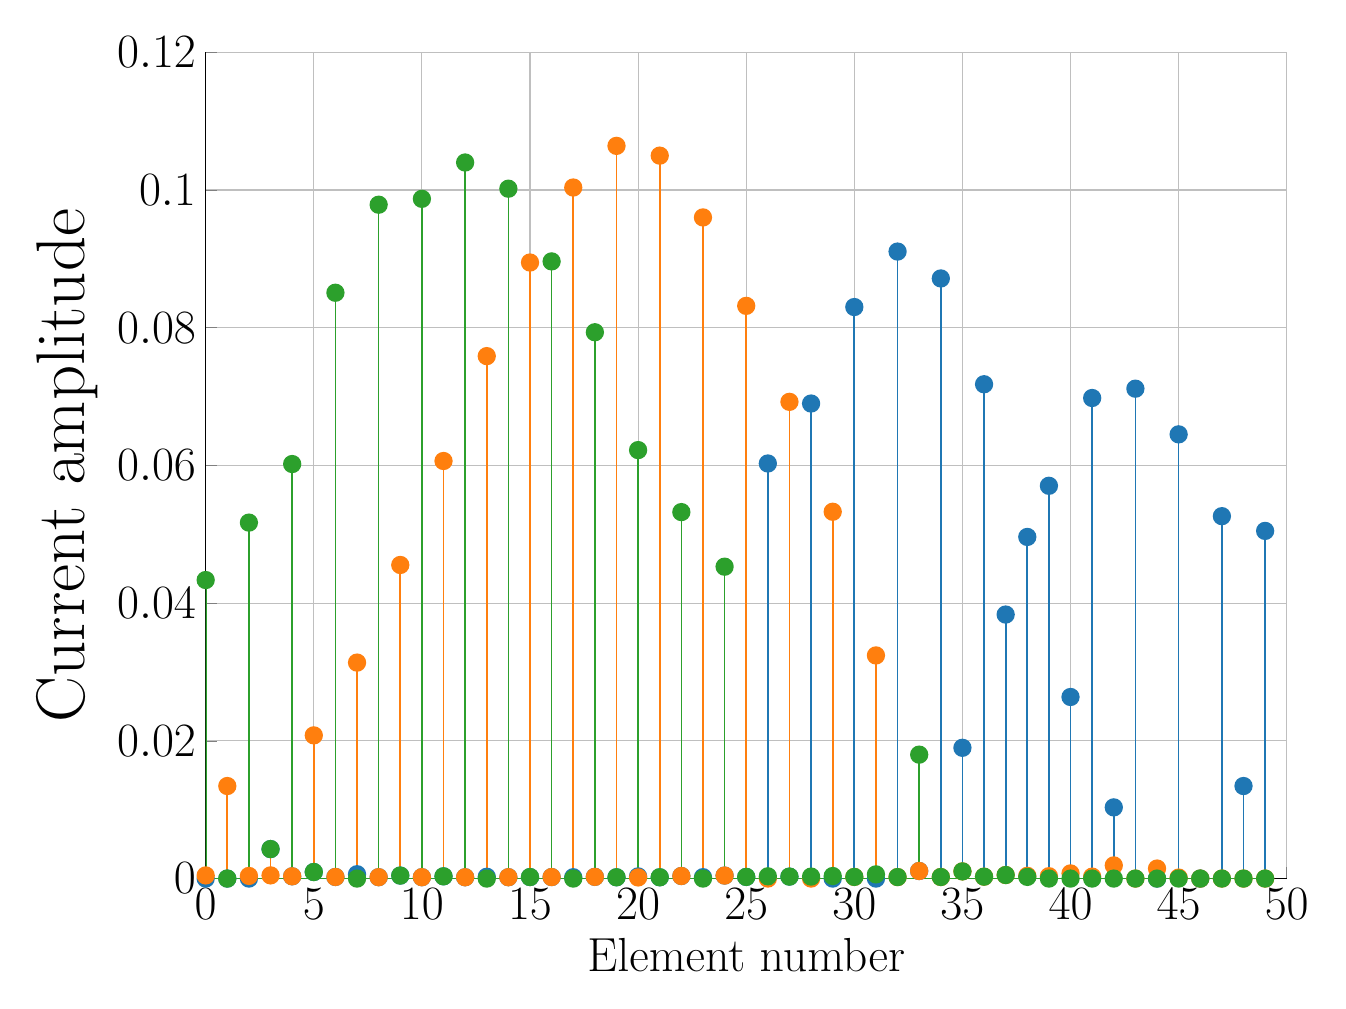
\begin{tikzpicture}

\definecolor{color0}{rgb}{0.12156862745098,0.466666666666667,0.705882352941177}
\definecolor{color1}{rgb}{1,0.498039215686275,0.0549019607843137}
\definecolor{color2}{rgb}{0.172549019607843,0.627450980392157,0.172549019607843}

\begin{axis}[
width=6.028in,
height=4.754in,
at={(1.011in,0.642in)},
% scale only axis,
scaled ticks=false,
tick label style={/pgf/number format/fixed},
xmin=0,
xmax=50,
xlabel={Element number},
xmajorgrids,
ymin=0,
ymax=0.12,
ylabel={Current amplitude},
ymajorgrids,
axis background/.style={fill=white},
axis x line*=bottom,
axis y line*=left,
legend style={legend cell align=left,align=left,draw=white!15!black},
xlabel style={font=\LARGE},ylabel style={font=\Huge},legend style={font=\LARGE},ticklabel style={font=\LARGE}
% legend cell align={left},
% legend style={draw=white!80.0!black},
% tick align=outside,
% tick pos=left,
% x grid style={white!69.01960784313725!black},
% xlabel={Antenna element number},
% xmajorgrids,
% xmin=-2.45, xmax=51.45,
% xtick style={color=black},
% y grid style={white!69.01960784313725!black},
% ylabel={Current amplitude},
% ymajorgrids,
% ymin=-0.0053205899722924, ymax=0.11173238941814,
% ytick style={color=black}
]
\path [draw=color0, semithick]
(axis cs:0,0)
--(axis cs:0,2.1516777304321e-09);

\path [draw=color0, semithick]
(axis cs:1,0)
--(axis cs:1,7.73395355587193e-09);

\path [draw=color0, semithick]
(axis cs:2,0)
--(axis cs:2,6.5347108309423e-08);

\path [draw=color0, semithick]
(axis cs:3,0)
--(axis cs:3,4.28451624448672e-08);

\path [draw=color0, semithick]
(axis cs:4,0)
--(axis cs:4,0.000328566250808884);

\path [draw=color0, semithick]
(axis cs:5,0)
--(axis cs:5,0.00095106665827998);

\path [draw=color0, semithick]
(axis cs:6,0)
--(axis cs:6,0.00023249776901206);

\path [draw=color0, semithick]
(axis cs:7,0)
--(axis cs:7,0.000630656072195389);

\path [draw=color0, semithick]
(axis cs:8,0)
--(axis cs:8,0.000202128182630169);

\path [draw=color0, semithick]
(axis cs:9,0)
--(axis cs:9,0.000434323523352451);

\path [draw=color0, semithick]
(axis cs:10,0)
--(axis cs:10,0.000200381032707694);

\path [draw=color0, semithick]
(axis cs:11,0)
--(axis cs:11,0.000326180621101242);

\path [draw=color0, semithick]
(axis cs:12,0)
--(axis cs:12,0.000190212050891133);

\path [draw=color0, semithick]
(axis cs:13,0)
--(axis cs:13,0.000260701774087729);

\path [draw=color0, semithick]
(axis cs:14,0)
--(axis cs:14,0.000197437994836105);

\path [draw=color0, semithick]
(axis cs:15,0)
--(axis cs:15,0.000221088613655008);

\path [draw=color0, semithick]
(axis cs:16,0)
--(axis cs:16,0.000220689380755874);

\path [draw=color0, semithick]
(axis cs:17,0)
--(axis cs:17,0.000197096664033468);

\path [draw=color0, semithick]
(axis cs:18,0)
--(axis cs:18,0.000249309945527335);

\path [draw=color0, semithick]
(axis cs:19,0)
--(axis cs:19,0.000185890816297607);

\path [draw=color0, semithick]
(axis cs:20,0)
--(axis cs:20,0.000317876974456604);

\path [draw=color0, semithick]
(axis cs:21,0)
--(axis cs:21,0.00018840617423527);

\path [draw=color0, semithick]
(axis cs:22,0)
--(axis cs:22,0.000371663026394869);

\path [draw=color0, semithick]
(axis cs:23,0)
--(axis cs:23,0.000206009960199158);

\path [draw=color0, semithick]
(axis cs:24,0)
--(axis cs:24,0.000436725514819293);

\path [draw=color0, semithick]
(axis cs:25,0)
--(axis cs:25,0.000237822131122286);

\path [draw=color0, semithick]
(axis cs:26,0)
--(axis cs:26,0.0602833563079657);

\path [draw=color0, semithick]
(axis cs:27,0)
--(axis cs:27,0.000285704045130277);

\path [draw=color0, semithick]
(axis cs:28,0)
--(axis cs:28,0.0689897916418297);

\path [draw=color0, semithick]
(axis cs:29,0)
--(axis cs:29,1.58749493750173e-08);

\path [draw=color0, semithick]
(axis cs:30,0)
--(axis cs:30,0.0830039685278625);

\path [draw=color0, semithick]
(axis cs:31,0)
--(axis cs:31,9.43022450452255e-09);

\path [draw=color0, semithick]
(axis cs:32,0)
--(axis cs:32,0.0910604042825212);

\path [draw=color0, semithick]
(axis cs:33,0)
--(axis cs:33,0.00109909008466753);

\path [draw=color0, semithick]
(axis cs:34,0)
--(axis cs:34,0.0871552659029844);

\path [draw=color0, semithick]
(axis cs:35,0)
--(axis cs:35,0.0189911552212102);

\path [draw=color0, semithick]
(axis cs:36,0)
--(axis cs:36,0.0717901459916552);

\path [draw=color0, semithick]
(axis cs:37,0)
--(axis cs:37,0.0383438824438696);

\path [draw=color0, semithick]
(axis cs:38,0)
--(axis cs:38,0.0496146698706208);

\path [draw=color0, semithick]
(axis cs:39,0)
--(axis cs:39,0.0570415498377675);

\path [draw=color0, semithick]
(axis cs:40,0)
--(axis cs:40,0.0263716586926075);

\path [draw=color0, semithick]
(axis cs:41,0)
--(axis cs:41,0.0697920934675394);

\path [draw=color0, semithick]
(axis cs:42,0)
--(axis cs:42,0.0103414981863765);

\path [draw=color0, semithick]
(axis cs:43,0)
--(axis cs:43,0.071145225572326);

\path [draw=color0, semithick]
(axis cs:44,0)
--(axis cs:44,4.36950195272116e-08);

\path [draw=color0, semithick]
(axis cs:45,0)
--(axis cs:45,0.0645132635108412);

\path [draw=color0, semithick]
(axis cs:46,0)
--(axis cs:46,3.44104495509742e-08);

\path [draw=color0, semithick]
(axis cs:47,0)
--(axis cs:47,0.0526318732520428);

\path [draw=color0, semithick]
(axis cs:48,0)
--(axis cs:48,0.0134418006919874);

\path [draw=color0, semithick]
(axis cs:49,0)
--(axis cs:49,0.0504911657418311);

\path [draw=color1, semithick]
(axis cs:0,0)
--(axis cs:0,0.000456230148666515);

\path [draw=color1, semithick]
(axis cs:1,0)
--(axis cs:1,0.0134420736499162);

\path [draw=color1, semithick]
(axis cs:2,0)
--(axis cs:2,0.000382626926252639);

\path [draw=color1, semithick]
(axis cs:3,0)
--(axis cs:3,0.00461685421550746);

\path [draw=color1, semithick]
(axis cs:4,0)
--(axis cs:4,0.000328549904690896);

\path [draw=color1, semithick]
(axis cs:5,0)
--(axis cs:5,0.0207987560646961);

\path [draw=color1, semithick]
(axis cs:6,0)
--(axis cs:6,0.000232479860853123);

\path [draw=color1, semithick]
(axis cs:7,0)
--(axis cs:7,0.0313657575723098);

\path [draw=color1, semithick]
(axis cs:8,0)
--(axis cs:8,0.00020208422270137);

\path [draw=color1, semithick]
(axis cs:9,0)
--(axis cs:9,0.0455443948182072);

\path [draw=color1, semithick]
(axis cs:10,0)
--(axis cs:10,0.000200285236339547);

\path [draw=color1, semithick]
(axis cs:11,0)
--(axis cs:11,0.0606443054179951);

\path [draw=color1, semithick]
(axis cs:12,0)
--(axis cs:12,0.000190088295442947);

\path [draw=color1, semithick]
(axis cs:13,0)
--(axis cs:13,0.0758759348527309);

\path [draw=color1, semithick]
(axis cs:14,0)
--(axis cs:14,0.000197318177478248);

\path [draw=color1, semithick]
(axis cs:15,0)
--(axis cs:15,0.0894708401177406);

\path [draw=color1, semithick]
(axis cs:16,0)
--(axis cs:16,0.000220576218630315);

\path [draw=color1, semithick]
(axis cs:17,0)
--(axis cs:17,0.100361813178148);

\path [draw=color1, semithick]
(axis cs:18,0)
--(axis cs:18,0.000246229474212776);

\path [draw=color1, semithick]
(axis cs:19,0)
--(axis cs:19,0.106411799445848);

\path [draw=color1, semithick]
(axis cs:20,0)
--(axis cs:20,0.000162193315001493);

\path [draw=color1, semithick]
(axis cs:21,0)
--(axis cs:21,0.104991118260313);

\path [draw=color1, semithick]
(axis cs:22,0)
--(axis cs:22,0.000371503595015085);

\path [draw=color1, semithick]
(axis cs:23,0)
--(axis cs:23,0.0960194988797153);

\path [draw=color1, semithick]
(axis cs:24,0)
--(axis cs:24,0.000436623637992223);

\path [draw=color1, semithick]
(axis cs:25,0)
--(axis cs:25,0.0831754013689205);

\path [draw=color1, semithick]
(axis cs:26,0)
--(axis cs:26,2.22920680991619e-06);

\path [draw=color1, semithick]
(axis cs:27,0)
--(axis cs:27,0.0692353261206824);

\path [draw=color1, semithick]
(axis cs:28,0)
--(axis cs:28,2.09879952072849e-07);

\path [draw=color1, semithick]
(axis cs:29,0)
--(axis cs:29,0.0532733872513701);

\path [draw=color1, semithick]
(axis cs:30,0)
--(axis cs:30,0.00023827723464384);

\path [draw=color1, semithick]
(axis cs:31,0)
--(axis cs:31,0.0324074047805182);

\path [draw=color1, semithick]
(axis cs:32,0)
--(axis cs:32,0.000217212424755765);

\path [draw=color1, semithick]
(axis cs:33,0)
--(axis cs:33,0.00109909618173372);

\path [draw=color1, semithick]
(axis cs:34,0)
--(axis cs:34,0.000226951321301935);

\path [draw=color1, semithick]
(axis cs:35,0)
--(axis cs:35,0.00104157154094656);

\path [draw=color1, semithick]
(axis cs:36,0)
--(axis cs:36,0.000275527097623824);

\path [draw=color1, semithick]
(axis cs:37,0)
--(axis cs:37,0.000515864677265231);

\path [draw=color1, semithick]
(axis cs:38,0)
--(axis cs:38,0.000398650870263074);

\path [draw=color1, semithick]
(axis cs:39,0)
--(axis cs:39,0.000346756407919037);

\path [draw=color1, semithick]
(axis cs:40,0)
--(axis cs:40,0.000750011869023874);

\path [draw=color1, semithick]
(axis cs:41,0)
--(axis cs:41,0.000283280755353342);

\path [draw=color1, semithick]
(axis cs:42,0)
--(axis cs:42,0.00191273240032911);

\path [draw=color1, semithick]
(axis cs:43,0)
--(axis cs:43,8.93221610817008e-07);

\path [draw=color1, semithick]
(axis cs:44,0)
--(axis cs:44,0.00145655813851499);

\path [draw=color1, semithick]
(axis cs:45,0)
--(axis cs:45,0.000147405643989791);

\path [draw=color1, semithick]
(axis cs:46,0)
--(axis cs:46,9.72977668732673e-08);

\path [draw=color1, semithick]
(axis cs:47,0)
--(axis cs:47,8.88650146643689e-08);

\path [draw=color1, semithick]
(axis cs:48,0)
--(axis cs:48,4.7325099104895e-08);

\path [draw=color1, semithick]
(axis cs:49,0)
--(axis cs:49,2.96544620566087e-08);

\path [draw=color2, semithick]
(axis cs:0,0)
--(axis cs:0,0.0433564873953393);

\path [draw=color2, semithick]
(axis cs:1,0)
--(axis cs:1,2.88627096700644e-08);

\path [draw=color2, semithick]
(axis cs:2,0)
--(axis cs:2,0.051695969864089);

\path [draw=color2, semithick]
(axis cs:3,0)
--(axis cs:3,4.28411730921915e-08);

\path [draw=color2, semithick]
(axis cs:4,0)
--(axis cs:4,0.0602037783735267);

\path [draw=color2, semithick]
(axis cs:5,0)
--(axis cs:5,0.000951047648830789);

\path [draw=color2, semithick]
(axis cs:6,0)
--(axis cs:6,0.0850802019635869);

\path [draw=color2, semithick]
(axis cs:7,0)
--(axis cs:7,1.09356068017001e-07);

\path [draw=color2, semithick]
(axis cs:8,0)
--(axis cs:8,0.0978634812274079);

\path [draw=color2, semithick]
(axis cs:9,0)
--(axis cs:9,0.000434256533123004);

\path [draw=color2, semithick]
(axis cs:10,0)
--(axis cs:10,0.0987168257972491);

\path [draw=color2, semithick]
(axis cs:11,0)
--(axis cs:11,0.000326083379159946);

\path [draw=color2, semithick]
(axis cs:12,0)
--(axis cs:12,0.103994361446256);

\path [draw=color2, semithick]
(axis cs:13,0)
--(axis cs:13,1.09994912916089e-07);

\path [draw=color2, semithick]
(axis cs:14,0)
--(axis cs:14,0.100188325711606);

\path [draw=color2, semithick]
(axis cs:15,0)
--(axis cs:15,0.000221061369230548);

\path [draw=color2, semithick]
(axis cs:16,0)
--(axis cs:16,0.0896326942324167);

\path [draw=color2, semithick]
(axis cs:17,0)
--(axis cs:17,9.04675613279235e-08);

\path [draw=color2, semithick]
(axis cs:18,0)
--(axis cs:18,0.0793429445661134);

\path [draw=color2, semithick]
(axis cs:19,0)
--(axis cs:19,0.000185837295677191);

\path [draw=color2, semithick]
(axis cs:20,0)
--(axis cs:20,0.0622284559936642);

\path [draw=color2, semithick]
(axis cs:21,0)
--(axis cs:21,0.000188376236898979);

\path [draw=color2, semithick]
(axis cs:22,0)
--(axis cs:22,0.0532229434038526);

\path [draw=color2, semithick]
(axis cs:23,0)
--(axis cs:23,2.53851556308715e-08);

\path [draw=color2, semithick]
(axis cs:24,0)
--(axis cs:24,0.045293903906467);

\path [draw=color2, semithick]
(axis cs:25,0)
--(axis cs:25,0.000237820745609798);

\path [draw=color2, semithick]
(axis cs:26,0)
--(axis cs:26,0.00032813287943533);

\path [draw=color2, semithick]
(axis cs:27,0)
--(axis cs:27,0.000285705981394942);

\path [draw=color2, semithick]
(axis cs:28,0)
--(axis cs:28,0.0002867225731734);

\path [draw=color2, semithick]
(axis cs:29,0)
--(axis cs:29,0.000371310087068562);

\path [draw=color2, semithick]
(axis cs:30,0)
--(axis cs:30,0.00023831269292519);

\path [draw=color2, semithick]
(axis cs:31,0)
--(axis cs:31,0.00061038405704563);

\path [draw=color2, semithick]
(axis cs:32,0)
--(axis cs:32,0.000217225384007144);

\path [draw=color2, semithick]
(axis cs:33,0)
--(axis cs:33,0.0179974197171948);

\path [draw=color2, semithick]
(axis cs:34,0)
--(axis cs:34,0.000226947476303721);

\path [draw=color2, semithick]
(axis cs:35,0)
--(axis cs:35,0.00104158655813998);

\path [draw=color2, semithick]
(axis cs:36,0)
--(axis cs:36,0.000275534181134634);

\path [draw=color2, semithick]
(axis cs:37,0)
--(axis cs:37,0.000515879275661485);

\path [draw=color2, semithick]
(axis cs:38,0)
--(axis cs:38,0.000242653476657279);

\path [draw=color2, semithick]
(axis cs:39,0)
--(axis cs:39,3.75479643391802e-08);

\path [draw=color2, semithick]
(axis cs:40,0)
--(axis cs:40,1.06019977813398e-08);

\path [draw=color2, semithick]
(axis cs:41,0)
--(axis cs:41,6.69892225558733e-09);

\path [draw=color2, semithick]
(axis cs:42,0)
--(axis cs:42,5.61936321645612e-09);

\path [draw=color2, semithick]
(axis cs:43,0)
--(axis cs:43,4.41997510654583e-09);

\path [draw=color2, semithick]
(axis cs:44,0)
--(axis cs:44,3.52265293965403e-09);

\path [draw=color2, semithick]
(axis cs:45,0)
--(axis cs:45,3.1723653343977e-09);

\path [draw=color2, semithick]
(axis cs:46,0)
--(axis cs:46,2.91024265137976e-09);

\path [draw=color2, semithick]
(axis cs:47,0)
--(axis cs:47,2.80479290259624e-09);

\path [draw=color2, semithick]
(axis cs:48,0)
--(axis cs:48,2.94280176858498e-09);

\path [draw=color2, semithick]
(axis cs:49,0)
--(axis cs:49,3.09779795269005e-09);

\addplot [semithick, color0, mark=*, mark size=3, mark options={solid}, only marks, forget plot]
table {%
0 2.1516777304321e-09
1 7.73395355587193e-09
2 6.5347108309423e-08
3 0.00428451624448672
4 0.000328566250808884
5 0.00095106665827998
6 0.00023249776901206
7 0.000630656072195389
8 0.000202128182630169
9 0.000434323523352451
10 0.000200381032707694
11 0.000326180621101242
12 0.000190212050891133
13 0.000260701774087729
14 0.000197437994836105
15 0.000221088613655008
16 0.000220689380755874
17 0.000197096664033468
18 0.000249309945527335
19 0.000185890816297607
20 0.000317876974456604
21 0.00018840617423527
22 0.000371663026394869
23 0.000206009960199158
24 0.000436725514819293
25 0.000237822131122286
26 0.0602833563079657
27 0.000285704045130277
28 0.0689897916418297
29 1.58749493750173e-08
30 0.0830039685278625
31 9.43022450452255e-09
32 0.0910604042825212
33 0.00109909008466753
34 0.0871552659029844
35 0.0189911552212102
36 0.0717901459916552
37 0.0383438824438696
38 0.0496146698706208
39 0.0570415498377675
40 0.0263716586926075
41 0.0697920934675394
42 0.0103414981863765
43 0.071145225572326
44 4.36950195272116e-08
45 0.0645132635108412
46 3.44104495509742e-08
47 0.0526318732520428
48 0.0134418006919874
49 0.0504911657418311
};
\addplot [semithick, color0, forget plot]
table {%
0 0
49 0
};
\addplot [semithick, color1, mark=*, mark size=3, mark options={solid}, only marks, forget plot]
table {%
0 0.000456230148666515
1 0.0134420736499162
2 0.000382626926252639
3 0.000461685421550746
4 0.000328549904690896
5 0.0207987560646961
6 0.000232479860853123
7 0.0313657575723098
8 0.00020208422270137
9 0.0455443948182072
10 0.000200285236339547
11 0.0606443054179951
12 0.000190088295442947
13 0.0758759348527309
14 0.000197318177478248
15 0.0894708401177406
16 0.000220576218630315
17 0.100361813178148
18 0.000246229474212776
19 0.106411799445848
20 0.000162193315001493
21 0.104991118260313
22 0.000371503595015085
23 0.0960194988797153
24 0.000436623637992223
25 0.0831754013689205
26 2.22920680991619e-06
27 0.0692353261206824
28 2.09879952072849e-07
29 0.0532733872513701
30 0.00023827723464384
31 0.0324074047805182
32 0.000217212424755765
33 0.00109909618173372
34 0.000226951321301935
35 0.00104157154094656
36 0.000275527097623824
37 0.000515864677265231
38 0.000398650870263074
39 0.000346756407919037
40 0.000750011869023874
41 0.000283280755353342
42 0.00191273240032911
43 8.93221610817008e-07
44 0.00145655813851499
45 0.000147405643989791
46 9.72977668732673e-08
47 8.88650146643689e-08
48 4.7325099104895e-08
49 2.96544620566087e-08
};
\addplot [semithick, color1, forget plot]
table {%
0 0
49 0
};
\addplot [semithick, color2, mark=*, mark size=3, mark options={solid}, only marks, forget plot]
table {%
0 0.0433564873953393
1 2.88627096700644e-08
2 0.051695969864089
3 0.00428411730921915
4 0.0602037783735267
5 0.000951047648830789
6 0.0850802019635869
7 1.09356068017001e-07
8 0.0978634812274079
9 0.000434256533123004
10 0.0987168257972491
11 0.000326083379159946
12 0.103994361446256
13 1.09994912916089e-07
14 0.100188325711606
15 0.000221061369230548
16 0.0896326942324167
17 9.04675613279235e-08
18 0.0793429445661134
19 0.000185837295677191
20 0.0622284559936642
21 0.000188376236898979
22 0.0532229434038526
23 2.53851556308715e-08
24 0.045293903906467
25 0.000237820745609798
26 0.00032813287943533
27 0.000285705981394942
28 0.0002867225731734
29 0.000371310087068562
30 0.00023831269292519
31 0.00061038405704563
32 0.000217225384007144
33 0.0179974197171948
34 0.000226947476303721
35 0.00104158655813998
36 0.000275534181134634
37 0.000515879275661485
38 0.000242653476657279
39 3.75479643391802e-08
40 1.06019977813398e-08
41 6.69892225558733e-09
42 5.61936321645612e-09
43 4.41997510654583e-09
44 3.52265293965403e-09
45 3.1723653343977e-09
46 2.91024265137976e-09
47 2.80479290259624e-09
48 2.94280176858498e-09
49 3.09779795269005e-09
};
\addplot [semithick, color2, forget plot]
table {%
0 0
49 0
};
\end{axis}

\end{tikzpicture}
            \end{adjustbox}
        \end{column}
\end{columns}   

\end{frame}


%
% -----------------------------------------------------------------------------------------------------------------
%



\end{document}

